\documentclass{report}
\usepackage{suthesis-2e}
\usepackage{hyperref}
\usepackage[capitalise]{cleveref}
\tablespagefalse%


\dept{Computer Science}

%!TEX root = paper.tex
\usepackage[T1]{fontenc} % for tt curly braces
\usepackage{etoolbox} % for various programming stuff
\usepackage{amsmath}
\usepackage{listings}
\usepackage{array}
\usepackage{relsize}
\usepackage{amsthm}
\usepackage{amssymb}
\usepackage{color}
\usepackage[dvipsnames]{xcolor}
\usepackage{graphicx}
\usepackage{booktabs}
\usepackage{fancyvrb}
\usepackage{float}
\usepackage{stringstrings}
\usepackage{stmaryrd}
\usepackage{verbatimbox}
\usepackage{alltt}
\usepackage{multicol}
\usepackage{fixltx2e}
\usepackage[nooneline,bf]{subfigure}
% \usepackage[labelformat=simple]{subcaption}
% \renewcommand\thesubfigure{(\alph{subfigure})}
\usepackage{mdframed}
\usepackage{xcolor}
\usepackage{url}
\usepackage{xspace}
%\renewcommand*{\ttdefault}{txtt}

\lstset{basicstyle=\ttfamily,breaklines=true,columns=fullflexible,keepspaces=true}
% \lstset{columns=flexible}
% \lstset{keepspaces=true}

\newmdenv[
    hidealllines=true,
    backgroundcolor=black!20,
    skipbelow=\baselineskip,
    skipabove=\baselineskip
]{greybox}

\newcommand{\ie}{\emph{i.e.},\xspace}
\newcommand{\eg}{\emph{e.g.},~}
\newcommand{\etal}{\emph{et al.}}

\theoremstyle{definition}
\newtheorem{axiom}{Axiom}
\newtheorem{theorem}{Theorem}
\newtheorem{definition}{Definition}
\newtheorem{lemma}{Lemma}

\newcommand{\I}[1]{\ensuremath{\mathit{#1}}}
\newcommand{\cL}{{\calL}}
\newcommand{\Red}[1]{{\color{red} #1}}
\newcommand{\Blue}[1]{{\color{blue} #1}}
\newcommand{\Updated}[1]{\colorbox{red}{Updated! #1}}

% \newcommand{\Backpack}{\texttt{i}Backpack}%
\newcommand{\OldBackpack}{Backpack'14}%
\newcommand{\Backpack}{Backpack'17}%
\newcommand{\Ccomp}{Resolved component}%
\newcommand{\ccomp}{resolved component}%
\newcommand{\Unit}{Mixed component}%
\newcommand{\unit}{mixed component}%
\newcommand{\Iunit}{Instantiated component}%
\newcommand{\iunit}{instantiated component}%
\newcommand{\cid}{component identifier}%
\newcommand{\Cid}{Component identifier}%
\newcommand{\uid}{unit identifier}%
\newcommand{\Uid}{Unit identifier}%
\newcommand{\ir}{linked intermediate representation}
\newcommand{\Ir}{Linked intermediate representation}

% macros for unit syntax and semantic objects
% ------------------------------
% metavars
\newcommand{\Up}{p}
\newcommand{\UP}{P}
\newcommand{\Un}{n}
\newcommand{\UN}{N}
\newcommand{\UNs}{\mathit{Ns}}
\newcommand{\USn}{\mathit{Sn}}
\newcommand{\Ureqs}{\mathit{mreqs}}
\newcommand{\Uunit}{\mathit{mcomp}}
\newcommand{\mprog}{\mathit{mprog}}
\newcommand{\mcomp}{\mathit{mcomp}}
%\newcommand{\Uudecls}{\mathit{ldecls}}
\newcommand{\Uudecl}{\mathit{mdecl}}
\newcommand{\mdecl}{\mathit{mdecl}}
\newcommand{\mdecls}{\mathit{mdecls}}
\newcommand{\marg}{\mathit{marg}}
\newcommand{\Uhsexps}{\mathit{hsexps}}
\newcommand{\Uhsbody}{\mathit{hsbody}}
\newcommand{\Uhssig}{\mathit{hssig}}
\newcommand{\Uunitty}{\Xi}
\newcommand{\Umty}{T}
\newcommand{\Urole}{R}
\newcommand{\Uty}{\mathit{decl}}
\newcommand{\Utys}{\mathit{decls}}
\newcommand{\Udfun}{\texttt{\$} \I{fn}}
\newcommand{\Uinst}{\mathit{inst}}
\newcommand{\Uinsts}{\mathit{insts}}
\newcommand{\Uimp}{\mathit{orph}}
\newcommand{\Uimps}{\mathit{orphs}}
\newcommand{\Ufinst}{\mathit{finst}}
\newcommand{\Ufinsts}{\mathit{finsts}}
\newcommand{\Umatch}{\mathit{sub}}
% syntax
\newcommand{\UsynUnitH}[2]{\ensuremath{\texttt{component}~#1~#2}}
\newcommand{\UsynUnit}[3]{\ensuremath{\UsynUnitH{#1}{#2}~\{#3\}}}
\newcommand{\UsynMod}[2]{\ensuremath{\texttt{module}~\modnameif{#1}~\{~#2~\}}}
\newcommand{\UsynSig}[2]{\ensuremath{\texttt{signature}~\modnameif{#1}~\{~#2~\}}}
\newcommand{\UsynSigWith}[3]{\ensuremath{\texttt{signature}~\modnameif{#1}~\{~#2~\}~\textsf{with}~#3}}
\newcommand{\UsynDep}[2]{\ensuremath{\texttt{dependency}~#1~(#2)}}
\newcommand{\UsynDepEmpty}[1]{\ensuremath{\texttt{dependency}~#1}}
% semantic objects
\newcommand{\UobjIface}{\texttt{iface}}
\newcommand{\UobjTau}[2]{\ensuremath{\UobjIface\:(#1)~\{#2\}}}
\newcommand{\UobjUnitTy}[4]{\ensuremath{\forall~#1.\, \forall~#2 .\, #3 \rightarrow #4}}
\newcommand{\UobjUnitTyN}[3]{\ensuremath{\forall~#1 .\, #2 \rightarrow #3}}
% ------------------------------



\newcommand{\doubleplus}{\ensuremath{\mathbin{+\mkern-8mu+}}}
\newcommand{\scomp}[2]{\ensuremath{#2 \circ #1}}

\newcommand{\modname}[1]{\ensuremath{\texttt{#1}}}%
\newcommand{\modnameif}[1]{%
  % make the argument a modname if it is not a macro (invocation)
  % and if it is capitalized
  \ifdefmacro{#1}%
    {#1}%
    {%
      \testcapitalized{#1}
      \ifcapitalized 
        \modname{#1}
      \else
        #1
      \fi%
    }%
  % % make the argument a modname if it is not a (primed) "m" or "n" metavar
  % \ifboolexpr{ test {\ifstrequal{#1}{m}} or %
  %              test {\ifstrequal{#1}{m'}} or %
  %              test {\ifstrequal{#1}{m''}} or %
  %              test {\ifstrequal{#1}{n}} or %
  %              test {\ifstrequal{#1}{n'}} or %
  %              test {\ifstrequal{#1}{n''}} }%
  %   {#1}
  %   {\modname{#1}}
}


\newcommand{\hole}[1]{\ensuremath{#1}}%
% \newcommand{\holevar}[1]{\ensuremath{\colorbox{Apricot}{\ensuremath{#1}}}}%
% \newcommand{\holevar}[1]{\ensuremath{\colorbox{Apricot}{\ensuremath{\modnameif{#1}}}}}
\newcommand{\holevar}[1]{\ensuremath{\langle\modnameif{#1}\rangle}}
\newcommand{\nholevar}[1]{\ensuremath{\{\modnameif{#1}\}}}
\newcommand{\hv}[1]{\holevar{#1}}
\newcommand{\nhv}[1]{\nholevar{#1}}

\newcommand{\cidl}[1]{\ensuremath{\mbox{\texttt{#1}}}}%
\newcommand{\cidlif}[1]{
  % make the argument a component ID if it is not a (primed) "p" or "q" metavar
  % NOTE: sometimes "p" is used as a literal! in such cases, use \cidl instead
  \ifdefmacro{#1}%
    {#1}%
    {%
      \ifboolexpr{ test {\ifstrequal{#1}{p}} or %
                   test {\ifstrequal{#1}{p'}} or %
                   test {\ifstrequal{#1}{p''}} or %
                   test {\ifstrequal{#1}{q}} or %
                   test {\ifstrequal{#1}{q'}} or %
                   test {\ifstrequal{#1}{q''}} }%
        {#1}
        {\cidl{#1}}%
    }
}
\newcommand{\icid}[2]{\cidlif{#1}[#2]}
\newcommand{\uidl}[2]{%
  \ensuremath{
    \cidl{#1}%
    [%
      % if subst is non-empty, allow line break after open paren
      \ifstrempty{#2}{}{\allowbreak}%
      #2
    ]%
  }}

% \newcommand{\Mod}[2]{\ensuremath{#1\!:\!#2}}%
\newcommand{\modcolon}{\hspace{.1ex}{:}\hspace{.15ex}}
\newcommand{\Mod}[2]{\ensuremath{#1\modcolon\modnameif{#2}}}%
\newcommand{\MOD}[3]{\ensuremath{\icid{\cidl{#1}}{#2}\modcolon\modnameif{#3}}}%
\newcommand{\subst}[2]{\ensuremath{\modnameif{#1} \mathop{=}\allowbreak #2}}
\newcommand{\substMod}[3]{\subst{#1}{\Mod{#2}{#3}}}
\newcommand{\substMOD}[4]{\subst{#1}{\MOD{#2}{#3}{#4}}}
\newcommand{\substHole}[1]{\subst{#1}{\holevar{#1}}}
\newcommand{\substw}[2]{#1\llbracket#2\rrbracket}
\newcommand{\substww}[3]{#1\llbracket#2\rrbracket\llbracket#3\rrbracket}
\newcommand{\prov}[2]{\ensuremath{\modnameif{#1} \,\mapsto\,\allowbreak #2}}
\newcommand{\provMod}[3]{\prov{#1}{\Mod{#2}{#3}}}
\newcommand{\provMOD}[4]{\prov{#1}{\MOD{#2}{#3}{#4}}}
\newcommand{\provHole}[1]{\prov{#1}{\holevar{#1}}}
\newcommand{\rename}[2]{\ensuremath{\modnameif{#1} \mapsto \modnameif{#2}}}


% now render unit IDs like
%   \uidl{mylib-3.0-aaa}{
%     \subst{m}{M},                                         % m and M are metavars
%     \substMod{Database}{\uidl{mysql-1.0-ccc}{}}{MySQL}    % Database, mysql..., MySQL are rendered
%    }


\newcommand{\haspr}{\:\triangleright\:}
\newcommand{\shapeis}{\triangleright}
%\newcommand{\lctx}{\mathcal{L}}
\newcommand{\lctx}{{\tilde{\Xi}}}
%\newcommand{\provs}{\mathcal{L}_\textsf{prov}}
%\newcommand{\provs}{{\tilde{\Sigma}}_\textsf{P}}
\newcommand{\provs}{{\tilde{\Sigma}}}
\newcommand{\impctx}{\mathcal{L}}
%\newcommand{\reqs}{{\tilde{\Sigma}}_\textsf{R}}
\newcommand{\reqs}{\Theta}
\newcommand{\pre}[1]{\tilde{#1}}
\newcommand{\preprovs}{\mathbb{P}}
\newcommand{\prereqs}{\mathbb{R}}
\newcommand{\preshape}{\mathbb{L}}
\newcommand{\Reqs}{\mathcal{R}}
\newcommand{\preP}{\preprovs}
\newcommand{\preR}{\prereqs}
\newcommand{\preL}{\preshape}
\newcommand{\shctx}{\tilde{\Gamma}}
%\newcommand{\lctxpair}[2]{\langle #1 \,;\, #2 \rangle}
\newcommand{\lctxpair}[2]{\forall #2.\, #1}
%\newcommand{\lctxpair}[2]{\lctxpairx{#1}{#2}}
\newcommand{\lctxpairx}[2]{\forall #2.\, \{ #1 \}}
%\newcommand{\lctxpairx}[2]{\begin{pmatrix}
%\textsf{requires:}& #2 \\
%\textsf{provides:}& #1 \\
%\end{pmatrix}}
\newcommand{\lctxpairex}[2]{\{#2\} &\rightarrow& \{#1\}}
\newcommand{\lift}[1]{\uparrow\!#1}
\newcommand{\shnull}{}
%\newcommand{\shnull}{\cdot}
%\newcommand{\shape}{\tilde{\Xi}}

% curly braces
% \newcommand{\lcb}{{\tt {\char 123}}}
% \newcommand{\rcb}{{\tt {\char 125}}}
\newcommand{\wrapcb}[1]{\texttt{\textbraceleft} #1 \texttt{\textbraceright}}

% S stands for "source", but these are not the true source declarations.

\newcommand{\Scomp}{\I{rcomp}}
\newcommand{\Sincl}{\I{rincl}}
\newcommand{\Sdecl}{\I{rdecl}}
\newcommand{\Scomponent}[2]{\texttt{component}~ #1 ~ \wrapcb{#2}}
\newcommand{\Sinclude}[2]{\texttt{mixin:}~ #1 ~#2}
\newcommand{\Sincludespec}[3]{\texttt{mixin:}~ #1 ~[\texttt{(}#2\texttt{)}]~[\texttt{requires}~ \texttt{(}#3\texttt{)}]}
\newcommand{\Slparen}{\texttt{(}}
\newcommand{\Srparen}{\texttt{)}}
\newcommand{\Sexposed}[2]{\texttt{exposed-module:}~ \modnameif{#1} ~\{ #2 \}}
\newcommand{\Sother}[2]{\texttt{other-module:}~ \modnameif{#1} ~\{ #2 \}}
\newcommand{\Srequired}[2]{\texttt{signature:}~ \modnameif{#1} ~\{ #2 \}}
\newcommand{\Sreexported}[2]{\texttt{reexported-module:}~ \modnameif{#1} ~\texttt{as}~ \modnameif{#2}}
\newcommand{\Sas}[2]{\modnameif{#1} \;\texttt{as}\; \modnameif{#2}}
\newcommand{\Scom}{\texttt{,}\,}

% macros for helper functions
\newcommand{\Freqs}[2][\Delta]{\ensuremath{\mathsf{reqnames}_{#1}(#2)}}
\newcommand{\Fpreshape}[1]{\ensuremath{\mathsf{preshape}(#1)}}
\newcommand{\FpreshapeI}[2][\Delta]{\ensuremath{\mathsf{preshape}_{#1}(#2)}}
\newcommand{\Fprelink}[1]{\ensuremath{\mathsf{merge}(#1)}}
\newcommand{\FprelinkTwo}[2]{\ensuremath{\mathsf{merge}(#1; #2)}}
\newcommand{\Flink}[1]{\ensuremath{\mathsf{link}(#1)}}
\newcommand{\Fsource}[1]{\ensuremath{\mathsf{source}(#1)}}
\newcommand{\Flet}[1]{\ensuremath{\mathsf{bind}(#1)}}
\newcommand{\Fprerename}[3]{\ensuremath{\mathsf{rnthin}(#1; #2; #3)}}
\newcommand{\Frename}[3]{\ensuremath{\mathsf{rnthin}(#1; #2; #3)}}
\newcommand{\Fprovs}[1]{\ensuremath{\mathsf{provs}(#1)}}
\newcommand{\Fdom}[1]{\ensuremath{\mathsf{dom}(#1)}}
\newcommand{\Fexports}[1]{\ensuremath{\mathsf{exps}(#1)}}
\newcommand{\Ftrim}[2]{\ensuremath{\mathsf{trim}_{#1}(#2)}}
\newcommand{\Ffnv}[1]{\ensuremath{\mathsf{fnv}(#1)}}

% notational convenience
\newcommand{\overlinei}[1]{\overline{#1}^i}
\newcommand{\overlinej}[1]{\overline{#1}^j}
\newcommand{\overlinek}[1]{\overline{#1}^k}
\newcommand{\overlinel}[1]{\overline{#1}^l}



\renewcommand{\topfraction}{.85}
\renewcommand{\bottomfraction}{.7}
\renewcommand{\textfraction}{.1}
\renewcommand{\floatpagefraction}{.9}
\renewcommand{\dbltopfraction}{.9}
\renewcommand{\dblfloatpagefraction}{.9}
\setcounter{topnumber}{9}
\setcounter{bottomnumber}{9}
\setcounter{totalnumber}{20}
\setcounter{dbltopnumber}{9}


\newcommand{\Edward}[1]{\textcolor{Red}{\bf[EZY: #1]}}
\newcommand{\Scott}[1]{\textcolor{Plum}{\bf[SK: #1]}}
\newcommand{\Derek}[1]{\textcolor{Blue}{\bf[DD: #1]}}
\newcommand{\Simon}[1]{\textcolor{RedOrange}{\bf[SPJ: #1]}}
\newcommand{\simon}[1]{\Simon{#1}}

% macros for examples

\newcommand{\uidArraysA}{%
  \uidl{arrays-a}{\holevar{Prelude}}%
}
\newcommand{\uidArraysB}{%
  \uidl{arrays-b}{\holevar{Prelude}}%
}
\newcommand{\uidStructures}{%
  \uidl{structures}{\holevar{Prelude}, \holevar{Array}}%
}
\newcommand{\uidStructuresA}{%
  \uidl{structures}{\holevar{Prelude},
                    \Mod{\uidArraysA}{Array}}%
}
\newcommand{\uidStructuresB}{%
  \uidl{structures}{\holevar{Prelude},
                    \Mod{\uidArraysB}{Array}}%
}

\newcommand{\Tmatch}[3]{#1 <:_{#2} #3}
\newcommand{\Tsubg}[3]{\{#1\} \quad #2 \quad \{ #3 \}}
\newcommand{\Tsub}[5]{\{#1\} \quad \Tmatch{#2}{#3}{#4} \quad \{ #5 \}}


\newcommand{\highlight}[1]{%
  \colorbox{yellow!50}{$\displaystyle#1$}}

\newcommand{\graybox}[1]{%
  \colorbox{gray!30}{$\displaystyle#1$}}

\newcommand{\KP}{\mathsf{P}}
\newcommand{\KM}{\mathsf{M}}

\newcommand{\RP}{\mathbb{P}}
\newcommand{\RM}{\mathbb{M}}
\newcommand{\RN}{\mathbb{N}}

\newcommand{\RT}{T}
\newcommand{\RE}{E}

\newcommand{\row}{\textsf{row}}
\newcommand{\rowty}[1]{\llparenthesis{}\,#1\,\rrparenthesis{}}
\newcommand{\record}[1]{\textsf{record}~#1}


\newcommand{\elab}[1]{\ensuremath{\leadsto{} #1}}


\newcommand{\CK}{\mathcal{K}}
\newcommand{\CT}{\mathcal{T}}

\newcommand{\Ictx}{\Gamma_c}
\newcommand{\IGamma}{\Gamma_c}
\newcommand{\IDelta}{\Delta_c}
\newcommand{\Idash}{\vdash_c}
\newcommand{\Impctx}{\impctx_c}
\newcommand{\iprog}{\I{iprog}}
\newcommand{\invariant}{\prec}

\newcommand{\tDelta}{\tilde{\Delta}}
\newcommand{\Quant}{\Theta}
\newcommand{\induces}{\Rightarrow}
% \newcommand{\declst}[3]{\begin{Bmatrix}#1\\#2\\#3\end{Bmatrix}}
\newcommand{\declst}[3]{\begin{Bmatrix}#2\\#3\end{Bmatrix}}
\newcommand{\Ideclst}[2]{\begin{Bmatrix}#1\\#2\end{Bmatrix}}
%\newcommand{\hsubis}{\rightarrow_S}
%\newcommand{\nhsubis}{\rightarrow_{\USn}}


\newcommand{\JMatch}[6]%
  [\Gamma; \Theta; \theta; \Delta; \Up_0]%
  {\ensuremath{#1 \vdash #2 : \forall #3.\, \forall #4.\, #5 \induces #6}}

\newcommand{\JReqType}[4]%
  % [\Gamma; \Up_0; \Theta; \theta; \Delta]%
  [\Gamma; \Theta; \theta; \Delta; \Up_0]%
  {\ensuremath{#1 \vdash #2 \,@\, #3 : #4}}

\newcommand{\thetaOR}{\hat\theta}
\newcommand{\SigmaOR}{\hat\Sigma}

% Alter some LaTeX defaults for better treatment of figures:
    % See p.105 of "TeX Unbound" for suggested values.
    % See pp. 199-200 of Lamport's "LaTeX" book for details.
    %   General parameters, for ALL pages:
    \renewcommand{\topfraction}{0.9}	% max fraction of floats at top
    \renewcommand{\bottomfraction}{0.8}	% max fraction of floats at bottom
    %   Parameters for TEXT pages (not float pages):
    \setcounter{topnumber}{2}
    \setcounter{bottomnumber}{2}
    \setcounter{totalnumber}{4}     % 2 may work better
    \setcounter{dbltopnumber}{2}    % for 2-column pages
    \renewcommand{\dbltopfraction}{0.9}	% fit big float above 2-col. text
    \renewcommand{\textfraction}{0.07}	% allow minimal text w. figs
    %   Parameters for FLOAT pages (not text pages):
    \renewcommand{\floatpagefraction}{0.7}	% require fuller float pages
	% N.B.: floatpagefraction MUST be less than topfraction !!
    \renewcommand{\dblfloatpagefraction}{0.7}	% require fuller float pages

	% remember to use [htp] or [htpb] for placement
        %
\lstset{language=Haskell,keywords={%  
    package, module, signature, link, unit, where, data, import, instance, hiding, type, dependency%
    }%
}%
\lstdefinelanguage{Cabal}
{
  % list of keywords
  morekeywords={
    name,version,library,exposed-modules,signatures,build-depends,main-is,executable,mixins
  },
  alsoletter=-,
  sensitive=false, % keywords are not case-sensitive
  morecomment=[l]{--}, % l is for line comment
  morestring=[b]" % defines that strings are enclosed in double quotes
}


\newcommand{\DIGatoms}{%
    \begin{array}{rcl}
    m & & \mbox{Module name} \\
    p, q & & \mbox{\Cid} \\
    \end{array}
}

\newcommand{\DIGsource}{%
    \begin{array}{rcl}
    \Uhsbody & & \mbox{Module source} \\
    \Uhssig & & \mbox{Signature source} \\
    \end{array}
}

\newcommand{\DIGresolved}{%
    \begin{array}{rcl}
    \Scomp & ::= & \Scomponent{\Up}{\overline{\Sdecl}} \\[0.3em]
    \Sdecl & ::= & \Sinclude{\Up}{\I{rns}} \\
           & |   & \Sexposed{m}{\Uhsbody} \\
           & |   & \Sother{m}{\Uhsbody} \\
           & |   & \Sreexported{m}{m'} \\
           & |   & \Srequired{m}{\Uhssig} \\
    \I{rns} & ::= & [\Slparen\overline{rn}\Srparen]~[\texttt{requires}~ \Slparen\overline{rn'}\Srparen] \\
    \I{rn} & ::= & \Sas{m}{m'} \\
           & |   & m \\
    \end{array}
}

\newcommand{\DIGuid}{%
    \begin{array}{rcll}
      M   &::=& \Mod{\UP}{m} & \text{Module identifier} \\
          &|&   \holevar{m} & \text{Module hole} \\
      \UP &::=& \icid{\Up}{S} & \text{\Uid} \\
      S   &::=& \overline{\subst{m}{M}} & \text{Module substitution} \\
    \end{array}
}

\newcommand{\DIGshape}{%
    \begin{array}{lcll}
    \lctx & ::= & \lctxpairx{\provs}{\reqs} & \mbox{Component shape} \\
    %r_\textsf{R} & ::= & \overline{m \rightarrow m'} & \mbox{Requirement renaming (total)} \\
    %r_\textsf{P} & ::= & \overline{m \rightarrow m'} & \mbox{Provision renaming (partial)} \\
    \reqs  & ::= & \overline{\hv{m}} & \mbox{Required module variables} \\
    \provs & ::= & \overline{\prov{m}{M}}  & \mbox{Provided modules} \\
    \shctx & ::= & \overline{\Up \shapeis \lctx} & \mbox{Component shape context} \\
    \end{array}
}

\newcommand{\DIGmixed}{%
    \begin{array}{rcl}
      \Uunit &::=& \UsynUnit{\Up}{\reqs}{\overline{\Uudecl}} \\
      \Uudecl &::=& \UsynDep{\UP}{r} \\
              &|&   \UsynMod{m}{\Uhsbody} \\
              &|&   \UsynSig{m}{\Uhssig} \\
              %& &   \qquad \textsf{with}~\overline{P\!:\!m} & \quad\text{(Merges)} \\
              %&|&   \UsynLet{m}{M} & \text{Let binding} \\
      %\mprog &::=& \overline{\Uunit} & \text{Mixed program} \\
      r   &::=& \overline{m \mapsto m'} \\
    \end{array}
}

\newcommand{\DIGinterface}{
\begin{array}{rcll}
  %\Uunitty &::=& \forall \Theta.\, \forall \theta.\, \{\Sigma_R\} \rightarrow \{\Sigma_P\}
  %  & \text{Component type} \\
  %\theta &::=& \overline{\hv{m.n}} & \text{Name variable quantifiers} \\
  %\Sigma &::=& \overline{m : \Umty}
  %  & \text{Provided/required types} \\
  %\Gamma &::=& \overline{\Up : \Uunitty} & \text{Component typing context} \\
  \Gamma &::=& \overline{p : \Xi} & \text{Component environment} \\
  \Delta, \Xi &::=& \overline{m : T^s} & \text{Component type} \\
  &&&\\
  \Umty &::=& \UobjTau{\UNs}{\overline{\Uty}~\overline{\Uinst}~\overline{\Uimp}} & \text{Module type} \\
  s &:=& + ~|~ -  & \text{Polarities} \\
  % \tau_R &::=& \exists \overline{\hv{m.n}}.\, \tau  & \text{Signature type} \\
  \UNs &::=& \overline{\UN} & \text{Export list} \\
  \Uty &::=& & \text{Type declarations} \\
       &  |& \texttt{data}~\graybox{n}~\overline{(a ::_\rho \kappa)} & \qquad\text{Abstract data declaration} \\
       &  |& \texttt{class}~\graybox{n}~\overline{(a ::_\rho \kappa)} & \qquad\text{Abstract type class} \\
       &  |& \texttt{type family}~\graybox{n}~\overline{(a :: \kappa)} :: \kappa~\texttt{where}~\texttt{..} & \qquad\text{Abstract closed type family} \\
       &  |& \texttt{data}~\graybox{n}~\overline{(a ::_\rho \kappa)}~\texttt{where}~\I{dinfo}& \qquad\text{Data declaration} \\
       &  |& \texttt{newtype}~\graybox{n}~\overline{(a ::_\rho \kappa)} = \I{ntinfo}& \qquad\text{Newtype declaration} \\
       &  |& \texttt{type}~\graybox{n}~\overline{(a ::_\rho \kappa)} :: \kappa = \tau & \qquad\text{Type synonym} \\
       &  |& \texttt{class}~\graybox{n}~\overline{(a ::_\rho \kappa)}~\texttt{where}~\I{clinfo} & \qquad\text{Type class} \\
       &  |& \texttt{type family}~\graybox{n}~\overline{(a :: \kappa)} :: \kappa~\texttt{where}~\I{tfinfo} & \qquad\text{Closed type family} \\
       &  |& \texttt{type family}~\graybox{n}~\overline{(a :: \kappa)} :: \kappa & \qquad\text{Open type family} \\
       &  |& \texttt{data family}~\graybox{n}~\overline{(a :: \kappa)} :: \kappa & \qquad\text{Data family} \\
       % Patterns omitted
       % Data families omitted
       &  |& n :: \tau& \qquad\text{Term declaration} \\
  % Notes: Why are the axioms/names kept separately from the instance
  % lists, rather than embedded "implicitly" (e.g., like how coercion
  % for newtype is stored)?  Historically, the DFun was always kept
  % separate from the instance declaration.
  \Uinst &::=& \texttt{instance} :: \tau & \text{Class instance} \\
         &  |& \texttt{family instance} :: \I{fiinfo} & \text{Family instance} \\
  \Uimp  &::=& \texttt{orphan}~M & \text{Transitive orphan imports} \\
  &&&\\
  \Un   && \multicolumn{2}{l}{\text{Occurrence name}} \\
  \UN &::=& M.\Un & \text{Original name} \\
      &|&   \nhv{m.n} & \text{Name hole} \\
  \USn &::=& \overline{\subst{m.n}{N}} & \text{Name substitution} \\
  &&&\\
  a &&& \text{Haskell type variable} \\
  \tau &::=& \cdots N \cdots & \text{Haskell type} \\
  \kappa &::=& \cdots N \cdots & \text{Haskell kind} \\
  \rho &::=& \textsf{P} ~|~ \textsf{R} ~|~ \textsf{N} & \text{Role (phantom, representational, nominal)} \\
  \multicolumn{3}{l}{\I{dinfo}, \I{ntinfo}, \I{clinfo}, \I{tfinfo}, \I{fiinfo}} & \text{Haskell declaration metadata} \\
% R &::=& & \text{Haskell role} \\
%   & | & \mathsf{P} & \qquad\text{Phantom} \\
%   & | & \mathsf{R} & \qquad\text{Representational} \\
%   & | & \mathsf{N} & \qquad\text{Nominal} \\
\end{array}
\]\[
\begin{array}{rcl}
\textsf{exports}(\UobjTau{\UNs}{\Utys\, \Uinsts\, \Uimps} &\defeq& \UNs \\
\textsf{decls}(\UobjTau{\UNs}{\Utys\, \Uinsts\, \Uimps} &\defeq& \Utys \\
\textsf{insts}(\UobjTau{\UNs}{\Utys\, \Uinsts\, \Uimps} &\defeq& \Uinsts \\
\textsf{orphs}(\UobjTau{\UNs}{\Utys\, \Uinsts\, \Uimps} &\defeq& \Uimps \\
\textsf{occname}(\nhv{m.n}) &\defeq& n \\
\textsf{occname}(M.n) &\defeq& n \\
\textsf{occname}(\Uty) &\defeq& \graybox{n} \quad(\text{see production for \I{decl}}) \\
\UNs(n) &\defeq& N ~\textsf{where}~ N \in \UNs \land \textsf{occname}(N) = n \\
\Utys(n) &\defeq& \Uty ~\textsf{where}~ \Uty \in \Utys \land \textsf{occname}(\Uty) = n \\
\textsf{nsubst}(m, \overline{N_i}) &\defeq& \overline{\nhv{m.{\sf occname}(N_i)} \mapsto N_i}
\end{array}
}


\DeclareMathOperator{\dom}{dom}

\newcommand{\ctx}{\Gamma; \Delta; P_0}

\newenvironment{twocol}
  {
    \setlength{\abovedisplayskip}{0pt}
    \setlength{\belowdisplayskip}{0pt}
    \begin{tabular}{ m{0.47\textwidth} m{0.47\textwidth} }
  }
  { \end{tabular} }

\newenvironment{shortmath}
  {
    \setlength{\abovedisplayskip}{4pt}
    \setlength{\belowdisplayskip}{0pt}
  }
  {  }

\newcommand\defeq{\mathrel{\overset{\makebox[0pt]{\mbox{\normalfont\tiny def}}}{=}}}

\newenvironment{grayframe}%
  {\begin{mdframed}[backgroundcolor=black!10,linewidth=0,skipabove=0pt,skipbelow=0pt]}%
  {\end{mdframed}}


\begin{document}
\title{Backpack: Towards Practical Mix-in Linking in Haskell}
\author{Edward Z. Yang}
\principaladviser{David Mazi\`eres}
\firstreader{Derek Dreyer}
\secondreader{John Mitchell}
%\thirdreader{Jane Supernumerary} %if needed
%\fourthreader{Severus Snape} %if needed

\beforepreface%
%\prefacesection{Preface}
%    (To be written)
\prefacesection{Acknowledgments}
    I want to thank David Mazi\`eres for his help, advice, and
    willingness to let me go off and explore the strange world
    of module systems for Haskell.  He always stepped up to the bat
    when I needed it.  I also have to thank my coadvisor John
    Mitchell for his sage advice and his CS242 syllabus---without
    which I would have lost much more sleep teaching at Stanford.

    This thesis would not exist without the work of Scott Kilpatrick.
    Backpack is really two PhDs of work: Scott did the theory, I did the
    implementation.  He really is my academic better half.  I also have
    to thank Derek Dreyer who acted as a remote technical advisor
    while I was in the weeds.
    I would not have come to do a PhD in the first place without the
    superb mentorship of Simon Peyton Jones and Simon Marlow.  They are,
    and continue to be, an inspiration to me.

    Many individuals both inside and outside of Stanford have helped
    make the PhD journey a little less lonely.  At risk of forgetting
    someone, they include Deian Stefan, Ali Mashtizadeh, Sergio Benitez,
    Amit Levy, David Terei, Adam Belay, Daniel Giffin, Alejandro Russo,
    Petr Marchenko, Henry Corrigan-Gibbs, Riad Wahby, Danae Metaxca,
    Stefan Heule, Ryan Newton, Giovanni Campagna, Andreas Rossberg and
    Mary-Jane Swenson.

    I would also like to thank Mom, Dad, and my two brothers, James
    and David, for being a rock of unconditional support and love,
    both before and during my PhD.

    And last but not least, I would like to thank Kaixi Ruan, love
    of my life.  This one's for you.
\afterpreface%

%!TEX root = paper.tex
\chapter{Introduction}
\label{sec:intro}

% Here is a problem
% It's an interesting problem
% It's an unsolved problem
% Here is my idea

% Describe the problem
% State your contributions



%   Here are the parameters of the problem:

%   \begin{itemize}
%       \item We want to support separate modular development in Haskell,
%       for all the reasons we've stated above (ability to abstract over
%       implementation, giving you the ability to swap out components.
%       Extreme implementation changes.)

%       \item What do we want to abstract over? We want to abstract
%       over packages.  This is because packages are the way large
%       scale software is distributed.

%       \item But there is an abstraction barrier between the compiler
%       and the package system.  How to design a system that respects
%       this barrier.  (Why is this hard?)
%   \end{itemize}




% The case for separate modular development
% The case for separate modular development at the package level

% The basic idea


% Large software is made of packages.
% Packages are not modular.
% Idea of separate modular development.
% SMD is not done at package level

The essence of modular development is to decompose a program into
collection of smaller modules separated by abstraction barriers: the
defining characteristic of a modular program is the ability of a module to
operate without knowing the implementation details of another.  Modular
programs are easier to understand; opportunities to reuse modular
components are everywhere:

\begin{itemize}
    \item Suppose you are writing an application which makes a request to
    some external backend service---perhaps a database or a credit card
    processor.  You might want to modularize your
    application so that you can \emph{swap} out the real implementation
    of a service with a fake, so that you can test your application without
    charging your customers.

    \item Suppose you are writing a library that handles strings in some
    way---perhaps a parser or a string processing library.  Usually, your
    library doesn't require a specific representation; in fact, you would
    like your library to be \emph{parametric} over all the string representations
    your clients might use (whether it is linked lists of
    characters, packed bytestrings, packed UTF-16 strings, packed UTF-8
    strings\ldots).

    \item Suppose you have two implementations of an API\@: a simple but
    inefficient reference implementation and a complicated but
    fast production implementation.  You might like to \emph{instantiate}
    an application with both implementations and then run them in
    parallel, comparing their outputs to verify the correctness of the
    production implementation.
\end{itemize}
%
Typically, programming languages provide support for both \emph{incremental
modular development}, where module can be developed only when implementations
of its dependencies are available, and \emph{separate modular development},
where a module can be developed with respect to an \emph{interface}
and instantiated later.  Haskell's existing module system is a mechanism
for incremental modular development---it is purely a namespace management
mechanism with a proper concept of interface---while Haskell's type classes are a
mechanism for separate modular development.  Separate modular development
offers more abstraction, as the interface characterizes
what is needed from a dependency.

Unfortunately, type classes are ill-suited for certain cases of
separate modular development:

\begin{itemize}
    \item From a code perspective, type class parametric code is often
    harder to use than monomorphic code.  For an inexperienced
    Haskeller, the proliferation of constraints and type parameters in the
    type signatures of functions can make an otherwise straightforward
    API impenetrable:\footnote{\url{https://hackage.haskell.org/package/regex-posix-0.95.2/docs/Text-Regex-Posix-Wrap.html}}

\begin{lstlisting}
    (=~) :: (RegexMaker Regex CompOption ExecOption source,
             RegexContext Regex source1 target)
         => source1 -> source -> target -- from regex-posix-0.95.2
\end{lstlisting}

    Furthermore, type classes work best when exactly a single type
    parameter is involved in instance resolution. If there aren't any type
    parameters, you must introduce a proxy type to drive instance resolution; if
    there are multiple parameters~\cite{lfp92}, you often need to resolve ambiguity
    by introducing functional
    dependencies~\cite{Jones:2000:TCF:645394.651909} or replacing
    parameters with associated types~\cite{towards-open-type-functions-haskell}.

    \item Type classes work best when it is clear what methods they
    should support.  However, for many interfaces, it is not obvious
    what set of methods should be put into an interface; for example,
    there are many functions which an interface for strings might
    support---which ones go in the type class?  It is inconvenient
    to define a new type class (and new instances) just to add a
    few more methods, and thus this is rarely done in practice.

    \item From a performance perspective, code which uses a type class
    is compiled without knowledge of how the type class's
    methods are implemented.  This can be quite costly in a language
    like Haskell, where inlining definitions is essential to achieving
    good performance.~\cite{PeytonJones:2002:SGH:968417.968422}  This problem can
    be mitigated by specializing code to a particular type, but if this
    specialization occurs at use-site, the compiler ends up repeatedly reoptimizing
    the same function, blowing up the code size of
    a program. (C++ templates suffer from similar problems.\footnote{\url{https://gcc.gnu.org/onlinedocs/gcc/Template-Instantiation.html}})
\end{itemize}
%
In short, Haskell would be well served by an extension to its module
system to support the cases of separate modular development which are
currently poorly served by type classes.

The Backpack package system by Scott Kilpatrick et al.~\cite{backpack}
(hereafter called \OldBackpack{}) broke new ground, arguing that \emph{mixin
packages} could be a good fit for providing modularity in Haskell.
The two words ``mixin'' and ``package'' capture the key properties of \OldBackpack{}:

\begin{itemize}
    \item \emph{Mixins}. Mixin modules~\cite{bracha+:modularity,ancona+:cms,flatt+:units,duggan:mixin} are characterized by components which both \emph{provide} and \emph{require}
    modules:  these components can be ``mixed'' together, linking
    together provisions and requirements which have
    the same name.  Unlike the more conventional approach of
    \emph{parametrized} modules (ala ML~\cite{milner+:def-of-sml-revised}),
    mixin modules natively support recursive linking.
    Furthermore, mixins help reduce
    the preponderance of \emph{sharing constraints} that occur with ML
    functors, since requirements can be mixed together by name.
    (For more discussion on this, see Appendix~\ref{sec:mixins-reduce-sharing-constraints})

    \item \emph{Packages}. Rather than introduce a new module language
    to the compiler, \OldBackpack{} proposed that mixins be added to
    Haskell's package system.  There are multiple benefits to this choice.
    First, it allows us to retrofit Haskell to support separate modular
    development without requiring ``yet another type system extension.''
    Second, it means that Haskell code can be made more
    modular without having to adopt the ``fully-functorized'' style~\cite{structabshotlang}
    commonly associated with ML functors.
    Finally, it brings modularity to the place where it matters most:
    software development in the large;  after all, \emph{packages} are how
    software systems are organized at the largest scale.
\end{itemize}
%
There was just one problem: despite its emphasis on being a practical
design, \OldBackpack{} could not be implemented in a real world compiler
like GHC\@.  Why not? The
semantics of \OldBackpack{}, especially its package-level semantics,
were closely entwined with the semantics of Haskell itself,  violating
the traditional abstraction barrier between the compiler and package
manager.  Without tightly coupling GHC (the Haskell compiler) and Cabal
(the Haskell package manager), there was no way to directly implement
\OldBackpack{}.

In this thesis, we show how to refactor
\OldBackpack{} to respect the abstraction barrier between the package
manager and the compiler, giving us a new system: \Backpack{}.  In
particular, we divide \Backpack{} into two parts: \emph{mixin linking}
which is indifferent to Haskell source code, and \emph{typechecking against
interfaces}, which is purely the concern of the compiler.

Specifically, the contributions of this thesis are as follows:
\begin{itemize}

    \item We describe a package language which can be \emph{mixin
    linked} without knowing anything about the Haskell programming
    language. (\cref{sec:mix-in})  This gives us a language agnostic mechanism for
    expressing separate modular development, in contrast to
    \OldBackpack{}, whose semantics critically relies on the import structure
    of Haskell modules.  As a result, \Backpack{}
    employs a far simpler mixin linking procedure essentially equivalent
    to early descriptions of mixin linking in the literature.~\cite{cardelli:linksets}
    In doing so, we adjust \OldBackpack{}'s primary technical device,
    the \emph{module identity} into a new concept, the \emph{unit identity} (\cref{sec:uid}),
    which can be computed by language agnostic mixin linking.
    Our new package language is order-independent, which is
    essential for backwards-compatibility with Haskell's existing
    package format.

    \item To express the results of mixin linking, we introduce the
    \emph{\unit{} language}, an intermediate representation that
    represents all instantiations explicitly.  This language is reminiscent of
    ML-style applicative functors, but with a twist:
    unfilled requirements of dependency are propagated to the requirements
    of the enclosing package via the process of \emph{signature merging}.
    The effect is that \Backpack{}, as a whole, has similar
    semantics to the ones that were pioneered by \OldBackpack{}.

    \item We describe how to typecheck the \emph{\unit{} language} in the
    real world (\cref{sec:compiler}), typechecking the source into semantic objects that
    faithfully reflect the full glory of GHC Haskell's type system.
    We give an unsound but pragmatic mechanism for supporting \emph{type classes}
    (it is unsolvable in the presence of open type families), support
    the use of \emph{type synonyms} to implement abstract data
    (not supported by \OldBackpack{}), and describe
    some tricky interactions with GHC's type inference algorithm and
    roles annotations.

    \item This is not a paper design: Backpack has been fully
    implemented GHC 8.2 and cabal-install 2.0.
    We give a tour of the modifications we made to GHC to
    implement the necessary instantiation and merging operations
    required by the \unit{} language, as well as the architectural
    changes that were necessary in Cabal (the package manager)
    to orchestrate the typechecking and building of the mixin
    packages. (\cref{sec:implementation})

    \item Does \Backpack{} work?
    We have done a number of case studies to give evidence
    that \Backpack{} works, including conversions of complex,
    real-world packages to use \Backpack{}. (\cref{sec:evaluation})

%   Among other things, these case studies
%   have motivated the introduction of \emph{signature thinning}
%   and how Backpack interoperates with Cabal's existing dependency
%   solver.

\end{itemize}
%
%   In this thesis, we do not address
%   mutual recursion between packages, allowing us to avoid some orthogonal
%   technical complications. We believe that in practice this is a minor
%   limitation.
Although the idea of separating the core language and the module/package
language is not novel~\cite{leroy:modular,milner+:def-of-sml-revised,rossberg+:f-ing}, we are the first to exploit these ideas in service
of an actual implementation, retrofitting strong modularity to an existing
programming language.  The true test of \Backpack{} will be whether or not
the larger Haskell community adopts it, which can only be seen in the
coming years, but we have enough experience working with \Backpack{}
that we believe that this design is practical and solves many problems
that Haskell programmers face today.




%%% Local Variables:
%%% mode: latex
%%% TeX-master: "paper"
%%% End:

%!TEX root = paper.tex
\chapter{A tutorial of \Backpack{}}
\label{sec:tour}

In this section, we will walk through a tutorial of taking a Haskell'98
regular expression matcher taken
from~\cite{Fischer:2010:PRE:1863543.1863594}, highlighting the main
features of \Backpack{} as well as introducing some core conceptual
ideas which will be elaborated upon later in this thesis.  We'll assume
familiarity with Haskell'98 or an ML-like language but won't assume you
know anything about Cabal (Haskell's package management system) or
\OldBackpack{}~\cite{backpack}.\footnote{For a more copy-paste friendly
version of this tutorial, please refer to \url{http://blog.ezyang.com/2016/10/try-backpack-ghc-backpack/}}

\section{A simple matcher in '98}

In Figure~\ref{fig:matcher-haskell98}, we reproduce the source code of
a simple regular expression matcher
from Fischer, Huch and Wilke~\cite{Fischer:2010:PRE:1863543.1863594},
along with a small test program.  We'll use this code to briefly
describe how Haskell's existing module and package system works;
experienced readers should feel free to skip ahead to the next section.

\begin{figure}
\begin{lstlisting}
module Regex (Reg(..), accept) where

-- | A type of regular expressions.
data Reg = Eps | Sym Char | Alt Reg Reg | Seq Reg Reg | Rep Reg

-- | Check if a regular expression 'Reg' matches a 'String'
accept :: Reg -> String -> Bool
accept Eps       u = null u
accept (Sym c)   u = u == [c]
accept (Alt p q) u = accept p u || accept q u
accept (Seq p q) u = or [accept p u1 && accept q u2 | (u1, u2) <- splits u]
accept (Rep r)   u = or [and [accept r ui | ui <- ps] | ps <- parts u]

-- | Compute all splits of the string.
splits :: String -> [(String, String)]
splits [] = [([], [])]
splits (c:cs) = ([], c:cs):[(c:s1,s2) | (s1,s2) <- splits cs]

-- | Compute all possible non-empty partitions of the string
parts :: String -> [[String]]
parts [] = [[]]
parts [c] = [[[c]]]
parts (c:cs) = concat [[(c:p):ps, [c]:p:ps] | p:ps <- parts cs]
\end{lstlisting}
\caption{Source code for a regular expression matcher from~\cite{Fischer:2010:PRE:1863543.1863594}.}
\begin{lstlisting}
module Main where

import Regex

nocs = Rep (Alt (Sym 'a') (Sym 'b'))
onec = Seq nocs (Sym 'c')
evencs = Seq (Rep (Seq onec onec)) nocs
main = print (accept evencs "acc")
\end{lstlisting}
\caption{Simple test program for the matcher.}
\label{fig:matcher-haskell98}
\end{figure}

Looking at the source code, we can observe a few things:

\begin{itemize}
    \item The code is organized into two \emph{modules}, each heralded
    by the \verb|module| keyword.  Each module defines types and values
    within a distinct namespace.  In fact, Haskell modules are used purely for
    namespacing and do not support any sort of hierarchical organization.

    \item The \verb|import| keyword is used to bring declarations into
    scope from other modules; for example, \verb|Main| imports \verb|Regex|
    to bring the constructors of \verb|Reg| and \verb|accept| into scope.
    Every module also implicitly has an import of \verb|Prelude|, which
    provides many commonly used types and functions (e.g., \verb|print|,
    \verb|String|, etc).

    \item The \verb|Regex| module comes with an \emph{export list}
    \verb|(Reg(..), accept)|, which designates which declarations should
    be brought into scope when this module is imported.  The ability to
    omit declarations from an export list (e.g., \verb|splits| and \verb|parts|)
    is one of the primary mechanism by which data abstraction is achieved in
    Haskell: internal implementation details are not exported and thus
    cannot be accessed by end users.
\end{itemize}
Modules themselves are organized into packages, which are described by
\emph{Cabal files}.  For example, the modules above might be organized into
packages with the Cabal files as shown in Figure~\ref{fig:matcher-packages}.
Each package description describes:

\begin{figure}
\begin{tabular}{p{0.45\textwidth} p{0.45\textwidth}}
\begin{lstlisting}[language=Cabal]
-- regex.cabal
name: regex
version: 1.0
library
    exposed-modules: Regex
    build-depends: base
\end{lstlisting}
&
\begin{lstlisting}[language=Cabal]
-- regex-program.cabal
name: regex-program
version: 1.0
executable regex-program
    main-is: Main.hs
    build-depends: base, regex
\end{lstlisting}
\end{tabular}
\caption{Cabal files for the regex and regex-program packages. The Haskell source code
of these packages is in Figure~\ref{fig:matcher-haskell98}.}
\label{fig:matcher-packages}
\end{figure}

\begin{itemize}
    \item The name of the package (\verb|name|),
    \item The version of a package (\verb|version|),
    \item One or more \emph{components} (libraries, executables,
    test-suites, etc.), each of which defines some modules
    (\verb|exposed-modules| and \verb|main-is|) and specifies
    dependencies on libraries of other packages (\verb|build-depends|).
    A library exposes modules for other packages to use when
    they \verb|build-depends| on the library, while an
    executable is associated with a particular \verb|hs| file
    which is expected to define a \verb|main| function that
    will serve as the top-level entry of the program.\footnote{For the
    sake of realism, each package above includes \texttt{base} in their
    \texttt{build-depends}, to ensure that the implicitly imported
    \texttt{Prelude} module is in scope.}
\end{itemize}
Packages serve as the unit of distribution: a set of modules organized
into a package can be uploaded to a package repository (e.g., Hackage\footnote{\url{https://hackage.haskell.org/}})
to be shared with other developers.  A \emph{package
manager} (e.g., cabal-install) automates the process of downloading the source code of all
packages one needs and building them in dependency order.

\section{Functorizing the matcher}

One problem with the code in Figure~\ref{fig:matcher-haskell98} is that
it only works with \verb|String|s (i.e., \verb|[Char]|).  One easy
generalization (seen in the original
paper~\cite{Fischer:2010:PRE:1863543.1863594}) is to add a type
parameter to \verb|Reg|, so that \verb|accept| operates on lists of
arbitrary symbols rather than just characters.  But this is still not as
general as the matcher could be; for example,
\verb|ByteString| is not a list but a packed array of bytes.
We can only support \verb|ByteString| if we are also parametric in the string type itself.

In this case, we can use \Backpack{} to functorize our matcher over an
arbitrary string and element type.  To do this, we create a new
signature named \verb|Str|, which provides abstract string and element
types, and all the string operations our matcher requires.
The resulting signature and module can be seen in
Figure~\ref{fig:matcher-regex-indef-source}, alongside a module which
implements the string signature.

\begin{figure}
\begin{lstlisting}
signature Str where

data Str
data Chr
instance Eq Str

null      :: Str -> Bool
singleton :: Chr -> Str
splits    :: Str -> [(Str, Str)]
parts     :: Str -> [[Str]]
\end{lstlisting}
\caption{Source code for a signature specifying abstract strings.}

\begin{lstlisting}
module Regex where

import Prelude hiding (null)
import Str

data Reg = Eps | Sym Chr | Alt Reg Reg | Seq Reg Reg | Rep Reg

accept :: Reg -> Str -> Bool
accept Eps       u = null u
accept (Sym c)   u = u == singleton c
accept (Alt p q) u = accept p u || accept q u
accept (Seq p q) u = or [accept p u1 && accept q u2 | (u1, u2) <- splits u]
accept (Rep r)   u = or [and [accept r ui | ui <- ps] | ps <- parts u]
\end{lstlisting}
\caption{Source code for regular expression matcher, parametrized by the Str signature.}
\label{fig:matcher-regex-indef-source}
\end{figure}

Because the original source code of the matcher was not written with
this functorization in mind, the \verb|Regex| module must be modestly
refactored to treat \verb|Str| abstractly.  We replaced the
use of list operations \verb|null| and \verb|[c]| with abstract
functions and deleted the implementations of \verb|splits| and
\verb|parts|, deferring them to the signature implementation.  However,
no invasive changes---e.g., adding new type parameters or passing new
arguments---were necessary.  The new Cabal file for this signature and
module, seen in Figure~\ref{fig:matcher-regex-indef-cabal}, needs only
to declare \verb|Str| in the \verb|signatures| field.
The new \verb|regex-indef| package can be typechecked without an
implementation of \verb|Str|.

\begin{figure}
\begin{lstlisting}[language=Cabal]
name: regex-indef
version: 1.0
library
    exposed-modules: Regex
    signatures: Str
    build-depends: base
\end{lstlisting}
\caption{Cabal files for the regex-indef package, which provides a Regex
module parametrized by string implementation.}
\label{fig:matcher-regex-indef-cabal}
\end{figure}

\section{An implementation of Str}

Before we instantiate \verb|regex-indef|, we will need an implementation
of the \verb|Str| signature.  Figure~\ref{fig:matcher-str-string-source}
provides one such implementation (the implementations of \verb|splits| and
\verb|parts| are copy-pasted from Figure~\ref{fig:matcher-haskell98}).

\begin{figure}
\begin{tabular}{p{0.55\textwidth} p{0.40\textwidth}}
\begin{lstlisting}
module Str.String where

import Prelude as P

type Str = String
type Chr = Char

null   = P.null :: Str -> Bool
singleton = (\c -> [c]) :: Chr -> Str
splits = ... :: Str -> [(Str, Str)]
parts  = ... :: Str -> [[Str]]
\end{lstlisting}
&
\begin{lstlisting}[language=Cabal]
name: str-string
version: 1.0
library
    exposed-modules: Str.String
    build-depends: base
\end{lstlisting}
\end{tabular}
\caption{An implementation of Str, alongside its package description.}
\label{fig:matcher-str-string-source}
\end{figure}

One thing to
note is that we must declare \verb|null| and \verb|singleton| with
explicit type signatures, as signature matching in Haskell requires two
declarations to have exactly the same type: the polymorphic function
\verb|[a] -> Bool| is not considered a valid implementation of
\verb|[Char] -> Bool|. \Red{Discuss what would be involved with
better subtyping.}

%   Signatures in Backpack are width-subtyped, so
%   \verb|Str.String| could also contain more exported functions and still
%   be considered to implement \verb|Str|.

%   In practice, the current convention in the Haskell community when
%   defining new modules is to pick a new name.  Thus, it's more likely
%   that the \verb|Str| module from \verb|str-string| will actually
%   be named something like \verb|Str.String|.  In this case,

\section{Instantiating the matcher}

How do we instantiate our matcher with the
implementation of Str from Figure~\ref{fig:matcher-str-string-source}?
In a traditional, ML module system, there would be a module language for
expressing how to instantiate a functor.
In \Backpack{}, a client instantiates a package by bringing its
requirements into scope with another module under the same name,
as seen in the package description in Figure~\ref{fig:matcher-functorized-packages}.  Here, the executable \verb|regex-program| uses the
\verb|mixins| field to rename the module from \verb|str-string| to the
same name as \verb|regex-indef|'s signature; when a module and
a signature have the same name, they are \emph{mix-in linked} together.%
%
\footnote{Why didn't \texttt{str-string} just export
a module named \texttt{Str}?  The prevailing convention in the Haskell
community is that modules should be given unique names; naming all
implementations of the \texttt{Str} signature \texttt{Str} would violate
this convention.  At this point in time, it's not clear if the
convenience of not needing to rename modules overrides the benefits of
being able to refer to a module uniquely by its name.}

\begin{figure}
\begin{lstlisting}[language=Cabal]
name: regex-program
version: 1.0
executable regex-program
    main-is: Main.hs
    build-depends: base, regex-indef, str-string
    mixins: str-string (Str.String as Str)
\end{lstlisting}
\caption{Package descriptions for \texttt{regex-program}, which brings
Regex into scope instantiated with the \texttt{Str} implementation from \texttt{str-string}.}
\label{fig:matcher-functorized-packages}
\end{figure}

What actually happens when mix-in linking takes place?  There are two very useful
ways to understand the process.  In Figure~\ref{fig:regex-indef-instantiated}, we
\emph{pictorially} represent each depended upon library as a block, with input and output
ports representing signatures and modules respectively.  Intuitively, the process
of mix-in linking involves ``wiring up'' these signatures and modules by matching
up names which are the same.

\begin{figure}
\center%
\includegraphics{figures/regex-indef-instantiated.pdf}
\caption{This is the wiring diagram for regex-program. The left side of blocks
(representing libraries) have input ports (required signatures), while the right hand side
of blocks have output ports (provided modules). Ports are wired to show how requirements are
filled: a kink indicates some renaming took place. Mixin linking wires up requirements
and provisions which have the same module name.}
\label{fig:regex-indef-instantiated}
\end{figure}

We can also consider an intermediate representation of the package language
\emph{after} mix-in linking,
as in Figure~\ref{fig:matcher-bkp}, where every dependency on another library
is given an \emph{explicit instantiation} specifying how all of its requirements
are filled---a \emph{syntactic} interpretation of
the package description. We can identify a library plus an instantiation by
specifying a \emph{\uid{}}.  In the case of \verb|regex-indef|, the
\uid{} indicates that the requirement \verb|Str| is to be filled
with the module \verb|Str.String| from the library \verb|str-string|.\footnote{In
fact, GHC 8.2 comes with a mode for directly parsing and compiling this intermediate
representation, which is used extensively by our test suite.}  This intermediate
representation will play an important role in managing the abstraction barrier
between the compiler and package manager, and we will repeatedly return to
it throughout the rest of this thesis.

\begin{figure}
\begin{lstlisting}
unit regex-program where
    dependency base
    dependency str-string
    dependency regex-indef[Str=str-string:Str.String]
    module Main where ...
\end{lstlisting}
\caption{The intermediate representation of the packages from Figure~\ref{fig:matcher-functorized-packages}.
The reference to \texttt{regex-indef} in \texttt{regex-program} now consists of an explicit functor application.}
\label{fig:matcher-bkp}
\end{figure}

One important practical consideration is whether or not there is any
performance cost to using signatures, deferring the implementation of
a module until later.  In particular, if one separately
compiles uninstantiated components to machine code, no cross-package
inlining can occur, since the component is compiled only against a
signature and not against the code that implements the signature.  For
Haskell and GHC, cross-module inlining is a major contributor to
performance~\cite{PeytonJones:2002:SGH:968417.968422}, so our implementation of \Backpack{} does \emph{not}
separately compile uninstantiated packages. Instead, every distinct
instantiation of a component is compiled against the code that
implements its requirements. This process is managed by Cabal to avoid
unnecessary recompilation, similarly to how Cabal avoids recompiling
dependencies that are already installed.

\section{Reusing libraries with different instantiations}

The reason we parametrized \verb|regex| was so that we could use it
with another implementation of \verb|Str|.  Figure~\ref{fig:str-bytestring}
gives a \verb|bytestring| based implementation of \verb|Str|, which shows
off another aspect of signature matching with Backpack: declarations from
a signature do not have to be implemented by the module itself: they can
be \emph{reexported} from another module.  In this example, all the declarations
defined in \verb|Data.ByteString|, which include \verb|null| and \verb|singleton|,
are reexported by the \verb|module Data.ByteString| line in the export list
of \verb|Str.ByteString|.

\begin{figure}
\begin{lstlisting}
module Str.ByteString (
    module Data.ByteString,
    Str, Chr,
    splits, parts,
) where

import Prelude hiding (length, null, splitAt)
import Data.Word
import Data.ByteString

type Str = ByteString
type Chr = Word8

splits :: Str -> [(Str, Str)]
splits s = fmap (\n -> splitAt n s) [0..length s]

parts :: Str -> [[Str]]
parts s | null s    = [[]]
        | otherwise = do n <- [1..length s]
                         let (l, r) = splitAt n s
                         fmap (l:) (parts r)
\end{lstlisting}
\begin{lstlisting}[language=Cabal]
name: str-bytestring
version: 1.0
library
    exposed-modules: Str.ByteString
    build-depends: base, bytestring
\end{lstlisting}
\caption{An implementation of Str backed by \texttt{bytestring},
and its package description.}
\label{fig:str-bytestring}
\end{figure}

We can modify \verb|regex-program| to use \verb|str-bytestring| instead
of \verb|str-string| when instantiating \verb|regex-indef| by modifying
all appropriate references in the Cabal file.  However, we can also use
both instantiations at the same time by specifying \verb|regex-indef|
twice in \verb|mixins|, as seen in the Cabal file in
Figure~\ref{fig:regex-program-multi}.
This example operates a bit differently than our previous examples:
instead of renaming the module from \verb|str-string| to be \verb|Str|,
we instead rename the \emph{requirement} from \verb|regex-indef| to
\verb|Str.String| and \verb|Str.ByteString|.  This gives us two copies
of \verb|regex-indef|: one with \verb|Str| filled with
\verb|Str.String|, and the other with \verb|Str| filled with
\verb|Str.ByteString|.  To distinguish the provided modules of each
instance, we rename them to two distinct names which \verb|Main|
can import independently.  We can visualize these two instantiations
diagramatically, as in Figure~\ref{fig:regex-indef-twice}, or
we can look at the intermediate representation of the package language
after mixin linking, as in Figure~\ref{fig:matcher-twice-bkp}.

\begin{figure}
\begin{lstlisting}[language=Cabal]
name: regex-program
version: 1.0
executable regex-program
    main-is: Main.hs
    build-depends: base, regex-indef, str-string, str-bytestring
    mixins:
        regex-indef (Regex as Regex.String) requires (Str as Str.String),
        regex-indef (Regex as Regex.ByteString) requires (Str as Str.ByteString)
\end{lstlisting}
\caption{Package descriptions for \texttt{regex-program}, which brings
Regex into scope instantiated with the \texttt{Str} implementation from \texttt{str-string}.}
\label{fig:regex-program-multi}
\end{figure}


\begin{figure}
\center\includegraphics{figures/regex-indef-twice.pdf}
\caption{Two instantiations of \texttt{regex-indef} which each define
\texttt{Reg}.  These \texttt{Reg}s are not type equivalent, because
their respective wiring diagrams are different.}
\label{fig:regex-indef-twice}
\end{figure}

\begin{figure}
\begin{lstlisting}
unit regex-program where
    dependency base
    dependency str-string
    dependency str-bytestring
    dependency regex-indef[Str=str-string:Str.String] (Regex as Regex.String)
    dependency regex-indef[Str=str-bytestring:Str.ByteString] (Regex as Regex.ByteString)
    module Main where
        import qualified Regex.String
        import qualified Regex.ByteString
        ...
\end{lstlisting}
\caption{The intermediate representation \texttt{regex-program} with two instantiations of \texttt{regex-indef}.  The \uid{}s after \texttt{dependency} form the type identity of the entities declared in \texttt{Regex.String} and \texttt{Regex.ByteString}.}
\label{fig:matcher-twice-bkp}
\end{figure}

An important subtlety arises in this situation.  Ordinarily, two types
are considered equivalent if they have the same \emph{identity}: an
identity consists of both the name of the type and the name of the
module which originally defined the type.  Previously, we could
uniquely identify a type based on what module it was defined in,
but with \Backpack{},the identity of \verb|Reg| must somehow
depend on how we decided to implement \verb|Chr|: a \verb|Reg|
containing a \verb|Char| is very different from a \verb|Reg| containing
a \verb|Word8|.

\Backpack{} takes a conservative approach to determining the
identity of a type: it computes the type identities of all identifiers
defined in a package based on the identities of the modules that fill
the signatures of the package.  Diagramatically, the identity
incorporates the \emph{wiring diagrams} of the components which defined
the types in question; in the intermediate representation after mix-in
linking, the identity incorporates the \uid{} (which
identifies both the library and how it is instantiated.)

\section{Composing libraries with requirements}

When we discussed instantiation, we stated that modules and signatures
with the same name would be linked together.  If two signatures from the
same library are brought into scope under the same name, they will also
be linked, effectively \emph{merging} the two requirements together.
For example, suppose that you had two packages \verb|p| and \verb|q|
which both were parametrized by \verb|Str|, with the first and second
signatures in Figure~\ref{fig:signature-merging}.  If we were to use
both packages together in the same third package \verb|r| (e.g.,
\verb|build-depends: p, q|), the two \verb|Str| signatures would merge
to form the third signature in Figure~\ref{fig:signature-merging}.

\begin{figure}
\begin{tabular}{p{0.30\textwidth} p{0.30\textwidth} p{0.30\textwidth}}
\begin{lstlisting}
signature Str where
  data Str
  null  :: Str -> Bool
\end{lstlisting}
&
\begin{lstlisting}
signature Str where
  data Str

  empty :: Str
\end{lstlisting}
&
\begin{lstlisting}
signature Str where
  data Str
  null  :: Str -> Bool
  empty :: Str
\end{lstlisting}
\end{tabular}
\caption{The first and second signatures merge to form the third signature.}
\label{fig:signature-merging}
\end{figure}

As before, Figure~\ref{fig:signature-merging-interp} illustrates the
pictorial and syntactic interpretations of this merging process.  It's
worth pointing out that in the syntactic interpretation, the first
occurrence of \verb|<Str>| is a binding occurrence for the subsequent
occurrences of \verb|<Str>| in the body of the unit.  The
\verb|Str| required by \verb|r| is used to instantiate the requirements
of \verb|p| and \verb|q|. However, it is not necessary to write the
signature of \verb|r| from scratch: instead, we compute it automatically
by merging the requirements of \verb|p| and \verb|q|.%
%
\footnote{In the package description, it's not necessary to declare \texttt{Str}
in the \texttt{signatures} field, as it can be inferred from the requirements
of \texttt{p} and \texttt{q}.  We render it explicitly in the intermediate
representation for clarity.}

\begin{figure}
\begin{tabular}{p{0.45\textwidth} p{0.45\textwidth}}
\center\includegraphics{figures/p-q-merge-Str.pdf}
&
\vspace{2em}
\begin{lstlisting}
unit r <Str> where
    dependency p[Str=<Str>]
    dependency q[Str=<Str>]
\end{lstlisting}
\end{tabular}
\caption{Representation of \texttt{r} as a diagram, and as the intermediate
representation after mix-in linking.}
\label{fig:signature-merging-interp}
\end{figure}

Libraries with requirements can be composed in arbitrarily complex ways;
for example, a requirement can be filled with a module from another library,
which itself has a requirement.  Because type identity relies
only on how a package is instantiated (and not when it is instantiated),
it makes no difference to the end user whether or not a library
is instantiated earlier or later.

\section{Refining types in signatures}

Suppose that you wanted to write a library of regular expressions for
matching, say, e-mails, which you wanted to build atop of
\texttt{regex-indef}.  In particular, you want to keep the particular
\emph{string} representation (\verb|Str|) abstract, but you want
to assert that, whatever string it is, it consists of Unicode
characters (\verb|Char|).  In \Backpack{}, you
write a small signature to link with the existing signature:

\begin{lstlisting}
    signature Str where
        type Chr = Char
\end{lstlisting}

\noindent
The effect of linking this signature to \verb|regex-indef| is that
all occurrences of \verb|Chr| are all refined to be \verb|Char|;
for example, with this signature you can now write the regular
expressions (e.g., \verb|Rep (Alt (Sym 'a') (Sym 'b'))|) from
\verb|regex-program| or pass a \verb|Char| to \verb|singleton|.
Previously, this would not have been possible, because the
abstract type \verb|Chr| was considered distinct from \verb|Char|.

\section{Reusing and thinning signatures}

For applications more complex than a regular expression matcher, the set
of operations one might need from a string implementation will expand
correspondingly.  In such a case, there will be less code duplication if
a signature for strings is written once and then reused in packages that
need it.

A signature can be straightforwardly packaged into a library, simply
by declaring a library with one or more signatures, but no modules.
We call such packages \emph{signature packages}:

\begin{lstlisting}[language=Cabal]
    name: str-sig
    version: 1.0
    library
        signatures: Str
        build-depends: base
\end{lstlisting}

\noindent
In fact, \Backpack{} treats such signature packages specially.
Ordinarily, a required signatures cannot be thinned: if you are using a
package that requires \verb|null :: Str -> Bool|, you must \emph{always}
provide that entity (since it may be used to implement some provided
function which you are making use of).  However, this is never the case
for a signature package; an entity declared in a signature here is only
ever used in the types of another package.  So \Backpack{} permits you
to thin requirements of signature packages by specifying an explicit
export list in the local signature, as long as all of the types which
are mentioned in any of the remaining requirements are also preserved.
For example, the following signature would thin any inherited signatures
from signature packages to just require \verb|Str|, \verb|null| and
\verb|empty|.

\begin{lstlisting}
    signature Str (Str, null, empty) where {- empty -}
\end{lstlisting}

%%% Local Variables:
%%% mode: latex
%%% TeX-master: "paper"
%%% End:

%!TEX root = paper.tex
\chapter{The pipeline}
\label{sec:overview}

\begin{figure}
\center\includegraphics{diagrams/pipeline.pdf}
\caption{Diagram of the pipeline}\label{fig:pipeline}
\end{figure}

\begin{figure}
\begin{mdframed}
\begin{description}
    \item[Source component]
        The smallest unit of user-written source which can have its
        dependencies resolved, e.g., a library, an executable or a test
        suite.  A \textbf{source package} contains one or more source
        components, and is the unit of code that may be distributed
        (e.g., on Hackage).  A source package is identified by a
        \textbf{package identifier} consisting of a package name and
        package version (e.g., \verb|p-0.1|); a source component is in
        turn identified by a \textbf{source component identitifer}
        consisting of the package identifier with the name of the
        component.
    \item[\Ccomp{}] ($\Scomp$ in \cref{fig:rcomponents}) The output of dependency
        resolution on a source component.  A \ccomp{} is the
        input source with direct dependencies resolved to
        other \ccomp{}s, and \Backpack{}-irrelevant Cabal fields dropped.
        As dependency resolution is
        nondeterministic, a \ccomp{} is identified by a \textbf{\cid}
        ($p$), which augments the source component identifier with the
        resolved \cid{}s of the direct dependencies.  (Thus, the \cid{}
        identifies the entire transitive source a component depends on.)
        In \Backpack{}, we treat \cid{}s as opaque strings.
    \item[\Unit{}] ($\Uunit$ in \cref{fig:lcomponents}) The output
        of mixin linking on a \ccomp{}, where we have computed the ``wiring
        diagram'' for the direct dependencies of the unit, describing how
        requirements of the \ccomp{}'s direct dependencies have been
        (partially) filled.  Mixin linking is
        deterministic; thus, a \unit{} is also identified by a \cid{}.  A
        \unit{} can be typechecked by the compiler.
%   \item[Instantiated component]  The output of instantiating a
%       \unit{}.  It is identified by an \textbf{\uid{}} ($P, Q ::= \I{p}[S]$,
%       also known as a \emph{unit identifier})
%       which is simply a \cid{} equipped with a module substitution.
%       If the substitution has no module holes, an instantiated component
%       can be compiled; otherwise, the type of an instantiated component
%       can be computed by appropriately substituting over the type of the \unit{}.  Two types are equivalent if and only if
%       they are defined by the same module from the same \unit{}s instantiated in the same
%       way.
%   \item[Module substitution] ($S ::= \overline{m \mapsto M}$)  A module substitution
%       is a mapping from module names to module identifiers.  These are most
%       commonly used to say how a component is instantiated.
%   \item[Module name] ($m$) Source-level module name, e.g., \verb|Data.Map|.
%   \item[Module identifier] ($M ::= P\!:\!m \,|\, \holevar{m}$)  A fully
%       qualified name (by $P$) for a module, or a module hole
%       $\holevar{m}$ (which can be instantiated by filling the
%       requirement at $m$).
\end{description}
\caption{Glossary of representations in \Backpack{}}
\label{fig:glossary}
\end{mdframed}
\end{figure}

The implementation and semantics of \Backpack{} is structured as a
series of passes (\cref{fig:pipeline}) on several intermediate
languages (\cref{fig:glossary}).
In this section, we will give a detailed summary of all the phases in
this pipeline, starting with the source package language described in
the previous section, and continuing on to two intermediate languages
that will serve as the basis for our semantic account for \Backpack{}.

\section{Dependency resolution to a \ccomp{}}

\begin{figure}
    \[ \DIGatoms{} \]
    \[ \DIGsource{} \]
    \[ \DIGresolved{} \]
    \caption{\Ccomp{}s.  While in this syntax declarations like \texttt{exposed-module}
    embed the corresponding Haskell source code, in practice, this source code is recorded in a separate file.}\label{fig:rcomponents}
\end{figure}

\begin{figure}
\begin{verbatim}
        component base
            exposed-module: W               module W where
                                                data I = MkI I
                                                f (MkI i) = i
        component p
            signature: A                    signature A where data J
            signature: B                    signature B where
                                                data K
                                                g :: K
            exposed-module: Y               module Y where
                                                import A
                                                import B
                                                data L = MkL J K
        component q
            signature: A                    signature A where data I = MkI I
            exposed-module: X               module X (I(..), K, g) where
                                                import A
                                                type K = I
                                                g = MkI g
        component r
            mixin: base (W)
            mixin: p (Y) requires (B)
            mixin: q (X as B)
            signature: A                    signature A (I(..)) where
                                                import W(I(..))
            reexported-module: Y as Z
\end{verbatim}
  \caption{Our running example, with the package language displayed
  on the left, and the Haskell source code displayed on the right.}\label{fig:resolved-example}
\end{figure}

The first step in
processing a source component is \emph{dependency resolution},
the existing Cabal phase that
selects the versions and conditional flags of all direct dependencies of
a source component (and their transitive direct dependencies as well).
The result of dependency resolution is a \emph{\ccomp}
(\cref{fig:rcomponents}) which has all conditionals and fields
irrelevant to \Backpack{} eliminated, and all direct dependencies
resolved to \cid{}s.  In this thesis, we define a \ccomp{} to be precisely the fragment of the
Cabal package language which is relevant to \Backpack{}, written in a
form convenient for processing (e.g., each \verb|exposed-module| is
specified individually and explicitly associated with its source).

Dependency resolution in Cabal is a separate topic in its own
right~\cite{well-typed-solver, well-typed-qualified}, beyond the scope of this thesis.
Instead, we simply assume that we have a black box which
produces \ccomp{}s.  One thing that is worth noting is that
every package \verb|p| mentioned in \verb|build-depends|
that is not mentioned in \verb|mixins| translates to
\verb|mixin: p|---this behavior maintains backwards compatibility
with existing Haskell packages which use \verb|build-depends| to
bring modules of packages into scope.

\section{Mixin linking to a \unit{}}
\label{sec:overview-mixin}

\begin{figure}
\[ \DIGuid{} \]
\[ \DIGshape{} \]
\[ \DIGmixed{} \]
\caption{Component shapes and \unit{}s.}\label{fig:lcomponents}
\end{figure}

\begin{figure}
    \[
    \begin{array}{l}
      \UsynUnitH{\cidl{base}}{} \haspr \{\provMod{W}{\icid{base}{}}{W}\}  \\
      %\qquad \UsynLet{W}{\Mod{\icid{base}{}}{W}} \\
      \qquad \UsynMod{\modname{W}(\texttt{I}(..))}{\texttt{data I = MkI I; f (MkI i) = i}} \\
      \\
      \UsynUnitH{\cidl{p}}{\hv{\modname{A}}~\hv{\modname{B}}}
        \haspr \{
            \provMod{Y}{%
                \icid{\cidl{p}}{ \subst{A}{\holevar{A}}, \subst{B}{\holevar{B}}  }%
            }{Y} \} \\
      \qquad \UsynSig{A}{\texttt{data J}} \\
      \qquad \UsynSig{B}{\texttt{data K; g ::}~\texttt{K}} \\
      %\qquad \UsynLet{Y}{\MOD{p}{\substHole{A}, \substHole{B}}{Y}} \\
      \qquad \UsynMod{Y}{\texttt{import A; import B; data L = MkL J K}} \\
      \\
      \UsynUnitH{\cidl{q}}{\hv{\modname{A}}}
        \haspr \{ \provMod{X}{\icid{\cidl{q}}{\subst{A}{\holevar{A}}}}{X} \}
      \\
      \qquad \UsynSig{\modname{A}~(\texttt{I}(..))}{\texttt{data I = MkI I}} \\
      %\qquad \UsynLet{X}{\MOD{q}{\substHole{A}}{X}} \\
      \qquad \UsynMod{\modname{X}~(\texttt{I}(..), \texttt{K}(..))}{\texttt{import A; type K = I; g = MkI g}} \\
      \\
      \UsynUnitH{\cidl{r}}{\hv{\modname{A}}}
        \haspr \{
        \provMod{Z}{\icid{\cidl{p}}{%
                 \subst{A}{\holevar{A}},
                 \substMod{B}{\icid{\cidl{q}}{\subst{A}{\holevar{A}}}}{X}
             }}{Y} \}
        \\
      \qquad \UsynDep{\icid{base}{}}{ \rename{W}{W} } \\
      %\qquad\qquad \textsf{with}~\Mod{\icid{\cidl{q}}{\substHole{A}}}{A},
      %           \Mod{\icid{\cidl{p}}{\substHole{A}, \subst{B}{\ldots}}}{A} \\
      \qquad \UsynDep{\icid{\cidl{q}}{\substHole{A}}}{ \rename{X}{B} } \\
      \qquad \UsynDep{\icid{\cidl{p}}{\substHole{A}, \substMod{B}{\icid{\cidl{q}}{\substHole{A}}}{X}}}{ \rename{Y}{Y} } \\
      \qquad \texttt{signature}~\modname{A}~(\texttt{I}(..))~\{~\texttt{import W(I(..))}~\} \\
    \end{array}
    \]

  \caption{\Unit{}s. Each component is annotated with its provided modules, as
    $\texttt{component}~p~\overline{\protect\hv{m}}\haspr\{\provs\}$.}\label{fig:linked-example}
\end{figure}


The next step is \emph{mixin linking}, which 
elaborates a \ccomp{} into a \emph{\unit{}} and computes its
\emph{component shape} ($\lctx ::= \lctxpair{\provs}{\reqs}$).
A component shape describes precisely what module identities the
component requires ($\reqs$) and provides ($\provs$).
A \unit{} essentially describes the set of command line flags that will
eventually be passed to GHC\@. The syntax of \unit{}s is given in
\cref{fig:lcomponents}:

\begin{itemize}
    \item $\UsynDep{\UP}{r}$ indicates an external component dependency,
    which should be brought into scope for imports according to the
    renaming $r$.  $P$ is an \uid{}; a \cid{} augmented with a
    \emph{module substitution} $S ::= \overline{\subst{m}{M}}$
    specifying how every requirement of the component is instantiated.
    A \uid{} need not be fully instantiated: we can also leave some
    requirements uninstantiated by recording a \emph{module hole}
    ($\hv{m}$) in the module substitution.
    (Compare to the \texttt{mixin} in a \ccomp{}, which only gives a \cid{}).
    \item \UsynMod{m}{\Uhsbody} indicates that this component defines
    a module named $m$ with Haskell source code $\Uhsbody$.
  \item \UsynSig{m}{\Uhssig} indicates that this component has a signature
    named $m$.
\end{itemize}
%
The most important part of mixin linking is the computation of \uid{}s in
\texttt{dependency} declarations.  While a syntactic semantics
for mixin linking is given in \cref{sec:mix-in},
the mixin linking algorithm
can actually be understood entirely pictorially:

\begin{figure}[H]
\center\includegraphics{diagrams/mixin-diagram.pdf}
\end{figure}

\noindent
Here, we look at the process of mixin linking \cidl{p} and \cidl{q} in
the component \cidl{r} in our running example.
The includes of \cidl{p} and \cidl{q} are represented as boxes, each of
which have an input port for every required module (\modname{A} for \cidl{q}
and \modname{A}, \modname{B} for \cidl{p}), and an output
port for every provided module (\modname{X} for \cidl{q} and \modname{Y}
for \cidl{p}).  Every port is labeled with a module name, which may
be renamed according to the \texttt{mixin} (e.g., \modname{X} from \cidl{q}
is renamed to \modname{B}).

These two components are linked in two ways: first, the (renamed) output
of \cidl{q} is linked to the input of \cidl{p} which has the same
\modname{B}; second, the input \modname{A} of \cidl{p}
and \cidl{q} are merged together to form a single input for \cidl{r}.
The result is a complete wiring diagram for \cidl{r}\footnote{Well, mostly
complete; \cidl{base} is omitted since it doesn't contribute in any
interesting way to linking.}:

\begin{figure}[H]
\center\includegraphics{diagrams/uid-diagram.pdf}
\end{figure}

\noindent
With this wiring diagram in hand, we can say what the shape of \cidl{r}
is by successively computing \emph{module identities} ($M$) and
\emph{\uid{}s} ($P$) for the modules and components defined in the
component.  In \cidl{r}, we first bind a \emph{module variable} \hv{A}
(a module identifier) for our unfilled requirement \modname{A}.  \hv{A}
feeds into the input port for \cidl{q}: thus we give \cidl{q} the
\uid{} $\cidl{q}[\subst{A}{\hv{A}}]$, mapping each of its input ports (\modname{A})
to the module identifier (\hv{A}) that filled it.  As \modname{X} is defined
in \cidl{q}, it then gets the module identifier $\Mod{\cidl{q}[\subst{A}{\hv{A}}]}{X}$.
We continue computing identities until we know the identity of every exported
or reexported module in \cidl{r}; in this case, \modname{Y} from \cidl{p}
(which is reexported as \modname{Z}).  Then the component shape of
\cidl{r} is $\forall \hv{A}.\, \{ \prov{\modname{Z}}{\Mod{\cidl{p}[\ldots]}{Y}} \}$.
The elaborated \unit{} for \cidl{r} can be seen in \cref{fig:linked-example};
it too follows straightforwardly from the wiring diagram.

%   \section{Ordering a \unit{}}

%   There is a minor step which must be done before typechecking a
%   \unit{}: we must \emph{order} the declarations of a \unit{} since declarations in the
%   earlier languages in the pipeline are unordered.  At this point,
%   we step into the realm of the GHC compiler, as this ordering depends
%   on the \texttt{import} statements within (Haskell-level) modules and
%   signatures.  We can define a topological ordering on declarations in a
%   \unit{} as follows:

%   \begin{itemize}
%       \item Obviously, every module/signature declaration depends on
%       any module/signature/dependency declaration which defines a
%       module it imports.
%       \item Every module declaration implicitly depends on every signature
%       declaration in the component.  (This means that it is illegal for a
%       signature to import a locally defined module.  In the absence of
%       mutual recursion such signatures would not be implementable.)
%       \item A dependency declaration $\textsf{dependency}~P$ depends
%       on the signature declarations for every free module variable
%       in $P$.  For example, in the definition of component \cidl{r} in
%       \cref{fig:linked-example},
%       \textsf{signature}~\modname{A} must precede the dependencies
%       on \cidl{p} and \cidl{q}, because both mention \hv{A}; but
%       can come after the \cidl{base} dependency which does not
%       depend on \modname{A}.
%   %   \item A signature $m$ depends on another signature if it
%   %   transitively imports it, either locally in this module, or
%   %   within any of the dependencies (since dependencies there
%   %   merge into our local dependency).

%   %   A signature $m$ which is merged from $\Mod{p[S, \subst{m'}{\hv{m}}, S']}{m'}$
%   %   depends on the signatures of any free module variables in $S$, where $S$
%   %   is the set of requirements that signature $m'$ in $p$ transitively depends on.
%   %   This is because the required interface for this
%   %   component is not well-defined before we know the types of $S$.
%   %   \Red{Forward reference to worked example here.}
%   \end{itemize}
%   %
%   A dependency cycle indicates mutual recursion and is not allowed by GHC\@.
%   (In principle, other compilers might be more permissive.)

\section{Typechecking a \unit{}}
\label{sec:overview-compiler}


%   \begin{figure}
%   \[ \DIGinterface{} \]
%   \caption{The semantic objects of GHC Haskell.}
%   %  We say $\tilde{\tau}$ to refer to the $\UNs$ of a $\tau$. Export specifications $\UNs$ have the invariant that every $n$ is distinct; so we may say $\Un \mapsto \UN \in \UNs$ to match the specific $\UN$ with $\Un$.
%   \label{fig:haskell-semantics}
%   \end{figure}

\begin{figure}
    \[
    \cidl{base}
        : \left\{
            \modname{W}
            : T_W^+
          \right\},\,
    \cidl{p}~:
    \left\{
        \modname{A}~:T_{PA}^-,\,
        \modname{B}~:T_{PB}^-,\,
        \modname{Y}~:T_Y^+
    \right\},\,
    \cidl{q}~:
    \left\{
        \modname{A}~:T_{QA}^-,\,
        \modname{X}~:T_X^+
    \right\},\,
    \cidl{r}~:
    \left\{
        \modname{A}~:T_{RA}^-
    \right\}
    \]

    \[
    \begin{array}{rcl}
    T_W &=& \begin{array}{l}
                \UobjIface\: (\MOD{base}{}{W}.\texttt{I}, \MOD{base}{}{W}.\texttt{f} ) \\
                \qquad\texttt{data I = MkI}\ \MOD{base}{}{W}.\texttt{I} \\
                \qquad\texttt{f ::}~\MOD{base}{}{W}.\texttt{I}~\rightarrow~\MOD{base}{}{W}.\texttt{I}
            \end{array} \\
    T_{PA} &=& \begin{array}{l}
                \UobjIface\: (\nhv{\texttt{A.J}}) \\
                \qquad\texttt{data J}
            \end{array} \\
    T_{PB} &=& \begin{array}{l}
                \UobjIface\: (\nhv{\texttt{B.K}}, \nhv{\texttt{B.g}}) \\
                \qquad\texttt{data K} \\
                \qquad\texttt{g ::}~\nhv{\texttt{B.K}}
            \end{array} \\
    T_Y &=& \begin{array}{l}
                \UobjIface\: (\MOD{p}{\substHole{A}, \substHole{B}}{Y}.\texttt{L}) \\
                \qquad\texttt{data L = MkL \nhv{\texttt{A.J}} \nhv{\texttt{B.K}}}
            \end{array} \\
    T_{QA} &=& \begin{array}{l}
                \UobjIface\: (\nhv{\texttt{A.I}}) \\
                \qquad\texttt{data I = MkI}\ \nhv{\texttt{A.I}}
            \end{array} \\
    T_X &=& \begin{array}{l}
                \UobjIface\: (\nhv{\texttt{A.I}}, \MOD{q}{\substHole{A}}{X}.\texttt{K}) \\
                \qquad\texttt{type K = \nhv{\texttt{A.I}}} \\
                \qquad\texttt{g ::}~\nhv{\texttt{A.I}}
            \end{array} \\
    T_{RA} &=& \begin{array}{l}
                \UobjIface\: (\MOD{base}{}{W}.\texttt{I}, \nhv{\texttt{A.J}}) \\
                \qquad\texttt{data J }
            \end{array} \\
    \end{array}
    \]

\caption{Example types of our running example (\cref{fig:linked-example}).
Note that the reexported \texttt{Z} from \texttt{r} is not shown in the type of \texttt{r}, as the \emph{type} of a component encompasses only the modules it defines, not those it reexports.}
\label{fig:typing-example}
\end{figure}

\begin{figure}
\center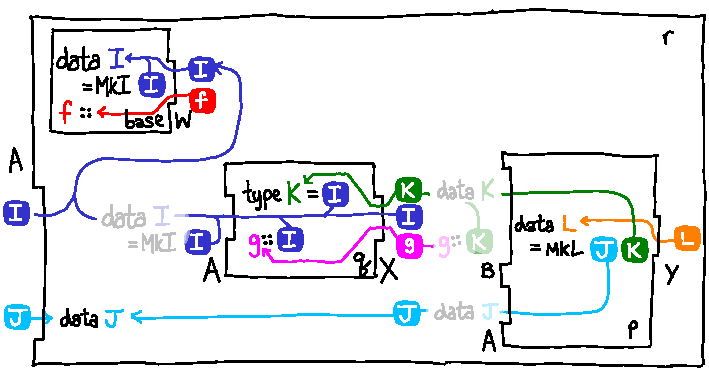
\includegraphics{figures/pqr-type-diagram.pdf}
\caption{Pictorial depiction of the types in our running example
(\cref{fig:linked-example}), with all original names replaced with
pointers to the declaration of the semantic object.
Lightened declarations (seen to the left of the holes for \texttt{A} and
\texttt{B} in \texttt{q} and \texttt{p}) specify requirements which
were subsequently filled by instantiation or signature merging.}
\label{fig:typing-example-diagram}
\end{figure}

After mixin linking has produced a \unit{} definition from a \ccomp{}
definition, the component can now be \emph{typechecked}, producing \emph{module types}
which record the type information
of all top-level declarations in a module.
GHC Haskell's module types resemble Haskell source code,
with two differences:
first, all declarations have been annotated with full type and kind
information; second, all identifiers have been renamed into \emph{original
names} which identify the exact module which originally defined the
entity.  The types of our running example can be found
in \cref{fig:typing-example}; to see the full grammar for module
types skip ahead to \cref{fig:semantic-objects}.

In the rest of this section, we'll describe the interface and semantic
representations in more detail, and outline how each type of declaration
in a \unit{} can be typechecked.

\subsection{Typechecking a module}

A module is typechecked to produce a \emph{module
type}, consisting of an \emph{export
specification} (what gets brought into scope when
you import this module) and a set of \emph{defined entity specifications}
(the types and values defined by this module).

%   Syntactically, these are represented with
%   a notation reminiscent of Haskell module declarations:
%   $\UobjTau{\UNs}{\overline{\Uty}}$.

For example, the module
\modname{W} in \cidl{base} (\cref{fig:linked-example}) type
checks to the following module type (see also \cref{fig:typing-example}):

\begin{figure}[H]
\center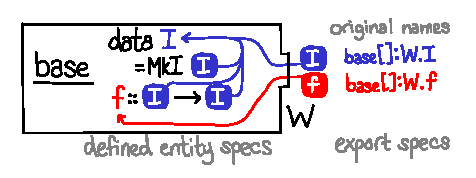
\includegraphics{figures/base-types.pdf}
\end{figure}

\noindent
In the diagram, we depicted the type of \verb|box| pictorially
by wiring up the enboxed references of \texttt{I} and \texttt{f} to their definitions.
The enboxed references \texttt{I} and \texttt{f} are
not unresolved Haskell-source level names,
but \emph{original names} $N ::=
M.n$, which serve as unique identifiers for any entities; in the
diagram, the original names have been abbreviated for concision.  An
original name for an entity defined in a module is generated by joining
the identity of the module that defines it---$\MOD{base}{}{W}$ in this
case--- with the Haskell source level name (e.g., \texttt{I},
\texttt{f}).
If, when typechecking another module, we need to look up the kind of
$\MOD{base}{}{W}.\texttt{I}$, we look up the module type of
$\MOD{base}{}{W}$ from the context and then find the defined entity
specification for \texttt{I} within the module type.

\subsection{Typechecking a signature}

Typechecking \cidl{q} (\cref{fig:linked-example}) from our running example requires
us to deal with a signature declaration.  Here is a
representation of the final type of \cidl{q}:

\begin{figure}[H]
\center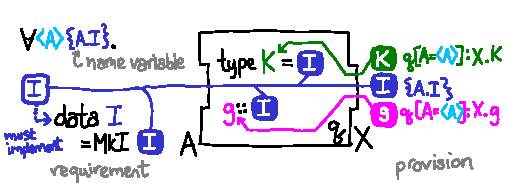
\includegraphics{figures/q-types.pdf}
\end{figure}

\noindent
In the diagram, the declarations from the signature are
drawn externally from \cidl{q}.  We do not know what module
will be used to fill the requirement \texttt{A}, and
consequently, we don't know what original name will provide an
implementation of \texttt{I}, although we do have a declarative
specification which any implementation must satisfy.  When we type check against the
signature, we use this required declaration ``as if'' it were
a declaration of its own.

In mixin linking, we bound a module variable \hv{A} to represent the
unknown module identifier.  In typechecking, we bind a \emph{name
variable} $\nhv{m.n}$ to represent the unknown entity $n$ required by
requirement $m$.
You may be wondering why name variables are not simply defined as
$\hv{m}.n$.  Read literally, names of this form demand that $n$ be defined
by $\hv{A}$ itself, ruling out the possibility that it \emph{reexports}
$n$ from another module.

In the diagram above, the results of typechecking the module \texttt{X}
are also shown.  As before, entities that are defined in the module
are given original names combining the module identifier (\MOD{q}{\subst{A}{\hv{A}}}{X})
and their source level name, while reexported entities retain the original
name of their source.

\subsection{Typechecking a dependency}

Now we can define the key operation for typechecking in \Backpack{}:
how to compute the type of \cidl{q} instantiated with an implementation
for its requirements.  These instantiations are specified to the
compiler via \texttt{dependency} declarations.
Let's first consider a simple one: filling \cidl{q}'s
requirement with \modname{W} from \cidl{base}, i.e., $\UsynDepEmpty{\cidl{q}[\subst{A}{\Mod{\cidl{base}[]}{W}}]}$.

\begin{figure}[H]
\center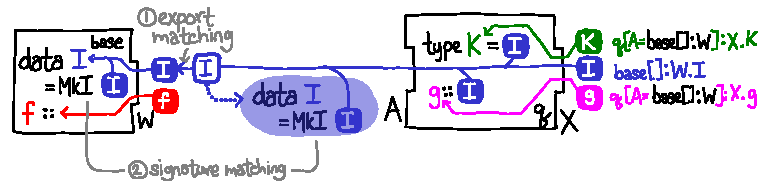
\includegraphics{figures/base-q-types.pdf}
\end{figure}

\noindent There are two key steps. First, we take the
required export specification from \cidl{q}, and the provided export
specification from \cidl{base}, and we perform \emph{export matching},
matching every required entity with an exported entity with the same
name from the implementing module.  In our example, we learn that
\nhv{A.I} is instantiated with \MOD{base}{}{W}.\texttt{I}; in the graph
representation, all previous references to \nhv{A.I} are rewritten so
that they now point to the declaration for \MOD{base}{}{W}.\texttt{I}.
Additionally, we must apply the module substitution to the original names of all
entities defined in the instantiated component: e.g., we apply the
substitution $\subst{A}{\Mod{\cidl{base}[]}{W}}$ to the original name
\MOD{q}{\subst{A}{\hv{A}}}{X}.\texttt{K}.

When we do this, we must check if this instantiation is
well-typed via \emph{signature matching}: do the
declarations provided by \cidl{base} match the required declarations of
\cidl{q}?  This proceeds by comparing the declarations of each required
entity with the declaration of the corresponding provided entity.
In our example, the implementation of \texttt{I} is an algebraic data
type which matches the required declaration exactly; the implementation
would also have successfully matched an abstract data type \texttt{data I}.

It is important that export matching happen before
signature matching, as the process of export matching may reveal more
type equalities.  This can be seen in the instantiation of \cidl{p} in
our running example:

\begin{figure}[H]
\center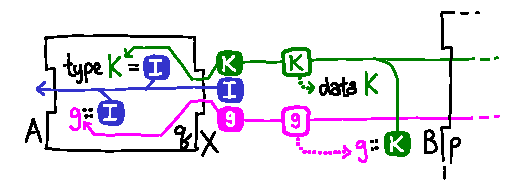
\includegraphics{figures/instantiation-with-synonyms.pdf}
\end{figure}

\noindent
In this example, it is not syntactically obvious that \verb|g :: I|
and \verb|g :: K| are matching declarations.  \verb|I|
and \verb|K| are definitionally equal because the abstract data type \verb|K|
was implemented by the type synonym \verb|type K = I|:

\begin{figure}[H]
\center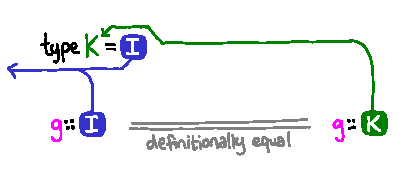
\includegraphics{figures/instantiation-with-synonyms-reduced.pdf}
\end{figure}

\noindent
By wiring up everything beforehand, we ensure that signature matching
sees the correct equalities.

%   This does mean that we may construct some
%   types in the graph representation that are ill-kinded before discovering
%   that signature matching fails!

\subsection{Signature merging}
\label{sec:signature-merging}

The distinguishing characteristic of mixin
linking is not just the linking that occurs when a module is brought into
scope with the same name as a signature, but also the \emph{signature merging}
that occurs when two signatures are brought into scope under the same name.
Like dependency instantiation, we must take the required exports of each
signature being merged and merge them with the identically
named entities from other signatures.

%   Unlike dependency instantiation,
%   this matching process is \emph{bidirectional}, as can be seen in the

The subtlety of signature merging is determining whether or not the declarations
of a type in two signatures are compatible with one another.  Consider
the following example (which is adapted from the MixML paper~\cite{rossberg+:mixml}):

\begin{tabular}{p{0.45\textwidth} p{0.45\textwidth}}
\begin{lstlisting}
signature A where
    type T = Int
    data U
    f :: Int -> U
\end{lstlisting}
&
\begin{lstlisting}
signature A where
    data T
    type U = Bool
    f :: T -> Bool
\end{lstlisting}
\end{tabular}

\noindent
It is not obvious that \verb|Int -> U| has the same type as \verb|T -> Bool|,
unless we refine \verb|U| to \verb|Bool| and \verb|T| to \verb|Int| in
both signatures.

\begin{figure}[H]
\center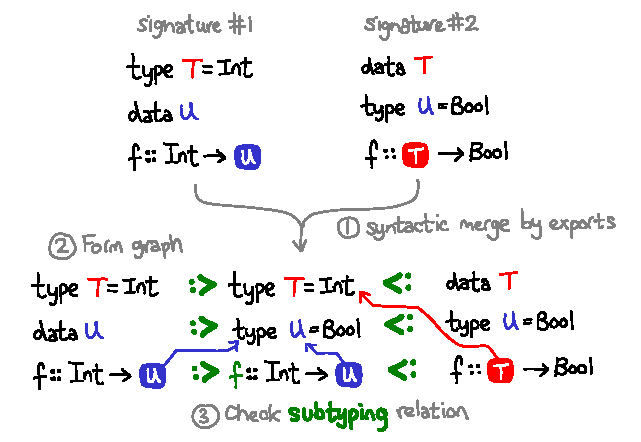
\includegraphics{figures/signature-merging.pdf}
\end{figure}

\noindent
To merge these signatures,
we first take the required export specifications from each signature and
match entities which have the same names.
For every entity which occurs in multiple signatures,
we pick out the most-defined
declaration from each signature.  In this example, the choice is easy:
\verb|type T = Int| is more defined than the abstract \verb|data T|,
so we pick it for the merged signature.
If there is not a unique choice, we pick an arbitrary one; we will
subsequently check that all of the entities are equivalent.\footnote{You might
wonder why we cannot designate a specific entity to use.  Because
signature merging is unordered, the only way to treat signatures equally
would be to define some merging operation on them.  However, this is
technically challenging to do, as we do not yet know what the refined
types of the entities are.  Picking an arbitrary entity cuts the
gordian knot, while only introducing nondeterminism in a benign way.}

Then, we check if each of the original declarations are compatible with
the merged declaration.  The important twist is that whenever we
see a name in one of the original declarations, we must resolve it
to its definition in the \emph{merged} signature: in the diagram above,
this is depicted by pointing the enboxed references to the central
declarations.  Now we can see that both instances of \verb|f| have a type that
is definitionally equal to \verb|Int -> U|.

%   \paragraph{Signature merging}
%   There is one final detail: how to merge requirements from
%   the dependencies of a component.  If
%   we know the required module types of all our dependencies, the merge is
%   straightforward.  For example, here are the module types to be merged
%   in \cidl{r} for the signature \modname{A}:
%   \[
%   \begin{array}{lll}
%   &\begin{array}{l}
%       \UobjIface\: (\MOD{base}{}{W}.\texttt{I}) \\
%   \end{array} & \text{Local signature} \\
%   \oplus&
%   \begin{array}{l}
%       \UobjIface\: (\nhv{\texttt{A.J}}) \\
%       \quad\texttt{data J :: *}
%   \end{array} & \text{From \cidl{p}} \\
%   \oplus&
%   \begin{array}{l}
%       \UobjIface\: (\nhv{\texttt{A.I}}) \\
%       \quad\texttt{data I :: * = MkI}\ \nhv{\texttt{A.I}}
%   \end{array} & \text{From \cidl{q}} \\
%   =&
%   \begin{array}{l}
%       \UobjIface\: (\MOD{base}{}{W}.\texttt{I}, \nhv{\texttt{A.J}}) \\
%       \quad\texttt{data J :: *}
%   \end{array} & \text{Final requirement for \cidl{r}}
%   \end{array}
%   \]
%   %
%   The export lists are unioned together, and we discover that \nhv{A.I}
%   actually must implemented with $\MOD{base}{}{W}.\texttt{I}$. And since
%   the entity \texttt{I} is already implemented, we additionally
%   drop its specification from the resulting requirement (having checked
%   that its specification from \MOD{base}{}{W} matches that from \cidl{q}).

%   Unfortunately, this definition of signature merging is circular: to
%   compute the instantiated type of a component, we need to know the (full)
%   types of our requirements; but to compute the type of a merged
%   requirement, we need to compute the instantiated types of the components
%   which merge into the requirement. \Scott{I'm not sure what this means. Can
%   you identify how the problem manifests in the example so far?}
%   The solution to this problem is to
%   define \emph{partial instantiation}, which only instantiates a component
%   type as much as is necessary to determine the type of the requirement in
%   question.  We give the technical details in \cref{sec:compiler}.

%   \paragraph{Compiling instantiated components}
%   \Red{Need to rewrite this section, motivate why the semantics split
%   into separate type checking and compiler.}
%   When a \unit{} has no
%   requirements, it can be compiled.  In this case, compilation is very
%   trivial: the dependencies of \unit{}s can be successively instantiated
%   by Cabal to form a graph of instantiated components, which GHC can
%   simply compile in order.  In this way, the soundness of Haskell with \Backpack{}
%   trivially reduces to the soundness of Haskell without \Backpack{}.

%   While compilation of \Backpack{} is trivially sound, we would like to
%   relate type checking and compilation with a property that says that if a
%   unit typechecks compositionally, it also typechecks monolithically
%   (i.e., when you re-typecheck the entire transitive closure.)
%   Unfortunately, in full Haskell it is impossible for this to be the case
%   with our current signature language and semantics.  In Section \Red{XXX}
%   we give some examples and conjecture under what circumstances this
%   property does hold.


\section{Instantiation and compilation}
\label{sec:overview-instantiate}

Typechecking is all very well and good, but what about
running our programs?  For both soundness reasons (\cref{sec:limitations})
and performance reasons, it is desirable to defer compiling
until we know how all the requirements of a component are to be
filled.

When we have a \unit{} which has no unfilled requirements,
the package manager computes the
\emph{instantiated component graph}, reflecting all of the
concrete code dependencies of the component.  Specifically, given a closed instantiated component identity $p[S]$, for every
\texttt{dependency} $P$ of $p$'s mixed component, recursively
instantiate $\substw{P}{S}$ ($P$ after applying the $S$
substitution).  Furthermore, for every $\substMod{m}{P}{m'} \in S$,
recursively instantiate $P$.  Then, we compile each instantiated component
in topological order.  This compilation is exactly like ordinary
compilation without \Backpack. The only new feature is that signatures
compile into trivial modules which reexport entities from
the backing implementation; otherwise, modules that imported the signature might see
entities from the backing implementation that were not exported by the
signature.

It is important that the package manager computes
the instantiated component graph: \emph{applicative}
semantics of instantiation mean that completely independent
components could instantiate a library in the same way: in such
cases we should share the compiled code.  A traditional compiler cannot
do this: it is solely responsible for transforming source
files into object code.











%%% Local Variables:
%%% mode: latex
%%% TeX-master: "paper"
%%% End:

\chapter{\Uid{}s}
\label{sec:uid}

\begin{figure}[H]
\center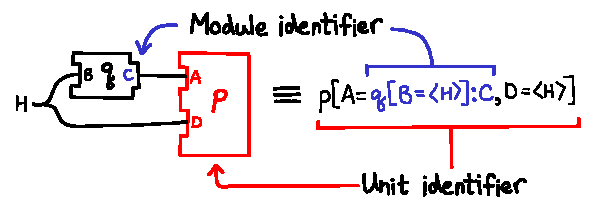
\includegraphics{figures/unit-identifier.pdf}
\end{figure}

At the core of Backpack is the expression language of \uid{}s.  A \uid{}
can be thought of in two ways:

\begin{enumerate}
\item A \uid{} is an \emph{expression} in the language of
   applicative functor applications, specifying how a
   library is instantiated.  Thus, we interpret $\uidl{p}{\substMod{A}{\cidl{q}}{B}}$
   as saying that $\cidl{p}$ is applied with \Mod{\cidl{q}}{B} at its hole (argument) \modname{A}.
%  (This is not entirely accurate in the presence of signature merging,
%  but it is a pretty good approximation).

\item A \uid{} uniquely \emph{identifies} a library: if
   two instances of a library are instantiated in the same
   way, they have equal unit identifiers, provide the same types and will be compiled
   and installed only once in the package database.
\end{enumerate}
%
In \Backpack{}, \uid{}s are a concept that is universal across the
package manager and compiler divide: mixin linking determines the \uid{}s of
the libraries that are in scope; the compiler subsequently consumes
these \uid{}s to determine what modules are in scope for import and what
requirements are inherited.  \Uid{}s are not intended to be written by
hand, although they are the basis for type equality and thus need to be
understood to some degree.

\Backpack{}'s \uid{}s are distinguished from \OldBackpack{}'s module
identities, as they operate on a per-library rather than per-module
basis.  This change in semantics was motivated in the desire for
unit identifiers for libraries to be computable without referring to
source code (which a per-module scheme like \OldBackpack{}'s requires).

In this chapter, we develop some basic metatheory on \uid{}s, giving
some graphical intuition for them as well as describing an unimplemented
extension to recursive \uid{}s.

\section{Syntax}

Here is the syntax of \uid{}s, recapitulated from Figure~\ref{fig:lcomponents}.

\[ \DIGatoms{} \]
\[ \DIGuid{} \]

\noindent
We fix a set of \emph{\cid{}s} and \emph{module names}, which serve as
labels to identify libraries prior to instantiation and the modules
within them, respectively. \Cid{}s are allocated by the
package manager after dependency solving and componentization and
generally encode the source package name, version, and transitive
dependency structure.

A \uid{} identifies a library (specified by a \cid{}) and a and how each
of its holes is to be filled (specified by a \emph{module
substitution}). A module substitution is a mapping from module name to
\emph{module identifier}, which specifies a particular module name from
an instantiated component (specified by a unit identifier), or a hole
module (indicating that the module is uninstantiated). Each module name
key of the substitution must be distinct.

%   In our concrete syntax,
%   these entries are given canonically in lexicographically sorted
%   order.

\section{Pictorial interpretation}

One way to understand unit identifiers is to visualize a graph of
component boxes:

\begin{figure}[H]
\center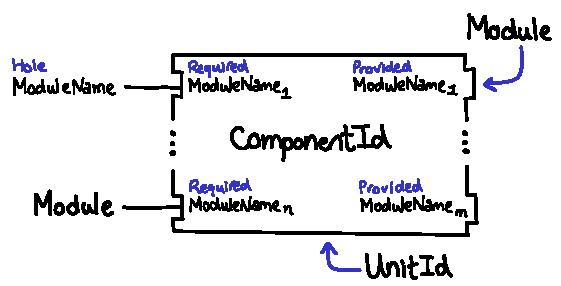
\includegraphics{figures/unit-identifier-pictorial.pdf}
\end{figure}

\noindent
Each component box is labelled with a component identifier and has a
series of input ports (on the left) and output ports (on the right). The
input ports represent all of the required module names of the component,
while the output ports signify a subset of the provided modules from
this component (output ports can be elided if they are unused). An
output port can be wired up to an input port to indicate the module is
being used to instantiate the requirement; if a ``hole'' module name is
wired to an input port, it indicates that this port is uninstantiated.
In our implementation of \Backpack{}, component graphs are acyclic
(but see Section~\ref{sec:recursive-uids} for the cyclic extension).

A unit identifier represents a specific box in a component graph, while
a module identifier represents a specific output port on one of these
boxes. It is worth emphasizing that the inputs to a component box
determine its identity: for example, the component box for a component
identifier can appear multiple times with different inputs.

Since \Backpack{} is an \emph{applicative} module system (functor
application is not generative), we can de-duplicate component boxes which
have the same component identifier and input modules, or (in reverse)
duplicate a component box and all of its inputs into two identical
graphs; in all of these cases, the diagrams represent multiple \uid{}s
which share common sub-expressions.  For example, the following
two diagrams are equivalent.

\begin{figure}[H]
\center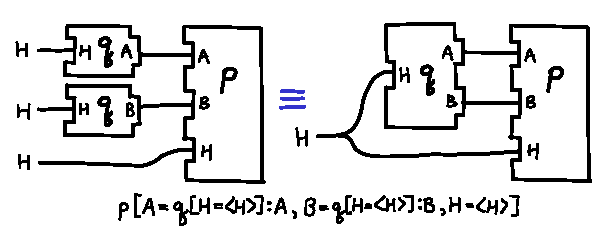
\includegraphics{figures/unit-identifier-pictorial-equivalence-example-2.pdf}
\end{figure}

The most expanded representation is always a tree of component boxes, each
with only a single output port; this representation corresponds exactly
to the abstract syntax tree of unit identifiers:

\begin{figure}[H]
\center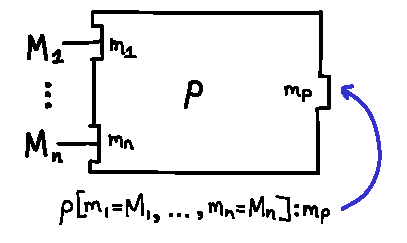
\includegraphics{figures/module-identifier-pictorial.pdf}
\end{figure}

\section{Substitutions}

Module substitutions can be applied to both unit and module identifiers, treating hole
modules as variables:

\[
\begin{array}{rcl}
  \substw{(\icid{p}{S})}{S'} &=_P& \icid{p}{\substw{S}{S'}} \\
  \\
  \substw{\holevar{m}}{\cdot} &=_M& \holevar{m} \\
  \substw{\holevar{m}}{\subst{m}{M}, S} &=_M& M \\
  \substw{\holevar{m}}{\subst{m'}{M}, S} &=_M& \substw{\holevar{m}}{S} \quad (m \neq m') \\
  \substw{(\Mod{P}{m})}{S} &=_M& \Mod{\substw{P}{S}}{m} \\
  \\
  \substw{(\overline{\subst{m}{M}})}{S} &=_{S}& \overline{\subst{m}{\substw{M}{S}}} \\
\end{array}
\]

\noindent
Pictorially, substitution plugs a component into an unfilled
hole module:

\begin{figure}[H]
\center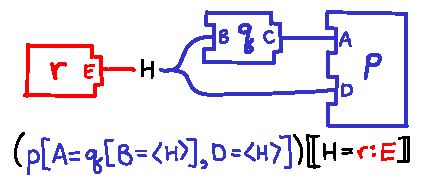
\includegraphics{figures/substitution-pictorial-example.pdf}
\end{figure}


%!TEX root = paper.tex
\chapter{Mixin linking} %  to the \ir{}
\label{sec:mix-in}

\begin{figure}[H]
\center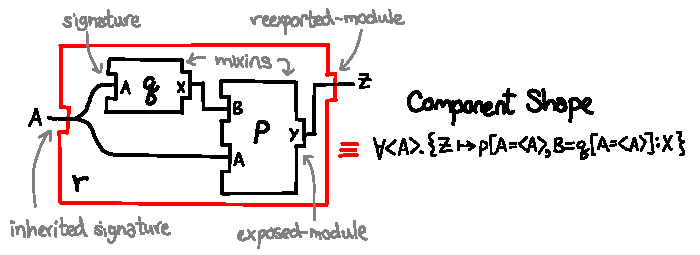
\includegraphics{figures/library-shape-overview.pdf}
\end{figure}

We now formalize mixin linking and describe some of its properties.
In particular, we define two major operations
on component shapes: $\textsf{link}()$, which wires up the components in
two shapes, and $\textsf{rnthin}()$, which thins and renames the input
and output ports of a shape; then, we say how to mixin link a
\ccomp{}.  For an informal description of mixin linking refer
to \cref{sec:overview-mixin}.

\[
\begin{array}{ll}
\DIGresolved{}
&
\begin{array}{l}
\DIGmixed{} \\
\DIGshape{}
\end{array}
\end{array}
\]

% Deferred reporting
% Correct rules for unification

\section{Pictorial interpretation}

We can build upon our graphical language of \uid{}s to specify a graphical
language of \emph{component shapes}, which we used in \cref{sec:overview-mixin}
to informally describe the mixin linking process.  A component shape is simply
a ``bigger box'' which contains some number of \uid{}s:

\begin{figure}[H]
\center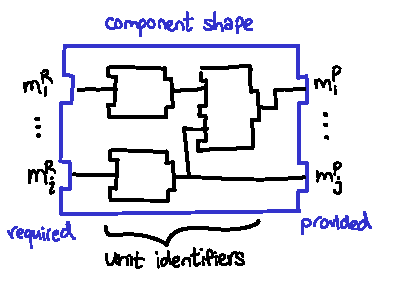
\includegraphics{figures/library-shape-blueprint.pdf}
\end{figure}

\noindent
The required module variables $\reqs = \overline{\hv{m^R_i}}$ can be
read off the diagram by taking the module names of the input ports,
while the provided modules $\provs = \overline{m^P_j \mapsto M_j}$ are a mapping from the module name of each output port to the module identity that is wired to
that port.

These diagrams must obey three rules:

\begin{enumerate}
    \item A wire from a input port cannot go straight to an output port; there
          must be an intervening \uid{}.
    \item No two ports (input or output) can have the same module name.
    \item Every unfilled requirement of a \uid{} must be propagated to the
          requirements of the enclosing component shape.
\end{enumerate}
%
We can restate these rules syntactically:

\begin{definition}[Well-formedness of component shapes] \normalfont{}
A shape $\lctxpair{\provs}{\reqs}$ is \emph{well-formed} if:
\begin{enumerate}
\item It does not provide module variables
(there is no $m$ such that $\hv{m} \in \textsf{range}(\provs)$),
e.g., $\lctxpair{\{\prov{B}{\hv{A}}\}}{\hv{A}}$ is ill-formed,
\item It does not require what it provides (no $m$
s.t. $\hv{m} \in \reqs$ and $m \in \textsf{dom}(\provs)$),
e.g., $\lctxpair{\{\prov{A}{\MOD{p}{}{A}}\}}{\hv{A}}$ is ill-formed,
\item It is closed; e.g.,
$\lctxpair{\{\prov{B}{\MOD{p}{\subst{A}{\hv{C}}}{B}}\}}{\hv{A}}$ is ill-formed.
\end{enumerate}
\end{definition}

\noindent
Occasionally, we may draw a \uid{} with multiple ports as a shorthand
for two module identifiers which share a \uid{}; although the resulting
box looks similar to a component shape, it is less expressive, since a
component shape can have \emph{different} unit identifiers for the
modules it provides (as can be seen in the above example).

\section{Linking component shapes}

In our informal description of mixin linking, we simply described mixin
linking as simply ``wiring up'' the input output ports of components;
this wiring operation corresponds to unification in the syntactic realm.

Although the intuitive description of mixin linking is very simple,
there is one subtlety: what happens if two modules (not
signatures) are brought into scope with the same name?  Naively,
we should \emph{unify} the two module identities, erroring if they
have incompatible module identities.  But there are two problems
with this approach:

\begin{enumerate}
    \item If two distinct modules are brought into scope with the same
    name, but are never used (in particular, if they are not used to
    fill a signature), it is better not to report an error if they do
    not unify.  This is inline with Cabal's existing behavior, and is
    analogous to Haskell's name resolution rules, which only report an
    ambiguity when the ambiguous name is used.

    \item Suppose that $\Mod{\cidl{q}[\subst{A}{\hv{A}}]}{X}$ and
        $\Mod{\cidl{q}[\subst{A}{\Mod{\cidl{a}}{A}}]}{X}$ are in
        scope at the same name, and we need to use them
        to fill a requirement (so that case (1) does not apply).
        If we set $\subst{A}{\Mod{\cidl{a}}{X}}$,
        the two modules unify.  But unifying in this way has a surprising consequence:
        it means that one cannot determine the new set of
        required module names by taking the set difference of the
        required and provided names in scope: a unification between
        two module identities can cause other requirements to be filled.
        We think it is better to request that users explicitly fill all
        requirements via mixin linking.

\end{enumerate}
%
Thus, we have two goals:

\begin{itemize}
    \item If two distinct modules are brought into the scope with the same
    name, but are never used, this should not be an error.

    \item Mixin linking should be order-invariant, as the source language
    is unordered.
\end{itemize}
%
To handle these problems, we introduce the concept of
\emph{provided module sets} $\Pi ::= \overline{m \mapsto \overline{M}}$,
which is a mapping from module names to sets of module identities
(as opposed to a single module identity, as is the case for a component shape).
We define two operations on provided module sets:

\begin{itemize}
\item Any set of provided modules $\provs$ can be injected into provided module sets $\Pi$ by taking $\Pi(m) = \{ \provs(m) \}$ for all $m \in \dom(\provs)$.

\item Provided module sets can be merged pointwise: $\bigoplus_i \Pi_i = \Pi$ where $\dom(\Pi) = \bigcup_i \dom(\Pi_i) \land\forall m \in \dom(\Pi).\, \Pi(m) = \bigcup_i \Pi'_i(m)$, where $\Pi'_i(m) = \Pi_i(m)$ when $m \in \dom(\Pi_i)$, and $\Pi'_i(m) = \varnothing$ otherwise.
\end{itemize}
%
We now define an $n$-ary linking operation on sets of component shapes: $\textsf{link}(\overline{\lctxpair{\provs_i}{\reqs_i}})$, which produces a substitution and a new component shape as follows:

\begin{enumerate}
    \item Let the provided module sets of all shapes be $\Pi = \bigoplus \provs_i$.
    \item Let the required module variables be $\reqs_\mathsf{all} = \bigcup \reqs_i$.
    \item The requirements which are filled are $\reqs_\mathsf{filled} = \reqs_\mathsf{all} \cap \dom(\Pi)$.
    \item For each $m_i \in \reqs_\mathsf{filled}$, unify $\hv{m_i}$ with each module identity in $\Pi(m_i)$.  (Thus, provided modules which are not used remain ununified.)  Let the overall substitution produced be $S$.
    \item The remaining requirements are $\reqs = \reqs_\mathsf{all} - \reqs_\mathsf{filled}$.  Check that $\substw{\reqs}{S} = \reqs$ (unification did not cause a requirement to be implicitly filled).
    \item Let $\provs(m) = \Pi(m)$ for all $m$ such that $\Pi(m) = \{ M \}$ for some $M$ (i.e., take the singleton module sets).
    \item Return new substitution $S$, and new shape $\lctxpair{\provs}{\reqs}$
\end{enumerate}
%
\paragraph{A little design discussion} Unfortunately, this merging operation is not compositional (i.e., cannot be decomposed into a series of binary merge operations); consider the
merge of these shapes: (1) $\lctxpair{ \prov{A}{\MOD{p}{\subst{H}{\hv{H}}}{A}} }{ \hv{H} }$,
(2) \prov{A}{\MOD{p}{\subst{H}{\MOD{q}{}{H}}}{A}}, (3) $\lctxpair{\varnothing}{\hv{A}}$
and (4) \prov{H}{\MOD{q}{}{H}}.
Shapes 1--3 cannot merge together by themselves (we can unify
the \modname{A}s, but as \modname{H} is never
filled we reject the shape in step (5)). Merging these shapes simulateously
with shape 4 solves this problem.

There are a few obvious alternative designs which do not work.
We cannot say that the result of unifying shapes 1--2 is shape 2 (i.e.,
\modname{H} is filled due to the unification of \modname{A}), because
then we would then allow a merge with the shape \prov{H}{\MOD{q}{}{H2}} (call this
shape 4'),
whereas if shape 1 merged with shape 4' first, the identity at \modname{A} would refine
to one that was incompatible with shape 2.

One alternative design that does work and is compositional is to associate a
component shapes with a context which accumulates constraints on module
holes which were not otherwise filled.  When the hole is eventually filled
by a proper requirement, we check that those constraints are satisfied.
But in the end, we probably would like to enforce that all constraints are
discharged when computing a final component shape, at which point the algorithm
ends up being the same as the $n$-ary variant above.

\section{Thinning and renaming component shapes}

%   There is an interesting counterexample showing that linking is not
%   associative:

%   \begin{enumerate}
%   \item $\{ \prov{A}{\cidl{p}[]} \}$
%   \item $\lctxpair{ \prov{B}{\Mod{\cidl{q}[\subst{A}{\hv{A}}]}{B}}, \prov{C}{\Mod{\cidl{q}[\subst{A}{\hv{A}}]}}{C} }{\hv{A}}$
%   \item $\{ \prov{B}{\Mod{\cidl{q}[\subst{A}{\cidl{p}[]}]}{B}} \}$
%   \end{enumerate}

%   Linking (1) and (2), and then (3) works, but linking (2) and (3) does
%   not, as the provisions are required to 

\begin{definition}[Thinning and renaming component shapes] \normalfont{}
We define $\textsf{rnthin}$ on a shape $\lctx$, a total
module renaming $r_R$ and a partial module renaming $r_P$ as follows:
\label{def:rnthin}
  \[
  \begin{array}{l@{\;\;=\;\;}l}
    \Frename{r_R}{\lctxpair{\provs}{\overline{\hv{m_i}}^i}}{r_P}
    % \substw{\substw{r_P^{-1}}{\provs}}{r_R}
    & \lctxpairx%
        {\overlinej{\prov{r_P(m'_j)}{\substw{\provs(m'_j)}{r_R}}}}
        {\overlinei{\holevar{r_R(m_i)}}} \\
    \multicolumn{2}{l}{\quad \textsf{where}~\textsf{dom}(r_P) = \overlinej{m'_j} } \\
  \end{array}
  \]
\end{definition}
%
Intuitively, $r_R$ applies a renaming on all of the input ports of
the component shape, while $r_P$ applies a renaming on the output ports
of a component shape.  $r_R$ must be total because we are not allowed
to ``drop'' any requirements; furthermore when we rename a requirement
we must also rename each reference to it in the provided $M$s.  $r_P$
does not have to be total, and the resulting output ports of the
component shape will only be those mentioned in $r_P$.

For example, if you have a component shaped
$\lctxpairx{\provMOD{A}{p}{\subst{A}{\holevar{B}}}{A},
\provMOD{C}{q}{}{C} }{\modname{B}}$ and you apply the renaming
$(\Sas{A}{X})$ $\texttt{requires}$ $(\Sas{B}{Y})$, we should get a new shape
$\lctxpairx{\provMOD{X}{p}{\subst{A}{\holevar{Y}}}{A}}{\modname{Y}}$.

\begin{figure}[H]
\center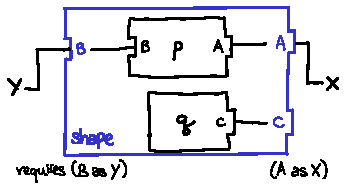
\includegraphics{figures/mixin-renaming-ex.pdf}
\end{figure}

\section{Component mixin linking}

\begin{figure}


\fbox{$\shctx \vdash \Scomp \leadsto \Uunit \haspr \lctx$}

\[
\frac{
\begin{array}{c}
  % \prereqs = \Freqs{\mathtt{component}\: p\: \{ \overline{I_i}^i; \overline{D_j}^j \}} \qquad
  % P = p(\prereqs) \\
  P = p[\reqs] \qquad
  \forall i:\; \shctx; P \vdash \Sdecl_i \leadsto \Uudecl_i \haspr \lctx_i \\
  (S, \lctx) = \Flink{\overlinei{\lctx_i}} \qquad
  \lctxpair{\provs}{\reqs} = \lctx \qquad
  % \provs = \{\overlinej{m_j \mapsto M_j}\}\qquad
  r_P = \overlinei{\Fprovs{\Sdecl_i}} \\
\end{array}
}{
  \shctx \vdash \Scomponent{p}{\overlinei{\Sdecl_i}}
    \leadsto \UsynUnit{p}{\reqs}{\overlinei{\substw{\Uudecl_i}{S}}}
    \haspr \Frename{\,\cdot\,}{\lctx}{r_P}
}
\]
\\


\fbox{$\shctx; P \vdash \Sdecl \leadsto \Uudecl \haspr \lctx$}

%   \[
%   \begin{array}{rcll}
%   &\vdash_\mathsf{ex}& \verb|exposed-module|\: m &\Rightarrow (m, m) \\
%   &\vdash_\mathsf{ex}& \verb|reexported-module|\: m_0\: \mathtt{as}\: m &\Rightarrow (m_0, m) \\
%   \end{array}
%   \]
\[
\frac{
p \haspr \lctx \in \Delta \qquad
\lctx = \lctxpair{\provs}{\reqs} \qquad
(r_R, r_P) = \textsf{getrns}(\lctx, \I{rns}) \qquad
\lctx' = \Frename{r_R}{\lctx}{r_P}
}{
\shctx; P \vdash\Sinclude{p}{\I{rns}} \leadsto \UsynDep{p[r_R]}{r_P} \haspr \lctx'
}
\]
\[
\begin{array}{ll@{\;\;}llll}
  \shctx; P &\vdash&\Sexposed{m}{\Uhsbody} &\leadsto
    & \UsynMod{m}{\Uhsbody} &\;\;\haspr\;\; \{\provMod{m}{P}{m}\} \\
  \shctx; P &\vdash&\Sother{m}{\Uhsbody} &\leadsto
    & \UsynMod{m}{\Uhsbody} &\;\;\haspr\;\; \{\provMod{m}{P}{m}\} \\
  \shctx; P &\vdash&\Srequired{m}{\Uhssig} &\leadsto
    & \UsynSig{m}{\Uhssig} &\;\;\haspr\;\; \lctxpairx{\shnull}{\hv{m}} \\
  \shctx; P &\vdash&\Sreexported{m}{m'} &\leadsto
    & \varnothing &\;\;\haspr\;\; \{\} \\
\end{array}
\]
\caption{Component mixin linking. We implicitly lift $\Theta = \overline{\protect\hv{m}}$
into a substitution $\overline{\protect\subst{m}{\protect\hv{m}}}$.}
\label{fig:mix-in}
\end{figure}

Given $\textsf{link}()$ and $\textsf{rnthin}()$, we are well equipped to say how to mixin link
an entire \ccomp{} (\cref{fig:mix-in}).  Our general strategy will be to compute the
component shape of every $\I{rdecl}$ (as well as its elaboration to
$\mdecl$) and link them all together in the component judgment,
combining all of the $\mdecl$s together to form the final
elaborated \unit{}.  There is an auxiliary definition (Definition~\ref{def:provs})
which computes the final renaming on the provisions of the
component, so that only \texttt{exposed-module}s and \texttt{reexported-modules}
are exposed to the world.

The rules for shaping modules and signatures are straightforward: a
module $m$ provides the module identity $\Mod{P}{m}$, where $P$ is the
component identity of the component currently being shaped; a signature
$m$ adds a requirement $\hv{m}$.  The rule for includes is more
interesting: we look up the shape of the included unit from the context ($\shctx$),
and then rename it according to the user provided renamings $\I{rns}$.
There is an auxiliary definition (Definition~\ref{def:getrns}) for
translating renaming syntax into a pair of module renamings.

Our presentation of the judgment is slightly
nondeterministic in that it assumes we know the set of requirements
$\Theta$ upfront to compute $P$; however it's easy to see that $P$ is
only used for the module identities assigned to module declarations, and
thus does not actually affect the final requirements of a component.
In practice, $\Theta$ might be computed by a pre-shaping pass.

\begin{definition}[Interpretation of thinning and renaming] \normalfont{}
\label{def:getrns}
\[
  \begin{array}{l@{\;\;=\;\;}l}
    \textsf{getrns}(\lctxpair{\provs}{\reqs}, [\Slparen\overline{\I{rn}_P}\Srparen]~[\texttt{requires}~ \Slparen\overline{\I{rn}_R}\Srparen])
    & (r_P, r_R)
  \end{array}
\]
The syntactic \texttt{include} declaration specifies renamings for
provisions and requirements, but users are allowed to omit a renaming
altogether (in which case everything is brought into scope) or give
only a partial requirement renaming (in which case the requirement
renaming is extended to be total over $\reqs$).
\textsf{getrns} simply computes the appropriate $r_R$ and $r_P$
given this syntax.
\end{definition}

\begin{definition}[Interpretation of exposed/reexported modules] \normalfont{}
\label{def:provs}
\[
  \begin{array}{l@{\quad=\quad}l}
    \Fprovs{\Sexposed{m}{\_}} & \prov{m}{m} \\
    \Fprovs{\Sreexported{m}{m'}} & \prov{m}{m'} \\
    \Fprovs{\_} & \cdot \\
  \end{array}
\]
Only modules specified with \texttt{exposed-module} or
\texttt{reexported-\allowbreak{}module} should be put in the final shape of
a component.  \textsf{provs} computes the appropriate $r_P$ based
on these declarations.
\end{definition}

%!TEX root = paper.tex
\chapter{Type checking}
\label{sec:compiler}

We now give a formal model of the type checking process on mixed
units.  This is challenging, as GHC Haskell's type system is quite
complex, and a full formalization of all aspects of GHC Haskell is
beyond the scope of this thesis.

Here is a summary of what will be covered in this chapter:

\begin{itemize}
\item We will specify a language of semantic
objects (Section~\ref{sec:semantic-objects}) that covers the most
important source level constructs supported by Haskell today (including
type families and type classes) but leave some aspects of the semantic
objects unspecified when \Backpack{} does not rely on them in an important
way.
\item We'll formalize how type lookup operates during type checking (Section~\ref{sec:typing/lookup}),
but not specify the overall process of typechecking modules and signatures are actually typechecked. (Section~\ref{sec:typing-haskell})
\item We describe the top-level process of typechecking a mixed component (Section~\ref{sec:typing/main}), which extends GHC Haskell's existing typechecking process with checks for dependency well-typedness and signature typechecking.
\item Finally, we describe the subtyping (Section~\ref{sec:subtyping}) and merging (Section~\ref{sec:typing/merging}) relations, which specify precisely under what situations does a module implement a signature and the semantics of signature merging.  We will also develop some basic metatheory relating subtyping and merging (merging is the greatest lower bound on the subtyping relation).
\end{itemize}

%   It's not possible to
%   give a full semantics, since that would involve formalizing all of
%   Haskell as implemented by GHC, but we will informally explain the
%   operation of the judgments we assume are given to us.

\section{Semantic objects}
\label{sec:semantic-objects}

\begin{figure}
\[ \DIGinterface{} \]
\caption{Semantic objects of GHC Haskell with \Backpack{}}
\label{fig:semantic-objects}
\end{figure}

The semantic objects of GHC Haskell, extended with \Backpack{}, are
given in Figure~\ref{fig:semantic-objects}.  These semantic objects
correspond closely to the top-level declarations supported by
Haskell's syntax, but with a few key differences: first, every
identifier is resolved to an \emph{original name} ($N$) which identifies
the exact module that holds the declaration describing this identifier;
second, all declarations are explicitly annotated with types ($\tau$), kinds ($\kappa$) and
roles ($\rho$).\footnote{Type families are not annotated with roles, because their
type parameters are always at nominal role.}  If the kinds or roles are not
relevant to a judgment, we may elide them.

The most important semantic object is the module type ($T$).  A module
type consists of four components:

\begin{enumerate}

    \item The export list ($\UNs ::= \overline{N}$), which
    specifies what entities are brought into scope when a module is
    imported.  Every original name in an export list has a unique
    occurrence name (e.g., $\UNs(n) = N$).

    \item The type declarations ($\Utys$), which give
    definitions for each entity provided by a module.  Every defined
    entity list defines a particular entity $n$ (shaded in gray
    in Figure~\ref{fig:semantic-objects}).  Like export lists,
    each declaration in a module has a unique occurrence name
    (e.g., $\Utys(n) = \Uty$).

    \item A set of instances ($\Uinsts$), which specifies the class
    and family instances defined in this module.

    \item The set of modules transitively imported by this module
    ($\Uimps$), which controls the set of \emph{orphan instances}
    (instances which may not necessarily be in scope) which are in scope
    when performing type class resolution.  If the module in question
    defines orphan instances, its identity is included in this list.

\end{enumerate}
%
Below is a simple example of a module's Haskell source code and its
corresponding module type:

\vspace{-1em}
\begin{figure}[H]
\centering
\begin{shortmath}
\begin{tabular}{p{0.30\textwidth} p{0.30\textwidth}}
\begin{lstlisting}
module A where
    data T = MkT
    f = MkT
    instance Eq T where
        MkT == MkT = True
\end{lstlisting}
&
\vspace{-12pt}
\[
\begin{array}{l}
    \UobjIface\: (\Mod{P_0}{A}.\texttt{T}, \Mod{P_0}{A}.\texttt{f}) \\
    \qquad\texttt{data T where MkT} :: \Mod{P_0}{A}.\texttt{T} \\
    \qquad\texttt{f} :: \Mod{P_0}{A}.\texttt{T} \\
    \qquad\texttt{instance} :: N_{Eq}~\Mod{P_0}{A}.\texttt{T} \\
\end{array}
\]
\end{tabular}
\end{shortmath}
\end{figure}

\vspace{-2em}
\noindent
Here, $P_0$ represents the unit identifier that this module was
being typechecked as a part of (for example, if \verb|module A| was
in the component \verb|p| with no holes, then $P_0 = \uidl{p}{}$),
and $N_\texttt{Eq}$ is the original name of the equality type
class (not shown, but part of Haskell's Prelude, a set of declarations
which are always in scope).

There are some slight differences with the module type of a signature:

\vspace{-1em}
\begin{figure}[H]
\centering
\begin{shortmath}
\begin{tabular}{p{0.30\textwidth} p{0.30\textwidth}}
\begin{lstlisting}
signature A where
    data T
    f :: T
\end{lstlisting}
&
\[
\begin{array}{l}
    \UobjIface\: (\nhv{A.T}, \nhv{A.f}) \\
    \qquad\texttt{data T} \\
    \qquad\texttt{f} :: \nhv{A.T}
\end{array}
\]
\end{tabular}
\end{shortmath}
\end{figure}

\vspace{-2em}
\noindent
Instead of original names based off of the ambient unit identifier $P_0$,
every defined entity is allocated a fresh name hole (e.g., $\nhv{A.T}$),
which may be subsequently substituted with the actual original name of the
implementing declaration.

A collection of module types forms a component ($\Xi$), where each module
type is annotated with a $+$ or $-$ to indicate if it is a module or
signature.   Although the syntax of component types suggests that a module
type can be put into the context at any name, a particular module
identity is baked into the module type (as can seen in the example
above); a module type must be placed in the context consistently with
the module identifier it was typechecked with.  (We could have avoided
this by applying a ``selfification'' step prior to adding
modules to the context, but the current presentation is more direct and
accurately describes how GHC is implemented.)

\section{Typing rules}

We organize our formalization of \Backpack{} typing into a few
concerns:

\begin{itemize}
    \item The assumed Haskell judgments (Figure~\ref{typing:haskell}) are the
        Haskell type-checking judgments we assume are available, but which
        we do not formalize.

    \item The top-level typing rules (Figure~\ref{typing:main}) tell us
        how to typecheck the declarations of a component and form the final
        component type.

    \item The type lookup and renaming rules (Figure~\ref{typing:lookup}) tell us how to
        get the type of a module by looking up the original type from
        the context, and then \emph{renaming} it according to the substitution
        recorded in the module identifier.

    \item The subtyping rules (Figures~\ref{typing:top-subtyping}--\ref{typing:subtyping})
        specify when one module type is a subtype of another, and is used
        by both signature merging and dependency matching.

    \item The merging rules (Figure~\ref{typing:merging}) specify how the
        module types are merged together during signature merging.

\end{itemize}
Most typing rules require the following three pieces of context:

\begin{itemize}
    \item The external component type context $\Gamma ::= \overline{p : \Xi}$,
        which records the types of all components we have previously
        typechecked.  These components are typed but not instantiated.
    \item The local type context $\Delta :: \overline{m : T^s}$,
        which records the types of the modules and signatures we have typechecked
        from the current package.
    \item The current unit identifier $P_0$, which identifies the component
        we are typechecking. It is used to generate the original names
        of declarations in modules and determine when a lookup should be
        done in the local type environment.
\end{itemize}
Some rules require some extra context:

\begin{itemize}
    \item The logical context $\mathcal{L} ::= \overline{m \mapsto M}$ specifies
        which module identity is brought into scope when a module name is imported.
        It is needed when typechecking unrenamed Haskell source code, but is
        otherwise not needed for typechecking.

    \item The shape context $\shctx ::= \overline{p : \lctx}$ specifies what
        module identities are provided by a package; this is used to resolve
        a list of \texttt{dependency} declarations into the logical context $\mathcal{L}$.
\end{itemize}

\subsection{Assumed Haskell judgments}
\label{sec:typing-haskell}

\input{typing/haskell}

We assume some judgments for various operations on
Haskell, which we do not formalize:

\begin{itemize}
    \item Module and signature typechecking are judgments which typecheck
    module (\I{hsmod}) and signature (\I{hssig}) source into module
    types.  Alongside the usual context, these judgments also require
    the logical context $\mathcal{L}$ so that they can resolve imports,
    and the name $m$ of the module they are typechecking (along with $P_0$,
    this will determine what original names of the declarations in
    the module and signatures will be: $\Mod{P_0}{m}.n$ in the case
    of a module, and $\nhv{m.n}$ in the case of a signature.)

    \item We also need judgments for testing type and kind equality.
    These require a context, because type synonyms and type families
    can introduce nontrivial definitional equalities between types that
    are syntactically dissimilar.

    \item Finally, we need a judgment for testing if a type class
    instance is derivable from the instances available in the context,
    plus some set of orphan instances (indicated by \I{orphs}).  Informally,
    this judgment collects all instances which are transitively reachable
    from \I{orphs}, as well as the modules which define all of the types
    mentioned in \I{inst}, and then runs the instance constraint solver
    to see if \I{inst} is implied by these instances.
\end{itemize}
%
%   We need these judgments to uphold some properties;
%   in particular, we require type and kind equality to be \emph{substitutable}:

%   \begin{axiom}[Type equality substitutability]
%   If $\ctx; \vdash \tau =_\textsf{hs} \tau'$,
%   then for any $\USn$, $\ctx; \vdash \substw{\tau}{\USn} =_\textsf{hs} \substw{\tau'}{\USn}$.
%   \end{axiom}

%   \begin{axiom}[Kind equality substitutability]
%   If $\ctx; \vdash \kappa =_\textsf{hs} \kappa'$,
%   then for any $\USn$, $\ctx; \vdash \substw{\kappa}{\USn} =_\textsf{hs} \substw{\kappa'}{\USn}$.
%   \end{axiom}

%   See Section~\ref{sec:substitutability} for more discussion on substitutability.

\subsection{Top-level typing rules}
\label{sec:typing/main}

\begin{figure}

\fbox{\textbf{Top-level typing:} $\shctx; \Gamma \vdash \mcomp : \Gamma$}

\[
\frac{
\begin{array}{c}
%\shctx \vdash \overline{\I{dep_i}} \leadsto (\mathcal{L}, \mathcal{D}) \qquad
\mathcal{L} = \bigoplus_i \textsf{exposes}(\shctx, P_i, r_i) \qquad
\mathcal{D} = \bigoplus_i \textsf{inherits}(P_i) \qquad
P_0 = p[\overline{m_j=\hv{m_j}}] \\
\Gamma; P_0; \mathcal{L}; \mathcal{D} \vdash \overline{\I{decl}} : \Xi \qquad
\forall i.~ \Gamma; \Xi; P_0 \vdash P_i ~\textsf{well-typed}
\end{array}
}{
\shctx; \Gamma \vdash \UsynUnit{p}{\overline{\hv{m_j}}}{\overline{\I{\UsynDep{P_i}{r_i}}}; \overline{\I{decl}}} : \{ p : \Xi \}
}
\quad(\textsc{TComp})
\]
\\
\[
\begin{array}{rcl}
\textsf{exposes}(\shctx, p[S], \overline{m_i \mapsto m'_i}) &\defeq& \overline{m'_i \mapsto \substw{\shctx(p)(m_i)}{S}} \\
\textsf{inherits}(p[S]) &\defeq& \bigoplus_j \textsf{inherits}(P'_j) \oplus (\overline{m'_i \mapsto \Mod{p[S]}{m_i}}) \\
\multicolumn{3}{c}{\qquad\textsf{where}~S = \overline{m_i = \hv{m'_i}}, \overline{m_j = \Mod{P'_j}{m'_j}}} \\
\qquad
\end{array}
\]

\fbox{\textbf{Declaration typing:} $\ctx; \mathcal{L}; \mathcal{D} \vdash \I{decl} : T$}

\[
\frac{
\ctx; \mathcal{L}; m \vdash \Uhsbody : T \\
}{
\ctx; \mathcal{L}; \mathcal{D} \vdash \UsynMod{m}{\Uhsbody} : T
}
\quad(\textsc{TModule})
\]

\[
\frac{
\begin{array}{c}
% Typecheck the local signature
\Gamma; \Delta; P_0; \mathcal{L}; m \vdash \Uhssig : T_0 \\
% Retrieve the signatures to merge in
\forall M_i \in \mathcal{D}(m).\quad
    \Gamma; \Delta; P_0 \vdash M_i : T_i \\
% Merge the signatures
\Gamma; \Delta; P_0; m \vdash \bigoplus_i T_i \leadsto T' \\
\end{array}
}{
\Gamma; \Delta; P_0; \mathcal{L}; \mathcal{D} \vdash \UsynSig{m}{\Uhssig} : T'
}
\quad(\textsc{TSignature})
\]
\\

\fbox{\textbf{Dependency typing:} $\ctx \vdash P ~\textsf{well-typed} \qquad \ctx \vdash M ~\textsf{well-typed}$}

\[
\frac{
\begin{array}{c}
P = p[\overline{m_i = M_i}] \qquad
\forall i.\quad \ctx \vdash \Mod{P}{m_i} : T_i \\
\forall i.\quad \ctx \vdash M_i ~\textsf{well-typed} \quad\land\quad
\ctx \vdash M_i \le T_i
\end{array}
}{
\ctx \vdash P ~\textsf{well-typed}
}
\quad(\textsc{VUnit})
\]

\begin{twocol}
\[
\ctx \vdash \hv{m} ~\textsf{well-typed}
\quad(\textsc{VHole})
\]
&
\[
\frac{
\ctx \vdash P ~\textsf{well-typed}
}{
\ctx \vdash \Mod{P}{m} ~\textsf{well-typed}
}
\quad(\textsc{VMod})
\]
\end{twocol}

\fbox{\textbf{Declaration sequencing:} $\Gamma; P_0 \vdash \overline{\I{decl}} : \Xi$}

\[
\Gamma; P_0 \vdash \varnothing : \varnothing
\quad(\textsc{TNil})
\]
\[
\frac{
\Gamma; P_0 \vdash \overline{\I{decl}} : \Xi_1 \qquad
\Gamma; \Xi_1; P_0 \vdash \I{decl} : \Xi_2
}{
\Gamma; P_0 \vdash \overline{\I{decl}}; \I{decl} : \Xi_1, \Xi_2
}
\quad(\textsc{TSeq})
\]


\caption{Top-level typing rules}
\label{typing:main}
\end{figure}


Broadly speaking, the process of typechecking a component involves
bringing all of the modules from its dependencies into scope
($\mathcal{L} ::= \overline{m \mapsto M}$), and then type checking each
module and signature in this context.  \textsc{TComp} computes the set
of in-scope modules by looking up the provided modules from the
component shape context (\textsf{exposes}).  As we typecheck each module
(\textsc{TModule}) and signature (\textsc{TSignature}), \textsc{TSeq}
adds their module types to the home module context ($\Delta ::=
\overline{m : T^s}$), so that their types are available for subsequent
modules and signatures.

The most complicated rule is the rule for typechecking signatures
(\textsc{TSignature}).  Like \textsc{TModule}, we first defer to an assumed
judgment to typecheck the source \I{hssig}.  However, after the module
type for the \emph{local} signature is computed, we must \emph{merge} it
with all of the inherited signatures (computed by \textsf{inherits} and
recorded in $\mathcal{D} ::= \overline{m \mapsto \overline{M}}$).

\subsection{Type lookup rules}
\label{sec:typing/lookup}

\input{typing/lookup}

During the course of typechecking a Haskell module, we will often have
to lookup the type of an original name.  In plain
Haskell, the type of each original name is recorded directly
in the context; in \Backpack{}, we may need to \emph{substitute} the
type declaration, substituting any name holes embedded within it.
\textsc{TUnit} contains the key rule: to determine the type of a module
$\Mod{p[S]}{m}$, lookup the type and apply its substitution.

Substitutions on semantic objects are not ordinary substitutions: not
only do we substitute all module identities (as in
\textsc{SName}), but we must also substitute over names
(\textsc{SNameHole}), according to the exports of the modules we are
substituting with: substitution requires us to recursively look up the
types of these modules.  Additionally, when we do substitutions on
\I{orphs}, to maintain transitivity, we must substitute in all of
the transitively imported orphans of the implementing module.

%   During the course of typechecking, ordinary type lookup will only ever
%   refer to signature types in $\Delta$; signature types of components are
%   used only during the process of signature merging, in order to form a
%   merged signature $m : T^- \in \Delta$, which incorporates the
%   requirements of all the (transitive) dependencies of the component.
%   In particular, if we are looking up the type of \nhv{m.n} (\textsc{TNameHole}),
%   this is done by looking up the type in the \emph{local} requirement
%   \hv{m}, not the requirement of the package where \nhv{m.n} came
%   from (indeed, the original name doesn't provide this information!)

Ordinarily, type lookup will only look up \emph{modules} (types
with polarity $+$) from the component environment.  However, when merging
signatures, we must also lookup signatures from the component environment
for merging.  In this case, there are two further possible cases which
must be handled: \textsc{SRnOrphan} and \textsc{SRnNameHole} (greyed in
the figure).  These rules handle the situation when the there is no
type for the target of the substitution in the local context $\Delta$.
In these cases, we just directly rename without consulting the context:
signature merging proper handles updating any name holes into their
final identities.  Orphans are handled similarly.

% Key points:
%   - Signatures process one-by-one, as an earlier signature
%     can cause a later one to merge.  Same with exports.
% Properties we want: (1) signature can import other signature, (2) signature sees the same view of an import A as other modules would, (3) semantics should be forwards compatible with a recursive semantics, (4) signature should be able to refine type so that merging that would otherwise fail succeeds
%   - Non-recursive case is easier because we don't have to preemptively
%     merge all types (running afowl of (4))
%   - Thinning doesn't work too well: want to thin BEFORE you typecheck
%   so that you avoid typechecking things you don't know.
%   - Thinning has a relationship with explicit signature exports


% TODO: Need to also update transitively reachable modules when this
% occurs

\subsection{Subtyping rules}
\label{sec:subtyping}

\begin{figure}

\fbox{\textbf{Module subtyping:} $\ctx \vdash T \le T$}

\[
\frac{
\begin{array}{c}
T_M = \UobjTau{\UNs'}{\Utys'~\Uinsts'~\Uimps'} \qquad
\UNs' \supseteq \UNs \qquad \\
\forall \I{decl} \in \I{decls}.\quad \Gamma; \Delta, m : T_M^-; P_0 \vdash \UNs'(\textsf{occname}(\Uty)) \le \Uty \\
\forall \I{inst} \in \I{insts}.\quad \Gamma; \Delta, m : T_M^-; P_0 \vdash \Uimps \cup \Uimps' ~\textsf{solves}~ \I{inst}
\end{array}
}{
%\ctx \vdash \UobjTau{\overline{N_i}\, \overline{N_j}}{\Utys\, \Uinsts} \le \UobjTau{\overline{N_i}}{\overline{\Uty'}\, \overline{\Uinst'}}
\ctx \vdash T_M \le \UobjTau{\UNs}{\Utys\, \Uinsts\, \Uimps}
}
\quad(\textsc{SubMod})
\]

\caption{
Every declaration is rooted by an export.  Any non-exported declarations are dropped when typechecking signature; if they are thinned out that is an error.
}
\label{typing:top-subtyping}


\end{figure}


\begin{figure}

\fbox{\textbf{Declaration subtyping:} $\ctx \vdash \Uty \le \Uty$}

\[
\frac{
\begin{array}{c}
\ctx \vdash N : \Uty \qquad
\Uty :: \kappa \qquad
\Uty' :: \kappa' \\
\ctx \vdash \textsf{roles}(\Uty) = \overline{\rho_i} \qquad
\ctx \vdash \textsf{roles}(\Uty') = \overline{\rho'_i} \qquad
\\
\textrm{if}~\textsf{inj}(\Uty')
    ~\textrm{then}~ \overline{\rho'_i = \rho_i}
    ~\textrm{else}~ \overline{\rho'_i \le \rho_i} \\
\ctx \vdash \kappa =_\mathsf{hs} \kappa' \qquad
\ctx \vdash \Uty \le_\textsf{pre} \Uty'
\end{array}
}{
\ctx \vdash N \le \Uty'
}
\quad(\textsc{SubDecl})
\]
\end{figure}

\begin{figure}
\fbox{\textbf{Declaration pre-subtyping:} $\ctx \vdash \Uty \le_\textsf{pre} \Uty$}

\[
\ctx \vdash \texttt{data}~n~\overline{a_i} \le_\textsf{pre} \texttt{data}~n~\overline{a_i}
\quad(\textsc{SubAbsData})
\]
\[
\ctx \vdash \texttt{class}~n~\overline{a_i} \le_\textsf{pre} \texttt{class}~n~\overline{a_i}
\quad(\textsc{SubAbsClass})
\]
\[
\begin{array}{c}
\ctx \vdash \texttt{type family}~n~\overline{a_i} ~\texttt{where ..}
\le_\textsf{pre} \texttt{type family}~n~\overline{a_i} ~\texttt{where ..}
\end{array}
\quad(\textsc{SubAbsClosedTF})
\]
\[
\ctx \vdash \texttt{type family}~n~\overline{a_i} \le_\textsf{pre} \texttt{type family}~n~\overline{a_i}
\quad(\textsc{SubOpenTF})
\]
\[
\ctx \vdash \texttt{data family}~n~\overline{a_i} \le_\textsf{pre} \texttt{data family}~n~\overline{a_i}
\quad(\textsc{SubDataFam})
\]

% Only slightly non-trivial pre-subtyping relations

\[
\frac{
\ctx;\, \overline{a_i :: \kappa_i} \vdash \I{dinfo} =_\textsf{hs} \I{dinfo}'
}{
\ctx \vdash \texttt{data}~n~\overline{(a_i :: \kappa_i)} ~\texttt{where}~ \I{dinfo} \le_\textsf{pre} \texttt{data}~n~\overline{(a_i :: \kappa'_i)} ~\texttt{where}~ \I{dinfo}'
}
\quad(\textsc{SubData})
\]

\[
\frac{
\ctx;\, \overline{a_i :: \kappa_i} \vdash \I{ntinfo} =_\textsf{hs} \I{ntinfo}'
}{
\ctx \vdash \texttt{newtype}~n~\overline{(a_i :: \kappa_i)} = \I{ntinfo} \le_\textsf{pre} \texttt{newtype}~n~\overline{(a_i :: \kappa'_i)} = \I{ntinfo}'
}
\quad(\textsc{SubNewtype})
\]

\[
\frac{
\ctx;\, \overline{a_i :: \kappa_i} \vdash \tau =_\textsf{hs} \tau'
}{
\ctx \vdash \texttt{type}~n~\overline{(a_i :: \kappa_i)} = \tau \le_\textsf{pre} \texttt{type}~n~\overline{(a_i :: \kappa'_i)} = \tau'
}
\quad(\textsc{SubType})
\]

\[
\frac{
\ctx;\, \overline{a_i :: \kappa_i} \vdash \I{clinfo} =_\textsf{hs} \I{clinfo}'
}{
\ctx \vdash \texttt{class}~n~\overline{(a_i :: \kappa_i)} ~\texttt{where}~ \I{clinfo} \le_\textsf{pre} \texttt{class}~n~\overline{(a_i :: \kappa'_i)} ~\texttt{where}~ \I{clinfo}'
}
\quad(\textsc{SubClass})
\]

\[
\frac{
\ctx;\, \overline{a_i :: \kappa_i} \vdash \I{tfinfo} =_\textsf{hs} \I{tfinfo}'
}{
\begin{array}{l}
\ctx \vdash \texttt{type family}~n~\overline{(a_i :: \kappa_i)} ~\texttt{where}~ \I{tfinfo}
\\ \qquad \le_\textsf{pre} \texttt{type family}~n~\overline{(a_i :: \kappa'_i)} ~\texttt{where}~ \I{tfinfo}'
\end{array}
}
\quad(\textsc{SubClosedTF})
\]

\[
\frac{
\ctx \vdash \tau =_\textsf{hs} \tau'
}{
\ctx \vdash n :: \tau \le_\textsf{pre} n :: \tau'
}
\quad(\textsc{SubValue})
\]

% Nontrivial pre-subtyping relations

\begin{mdframed}
\[
\ctx \vdash \texttt{data}~n~\overline{a_i} ~\texttt{where}~ \I{dinfo} \le_\textsf{pre} \texttt{data}~n~\overline{a_i}
\quad(\textsc{SubDataAbsData})
\]
\[
\ctx \vdash \texttt{newtype}~n~\overline{a_i} = \tau \le_\textsf{pre} \texttt{data}~n~\overline{a_i}
\quad(\textsc{SubNewtypeAbsData})
\]
% Nullary type synonym!
\[
\frac{
\ctx \vdash \tau ~\textsf{has no type family applications}
}{
\ctx \vdash \texttt{type}~n = \tau \le_\textsf{pre} \texttt{data}~n~\overline{a_i}
}
\quad(\textsc{SubTypeAbsData})
\]
\[
\ctx \vdash \texttt{class}~n~\overline{a_i}~\texttt{where}~ \I{clinfo} \le_\textsf{pre} \texttt{class}~n~\overline{a_i}
\quad(\textsc{SubClassAbsClass})
\]
\[
\frac{
\ctx \vdash \tau ~\textsf{has no type family applications}
}{
\ctx \vdash \texttt{type}~n = \tau \le_\textsf{pre} \texttt{class}~n~\overline{a_i}
}
\quad(\textsc{SubTypeAbsClass})
\]
\[
\begin{array}{c}
\ctx \vdash \texttt{type family}~n~\overline{a_i} ~\texttt{where}~ \I{tfinfo} \\
\le_\textsf{pre} \texttt{type family}~n~\overline{a_i} ~\texttt{where ..}
\end{array}
\quad(\textsc{SubClosedTFAbsClosedTF})
\]
\end{mdframed}
\caption{Subtyping relations.}
\label{typing:subtyping}
%   For concision, this relation is factored into
%   subtyping relation, and a pre-subtyping relation which doesn't consider kind
%   equality.  The boxed relations are the nontrivial subtyping relations, while
%   the rest are reflexive up to kind and type equivalence in Haskell.
\end{figure}

\begin{figure}
\fbox{\textbf{Subroling:} $\rho \le \rho$}
\[
\textsf{N} \le \rho \qquad \rho \le \textsf{P} \qquad \rho \le \rho
\]
\caption{Subroling.}
\label{fig:subroling}
\end{figure}

\begin{figure}
\fbox{\textbf{Kinding:} $\Uty :: \kappa$}

\[
\begin{array}{lcll}
\texttt{data}~n~\overline{(a_i :: \kappa_i)} ~[\textsf{where}~ \I{dinfo}] &::& \overline{\kappa_i} \rightarrow \star & \textsc{(KData)}
\\
\texttt{newtype}~n~\overline{(a_i :: \kappa_i)} = \tau &::& \overline{\kappa_i} \rightarrow \star & \textsc{(KNewtype)}
\\
\texttt{type}~n~\overline{(a_i :: \kappa_i)} :: \kappa = \tau &::& \overline{\kappa_i} \rightarrow \kappa & \textsc{(KType)}
\\
\texttt{class}~n~\overline{(a_i :: \kappa_i)} ~[\textsf{where}~ \I{clinfo}] &::& \overline{\kappa_i} \rightarrow \textsf{Constraint} & \textsc{(KClass)}
\\
\texttt{type family}~n~\overline{(a_i :: \kappa_i)} :: \kappa ~[\texttt{where}~(\texttt{..} \,|\, \I{tfinfo})] &::& \overline{\kappa_i} \rightarrow \kappa & \textsc{(KTypeFam)}
\\
\texttt{data family}~n~\overline{(a_i :: \kappa_i)} :: \kappa &::& \overline{\kappa_i} \rightarrow \kappa & \textsc{(KDataFam)}
\\
n :: \tau &::& \star & \textsc{(KVal)}
\end{array}
\]
\caption{Defined entity kinding, where $\overline{\kappa_i} \rightarrow \kappa$ is interpreted as $\kappa_1 \rightarrow \kappa_2 \rightarrow \cdots \rightarrow \kappa$.}
\end{figure}

\begin{figure}
\fbox{\textbf{Roles:} $\ctx \vdash \textsf{roles}(\Uty) = \overline{\rho}$}
\[
\begin{array}{lcl}
\ctx \vdash \textsf{roles}( \texttt{data}~n~\overline{(a ::_\rho \kappa)}~[\texttt{where}~\I{dinfo}] )&=&\overline{\rho} \\
\ctx \vdash \textsf{roles}( \texttt{class}~n~\overline{(a ::_\rho \kappa)}~[\texttt{where}~\I{clinfo}] )&=&\overline{\rho} \\
\ctx \vdash \textsf{roles}( \texttt{type family}~n~\overline{(a :: \kappa)}~[\texttt{where}~(\texttt{..} \,|\, \I{tfinfo})]  )&=&\overline{\textsf{N}} \\
\ctx \vdash \textsf{roles}( \texttt{data family}~n~\overline{(a :: \kappa)}  )&=&\overline{\textsf{N}} \\
\ctx \vdash \textsf{roles}( \texttt{newtype}~n~\overline{(a ::_\rho \kappa)} = \I{ntinfo} )&=&\overline{\rho} \\
\ctx \vdash \textsf{roles}( n :: \tau )&=&\varnothing \\
\end{array}
\]
\[
\frac{
\ctx \vdash N : \Uty \qquad
\ctx \vdash \textsf{roles}(\Uty) = \overline{\rho'_i}~\overline{\rho'_j}
}{
\ctx \vdash \textsf{roles}( \texttt{type}~n~\overline{(a ::_\rho \kappa)} :: \kappa = N~\overline{\tau_i} ) = \overline{\rho}~\overline{\rho'_j}
}
\]
\caption{Roles of declarations.  Value declarations do not have roles.}
\end{figure}

\begin{figure}
\fbox{\textbf{Representational injectivity:} $\textsf{inj}(\Uty)$}
\[
\begin{array}{l}
\textsf{inj}( \texttt{data}~n~\overline{a}~\texttt{where}~\I{dinfo} ) \\
\textsf{inj}( \texttt{data family}~n~\overline{a} ) \\
\end{array}
\]
\caption{A type constructor is representationally injective if given $\texttt{T}~\overline{\tau_i} \sim_\textsf{R} \texttt{T}~\overline{\sigma_i}$, then $\overline{\tau_i \sim_{\rho_i} \sigma_i}$, where $\rho_i$ is the role of the $i$th type parameter.  This is only true for \emph{non-abstract} data types and data families.}
\label{fig:representational-injectivity}
\end{figure}


The subtyping judgment specifies when one module type
is a subtype of another under some context (\textsc{SubMod}).
Subtyping must be performed under a context, because type equality
cannot be computed without knowing, e.g., the definitions of any
type synonyms referenced inside the module type.  To test for
subtyping, we first check for \emph{export subtyping}, checking
the export list is a superset and allowing for the subtype to have
refined the identities of hole names.  We apply the resulting
name substitution to all other parts of the module type before
checking for subtyping.

\paragraph{Declaration subtyping and pre-subtyping}
In our presentation, declaration subtyping is organized in a subtyping
relation (\textsc{SubDecl}) and a pre-subtyping relation: the subtyping
relation tests if the kinds of the declarations are equal and the roles
are compatible, and then defers to the pre-subtyping relation for
case-by-case subtyping on each different type of declaration.  The
non-reflexive rules are boxed, and specify which declarations can
validly implement abstract data, classes and closed type families.

\paragraph{Subroling, subtyping and representational injectivity}
The condition on roles in \textsc{SubDecl} is quite interesting:
it states that if $\Uty'$ is \emph{representationally injective},
to show that $\Uty \le \Uty'$,
is sufficient to show that $\overline{\rho'_i \le \rho_i}$: i.e.,
the roles of the supertype are subroles of the subtype.
Subroling, whose definition we inherit from~\cite{Breitner:2014:SZC:2692915.2628141},
is oriented in the opposite direction of the subtyping relation.

To explain why the rule is setup this way, we first have to briefly
explain
the function of roles in Haskell.  In Haskell, there are two notions of
equality: nominal equality and representational equality.\footnote{There is also
a third notion, phantom equality, which is degenerate: all types are phantom
equal to all other types.}  Nominal
equality is the traditional notion of type equality, whereas
representational equality specifies when the underlying representation
of a type are equal.  Nominal equality implies representational
equality, but a \verb|newtype| can introduce a nominal distinction between
two types without changing the underlying representation. If I declare
\verb|newtype Age = Age Int|, I now have a representational equality
between \verb|Age| and \verb|Int| (written as $\texttt{Age}
\sim_\textsf{R} \texttt{Int}$), but no nominal equality (written as $\texttt{Age}
\not\sim_\textsf{N} \texttt{Int}$).

Roles are associated with the type parameters of type constructor and
are used in two ways:

\begin{enumerate}
    \item \emph{Application.} If we would like to show $\texttt{T}~\tau \sim_\textsf{R}
    \texttt{T}~\sigma$, we must show that $\tau \sim_\rho \sigma$, where
    $\rho$ is the \emph{role} of the parameter of the type constructor
    \verb|T|.  A data type like \verb|data T a = T a| will have its parameter
    at representational role, since you only require $\tau \sim_R
    \sigma$, while a data type that uses a type family to match on
    nominal identity of the type parameter will have nominal role,
    requiring us to show that $\tau \sim_N \sigma$.

    \item \emph{Decomposition.}  If we know that $\texttt{T}~\tau \sim_\textsf{R}
    \texttt{T}~\sigma$, we can infer that $\tau \sim_\rho \sigma$ (where $\rho$
    is the role of the parameter of the type constructor),
    but only if \verb|T| is \emph{representationally injective}.  Data types
    are representationally injective, but newtypes are not: if you
    have \verb|newtype T a = MkT Int|,
    we have $\texttt{T}~\tau \sim_\textsf{R} \texttt{Int}$ for any $\tau$,
    even if the type parameter of \verb|T| is declared
    to be nominal.  In this case,
    it would be unsound to assume that given
    $\texttt{T}~\tau \sim_\textsf{R} \texttt{T}~\sigma$, $\tau \sim_\textsf{N} \sigma$ holds!
\end{enumerate}
%
Roles follow a subroling relationship, which specifies that if you have
a data type which a type parameter with role $\rho$, it is valid to
replace the role with a role $\rho'$, where $\rho' \le \rho$; for example,
even though \verb|data T a = T a| is representational in its first
argument by default, we can explicitly override it to be nominal in its
first argument, since $\textsf{N} \le \textsf{R}$.  Do subroles induce
a supertyping relationship?  If we consider only \emph{applications}, it would
seem this should be the case:

\vspace{-1em}
\begin{figure}[H]
\begin{tabular}{p{0.45\textwidth} p{0.45\textwidth}}
\begin{lstlisting}
signature A where
    type role T nominal
    data T a
\end{lstlisting}
&
\begin{lstlisting}
module A where
    type role T representational
    data T a = MkT a
\end{lstlisting}
\end{tabular}
\end{figure}
\vspace{-1em}
%
\noindent
Under the signature, given $\tau \sim_\textsf{N} \sigma$, we can infer
$\texttt{T}~\tau \sim_\textsf{R} \texttt{T}~\sigma$; however,
$\tau \sim_\textsf{R} \sigma$ would not be sufficient.
Under the module, both conditions are sufficient to infer
$\texttt{T}~\tau \sim_\textsf{R} \texttt{T}~\sigma$: thus,
more programs typecheck when a type argument is at representational role
than when is at a nominal role.

However, with decompositions, the opposite holds. Suppose that \verb|T|
were representationally injective: under the signature, given
$\texttt{T}~\tau \sim_\textsf{R} \texttt{T}~\sigma$, we could
show $\tau \sim_\textsf{N} \sigma$; we could \emph{not} infer
this under the module.
Fortunately, abstract data is \emph{not}
representationally injective (Figure~\ref{fig:representational-injectivity}), as it can be implemented via
a newtype (\textsc{SubNewtypeAbsData} in Figure~\ref{typing:subtyping}),
so this counterexample does not hold.

\paragraph{Subtyping synonyms}
The subtyping rules for type synonyms (\textsc{SubTypeAbsData} and
\textsc{SubTypeAbsClass}) are worth extra comment, because the implementing
type synonyms are required to be \emph{nullary}: for example, \verb|type M a = a|
is not a valid implementation of the abstract \verb|data M a|,
but \verb|type M = Maybe :: * -> *| is.  This restriction
stems from an old design decision in Haskell to not support \emph{type level
lambdas}.  This restriction greatly helps type inference, since given the
type equality $t~a = s~b$, we can now conclude that $t = s$ and $a = b$
(this property is called \emph{generativity}).  Thus, GHC restricts type
synonym applications to be fully saturated (unlike data declarations, which can
be partially applied); similarly, a type synonym can only be used in place
of a data declaration if this could not result in partially applied type
synonyms.

\subsection{Merging rules}
\label{sec:typing/merging}

\begin{figure}
\fbox{\textbf{Signature type merging:} $\ctx; m \vdash \bigoplus_i T_i \leadsto T$}

\[
\frac{
\begin{array}{c}
% Shape and apply it
\UNs' = \bigoplus_{m,i} \textsf{exports}(T_i) \\
\forall i.\quad T'_i = \substw{T_i}{\textsf{nsubst}(m, \UNs')} = \UobjTau{\UNs'_i}{\Utys'_i;\, \Uinsts'_i;\, \Uimps'_i} \\
T_M = \UobjTau{\UNs'}{\bigoplus_i \Utys'_i; \bigcup_i \Uinsts'_i; \bigcup_i \Uimps'_i} \qquad
\overline{\I{decls}'_i} ~\textsf{acyclic}\\
\forall i.\quad \Gamma; \Delta; P_0 \vdash T_M \le T'_i
\end{array}
}{
\begin{array}{c}
\ctx; m \vdash \bigoplus_i\, T_i \leadsto T_M
\end{array}
}
\quad(\textsc{MSigType})
\]

\fbox{\textbf{Export list merging:} $\UNs \oplus \UNs = \UNs \qquad N \oplus_m N = N$}

\[
\frac{
\begin{array}{c}
\forall j.\quad \textsf{occname}(N_j) = \textsf{occname}(N'_j) \qquad
\textsf{occname}(\overline{N_i}) \,\#\, \textsf{occname}(\overline{N'_k}) \\
\end{array}
}{
\overline{N_i}, \overline{N_j} \oplus_m \overline{N'_j}, \overline{N'_k} = \overline{N_i}, \overline{N_j \oplus_m N'_j}, \overline{N'_k}
}
\quad(\textsc{MExport})
\]

\[
N \oplus_m \nhv{m.n} = N
\qquad\qquad
\nhv{m.n} \oplus_m N = N
\qquad\qquad
N \oplus_m N = N
\quad(\textsc{MName})
\]

\fbox{\textbf{Declaration list merging:} $\Utys \oplus \Utys = \Utys \qquad \Uty \oplus \Uty = \Uty$}
\[
\frac{
\forall j.~ \textsf{occname}(\Uty_j) = \textsf{occname}(\Uty'_j) \qquad \textsf{occname}(\overline{\Uty_i}) \,\#\, \textsf{occname}(\overline{\Uty'_k})
}{
\overline{\Uty_i}, \overline{\Uty_j} \oplus \overline{\Uty'_j}, \overline{\Uty'_k} = \overline{\Uty_i}, \overline{\Uty_j \oplus \Uty'_j}, \overline{\Uty'_k}
}
\quad(\textsc{MDecls})
\]

\[
\begin{array}{c}
\texttt{data}~n~\overline{(a ::_\rho \kappa)} \oplus \texttt{data}~n~\overline{(a ::_{\rho'} \kappa')} = \texttt{data}~n~\overline{(a ::_{\rho \oplus \rho'} \kappa)} \\
\texttt{class}~n~\overline{(a ::_\rho \kappa)} \oplus \texttt{class}~n~\overline{(a ::_{\rho'} \kappa')} = \texttt{class}~n~\overline{(a ::_{\rho \oplus \rho'} \kappa)} \\
\Uty \oplus \Uty' = \Uty \quad \textrm{if}~\Uty'~\textrm{abstract}\\
\Uty \oplus \Uty' = \Uty' \quad \textrm{otherwise}\\
\end{array}
\]


\fbox{\textbf{Role merging:} $\rho \oplus \rho = \rho$}
\[
\textsf{P} \oplus \rho = \textsf{P} \qquad
\rho \oplus \textsf{P} = \textsf{P} \qquad
\textsf{N} \oplus \rho = \rho \qquad
\rho \oplus \textsf{N} = \rho
\]

\caption{Merging rules.  $\Uty \oplus \Uty$ rules are top-to-bottom, apply the first one that matches.}
\label{typing:merging}
\end{figure}


Finally, \emph{merging} finds the greatest lower bound on our subtyping relation,
finding a signature which is a subtype of all the original signatures (or failing
if no such signature exists).  The key rule is \textsc{MSigType}, which performs
the following operations:

\begin{enumerate}
    \item We perform \emph{export matching}, computing the merged
    export list, where name holes are subsumed by reexported original
    names. The new export list induces a name substitution.

    \item We merge the declarations of the interface together,
    producing a temporary signature $T_P$ which doesn't contain
    any instances.

    \item With this temporary signature in the context, we
    merge instances, deduplicating them based on type equality.

    \item We now can merge the rest of the elements, giving us
    a candidate merged signature $T_M$; it is a candidate signature
    because during this step because we do not yet know if the
    declaration merge was successful or not.

    \item Finally, we check that the merged type is a subtype of each of the
    (substituted) input signature types.
\end{enumerate}
%   Both module
%   types are assumed to have had a name substitution applied to them, so that
%   subtyping on exports can be checked using a simple superset operation.
Unusually, when we check for subtyping of declarations, we add $T_M$ (the subtype)
to the context.  To see why this is necessary, consider if we were
checking that \verb|type T = Int; f :: Int| was a subtype of \verb|data T; f :: T|.
When checking that \verb|f :: Int| is a subtype of \verb|f :: T|, we must lookup
the declaration of \verb|T| in the context: $m : T_M^-$ precisely provides
information that \verb|T| is a type synonym \verb|type T = Int|.  If
instead the lookup gave us the abstract definition of \verb|T|, we would conclude
that \verb|Int| and \verb|T| were not equal.  We similarly add $T_M$ to
the context and the set of transitively imported modules when testing if instances are solvable.


We would like it if our merging operation were both sound (if it
succeeds, the new module type is the greatest lower bound of the two
types under the name substitution induced by the exports of the merged
module type) and complete (if there exists a greatest lower bound, we
find it) with respect to the subtyping relation.  Unfortunately,
while our operation is sound, it is not complete.

\begin{lemma}[Name substitution absorption]
\label{lem:absorb}
If $\UNs' \le_m \UNs$, then $\substw{\substw{x}{\textsf{nsubst}(m, \UNs)}}{\textsf{nsubst}(m, \UNs')} = \substw{x}{\textsf{nsubst}(m, \UNs')}$.
\end{lemma}

\begin{lemma}[Export merging is a greatest lower bound on export subtyping.]
\label{lem:export}
If $\UNs_M = \bigoplus_i \UNs_i$ for the signature $m$, then
$\overline{\UNs_M \le_m \UNs_i}$; furthermore,
for all $\UNs'_M$, if
$\overline{\UNs'_M \le_m \UNs_i}$, then
$\UNs'_M \le_m \UNs_M$
\end{lemma}

%   \begin{proof}
%   To show $\UNs_M \supseteq \substw{\UNs_i}{\textsf{nsubst}(m,\UNs_M)}$,
%   it is sufficient to show that for all $N \in \UNs_i$, it is the
%   case that $N \in \UNs_M$, except
%   when $N$ has the form $\nhv{m.n}$, in which case we must show that $n \in \textsf{dom}(\UNs_M)$.
%   This is clear by inspection of the rules for export merging: by \textsc{MName} merging always exactly preserves any $N$ which is not of the form $\nhv{m.n}$; by \textsc{MExport} merging never drops a hole name from the domain of
%   the resulting exports.

%   Now suppose there existed some $\UNs'_M$ such that
%   $\overline{\UNs'_M \supseteq \substw{\UNs_i}{\textsf{nsubst}(m,\UNs_M)}}$.  To show
%   $\UNs'_M \supseteq \substw{\UNs_M}{\textsf{nsubst}(m,\UNs'_M)}$,
%   it is sufficient to show that for all $N \in \UNs_M$, $N \in \UNs'_M$, except
%   when $N$ has the form $\nhv{m.n}$, in which case we must show that $n \in \textsf{dom}(\UNs'_M)$.  Consider the first case. By the definition of $\UNs_M$, we know there must be some $i$ where $N \in \UNs_i$.  Then by the subtyping relation on $\UNs'_M$, it must be the case that $N \in \UNs'_M$.  The second case is similar: $\nhv{m.n}$ must exist in some signature, so $n$ must be in the domain of $\UNs'_M$.
%   \end{proof}

\begin{lemma}[Representational injectivity conservation]
\label{lem:inj}
For any $\Uty$ and $\Uty'$, $\Uty \oplus \Uty'$ is representationally injective
if and only if either $\Uty$ or $\Uty'$ (or both) is representationally
injective.
\end{lemma}

\begin{lemma}[Role merging is the least upper bound on subroling]
\label{lem:role}
If $\rho_M = \bigoplus_i \rho_i$, then
$\overline{\rho_M \ge \rho_i}$; furthermore,
for all $\rho'_M$, if $\overline{\rho'_M \ge \rho_i}$,
then $\rho'_M \ge \rho_M$.
\end{lemma}

\begin{theorem}[Merging is the greatest lower bound on subtyping]
If $\ctx; m \vdash \bigoplus_i T_i \leadsto T_M$, then
$\overline{\Gamma; \Delta, m : T^-_M; P_0 \vdash \hv{m} \le T_i}$; furthermore, for all
$T'_M$, if $\overline{\Gamma; \Delta, m: T'^-_M \vdash \hv{m} \le T_i}$, then $\Gamma; \Delta, m : T'^-_M \vdash \hv{m} \le T_M$.
\end{theorem}

\begin{proof}
If our merging algorithm succeeds, the merged type is trivially a
subtype of the input types (since we check this explicitly).  Now
suppose that there existed some type $T'_M$, such that $\overline{\Gamma; \Delta, m : T'^-_M; P_0 \vdash \hv{m} \le T_i}$.
We will show that $\Gamma;\Delta, m : T'^-_M; P_0 \vdash \hv{m} \le \substw{T_M}{\USn'}$,
where $\USn' = \textsf{nsubst}(m, \textsf{exports}(T'_M))$.
Additionally, let $\USn = \textsf{nsubst}(m, \textsf{exports}(T_M))$.

\begin{itemize}
    \item \emph{Exports.} By Lemma~\ref{lem:export}, $\UNs' \le_m \UNs$.

    \item \emph{Declarations.} Consider each $\I{decl} \in \textsf{decls}(\substw{T_M}{\USn'})$
    and let $n=\textsf{occname}(\I{decl})$.  To
    show declaration subtyping, we must show kind equality, role
    compatibility and pre-subtyping.
    We have $\I{decl'}$ such that $\Gamma; \Delta, m : T'^-_M; P_0 \vdash \UNs'(n) : \I{decl'}$; $\UNs'(n)$ is guaranteed to exist by export list subtyping.
    For any choice of $i$, let $\I{decl}_i = \textsf{decls}(T_i)(n)$ if it exists.
    \begin{itemize}
        \item \emph{Kind equality.} We have $\I{decl'} : \kappa'_M$.  By inversion, we know that there must be some
        $i$ such that $\Gamma; \Delta, m : T'^-_M; P_0 \vdash \kappa'_M =_\textsf{hs} \substw{\kappa_i}{\USn'}$,
        where $\I{decl}_i :: \kappa_i$, and which was preferred by merging
        so $\kappa_M = \substw{\kappa_i}{\USn}$.
        Then, by Lemma~\ref{lem:absorb}, we have $\substw{\kappa_M}{\USn'} = \kappa'_M$.

        \item \emph{Role compatibility.} There are two
        cases.  First suppose that $\I{decl}$ is
        representationally injective.  By Lemma~\ref{lem:inj}, we know
        that there must be an $i$ such that $\textsf{inj}(\I{decl}_i)$,
        and was preferred by merging to have the same roles as $\Uty$.
        By inversion, $\I{decl}'$ must also have exactly the same roles as the
        $\I{decl}_i$. Second, consider if $\I{decl}$ is not
        representationally injective.  Then it must be the case that
        all defined $\Uty_i$,
        are not representationally injective, and only
        the first two cases of declaration merging which apply.
        Lemma~\ref{lem:role}
        then establishes the desired result.
        \item \emph{Pre-subtyping} There are two cases.
        First, suppose that there exists a non-abstract declaration
        $\I{decl}_i$ which was preferred by merging so that $\I{decl} = \substw{\I{decl}_i}{\USn}$.
        By inversion on $\Gamma; \Delta, m : T'^-_M; P_0 \vdash \Uty'_M \le \substw{\Uty_i}{\USn'}$,
        we know all the components of $\Uty'_M$ are $=_\textsf{hs}$
        to their counterparts in $\substw{\Uty_i}{\USn'}$ under
        this context.
        Then, by Lemma~\ref{lem:absorb}, we know the components of $\Uty'_M$
        are $=_\textsf{hs}$ to their counterparts in $\substw{\Uty}{\USn'}$.
        Second, suppose for all $i$, $\Uty_i$ is abstract.
        Then, not only is each declaration identical (by inspection of subtyping rules
        for abstract types), they are identical with $\I{decl}$, giving us
        the desired subtyping.
    \end{itemize}

    \item \emph{Transitively imported modules.} Direct from properties of
    set union and subset.

    \item \emph{Instances.} Consider each $\I{inst}$ in $T_M$.
    There must exist $\I{inst}_i$ from merging such that $\I{inst} = \substw{\I{inst}_i}{\USn}$.
    We know that $\Gamma; \Delta, m : T'^-_M; P_0 \vdash \I{orphs'} \cup \{ \hv{m} \} ~\textsf{solves}~ \substw{\I{inst}_i}{\USn'}$, and
    must
    show that $\Gamma; \Delta, m : T'^-_M; P_0 \vdash \I{orphs'} \cup \{ \hv{m} \} ~\textsf{solves}~ \substw{\I{inst}}{\USn'}$.  By Lemma~\ref{lem:absorb}, we know
    $\substw{\substw{\I{inst}_i}{\USn}}{\USn'} = \substw{\I{inst}_i}{\USn'}$,
    giving us the desired result.
\end{itemize}
\end{proof}

\noindent
Merging is \emph{not} complete:  to begin
with, there may not necessarily exist a greatest upper bound:

\begin{tabular}{p{0.3\textwidth} p{0.3\textwidth} p{0.3\textwidth}}
\begin{verbatim}
signature A where
    data T

    data U = Mk T
\end{verbatim}
&
\begin{verbatim}
signature A where

    data S
    data U = Mk S
\end{verbatim}
&
\begin{verbatim}
signature A where
    data T
    type S = T
    data U = Mk T
\end{verbatim}
\end{tabular}
%
The third signature is indeed a subtype of the first two signatures, but
it is not a supertype of \verb|type T = S; data S = MkS; data U = MkT|, which
\emph{is} a subtype of the first two signatures.  With our subtyping rules,
there is no signature which we can write which is the greatest upper bound.
Indeed, merging will fail on these two signatures, complaining that \verb|T|
in the \verb|Mk| constructor does not match \verb|S|.  It is possible that
this problem could be solved by making GHC Haskell's semantic objects
more ``semantic'' (for example, removing type synonyms from the semantic
objects), but in existing GHC Haskell they exist as semantic entities, and in
\Backpack{} we sought not to make backwards incompatible changes to the
semantics of GHC Haskell.

Additionally, merging does not make any attempt to pick a ``better'' choice
among non-abstract declarations, which that if any choice could result in a
type synonym cycle, we must reject the signature entirely:

\vspace{-1em}
\begin{figure}[H]
\centering
\begin{shortmath}
\begin{tabular}{p{0.30\textwidth} p{0.30\textwidth}}
\begin{lstlisting}
signature A where
    data A
    type B = A
\end{lstlisting}
&
\begin{lstlisting}
signature A where
    type A = B
    type B = Int
\end{lstlisting}
\end{tabular}
\end{shortmath}
\end{figure}

\vspace{-2em}
\noindent
If we prefer the declarations from the second signature, there is no cycle;
but if we take \verb|type A = B| and \verb|type B = A|, there is a cycle.
The acyclicity check verifies that under \emph{all} possible merges, there
are no type synonym cycles.\footnote{This is not yet implemented in GHC.}

\paragraph{Merging instances}  In the definition of merging, we drop
any instances which have exactly duplicate dictionary types $\tau$.
Unlike declaration merging,
the instances produced by this procedure
will not necessarily let us form the subtype of the input modules.
For example, suppose we have \verb|instance K1 a => K a|
and \verb|instance K2 a => K a|.  Assuming that \verb|K1| and \verb|K2|
are distinct, these have different types, so when we merge we keep
both instances.  Unfortunately, putting both instances in the environment
means \emph{neither} instance is derivable, because both instances have
identical instance heads.  As Haskell's constraint solver is guess-free,
it will conservatively report that \verb|instance K2 a => K a| is not
solvable given the environment, because it has no way of telling whether
or not \verb|instance K1 a => K a| or \verb|instance K2 a => K a|.
If \verb|K2| is derivable from \verb|K1|, or vice versa, this instance
\emph{is} solvable, but we have no way of expressing this in Haskell's
language of semantic objects.

\paragraph{Behavior with ill-typed signatures}  In our implementation,
we noticed that the typing rules we have
described above have some surprising behavior when typechecking signatures that
are not well-typed: we may temporarily end up with types in our context
that are ill-kinded, or generally nonsensical.  For example, we might
merge \verb|data T; f :: T| and \verb|data T a; f :: T a| to get
\verb|data T; f :: T a|, which is obviously ill-kinded.  It seems difficult
to avoid behavior like this in the presence of mutual recursion (both MixML
and \OldBackpack{} also exhibit this behavior); fortunately,
this does not affect soundness (eventually we notice that \verb|data T|
and \verb|T a| are incompatible during the subtyping test and reject the merge).


\section{Substitutability and type inference}
\label{sec:substitutability}

One property of the GHC's type system which is required for
the soundness of \Backpack{} is \emph{substitutability}: given that
a module type checks under some type environment, if we apply a
valid name substitution to the environment, the module must
continue to typecheck.

In the absence of type classes and type families (see
Section~\ref{sec:metatheory} for a detailed discussion on these
features), this property largely holds for Haskell's type system.
However, we found one subtle case related to GHC's treatment
of \emph{inaccessible code}.  Inaccessible code occurs when
GHC is able to prove that a constraint is unsatisfiable; for
example:

\begin{lstlisting}
    f :: (Int ~ Bool) => a -> b
    f x = x
\end{lstlisting}
%
Here, the constraint that \verb|Int| be nominally equal to \verb|Bool|
can never be fulfilled, so GHC accepts the otherwise ill-typed
function definition.  In $\mathrm{OutsideIn(X)}$~\cite{Vytiniotis:2011:OMT:2139531.2139533},
this behavior occurs when we apply the \textsc{faildec} constraint
solving rule, which states that
constraint solving should immediately fail if we attempt to unify
two distinct type constructors (i.e., two type constructors with
different original names), on a \emph{given
constraint}: constraint solving failure on a given constraint means that
the code behind the constraint is inaccessible.

Unfortunately, this rule is unsound in the presence of \Backpack{}:

\begin{lstlisting}
    signature A where
        data T
        data S
    module B where
        import A
        f :: (T ~ S) => a -> b
        f x = x
\end{lstlisting}

As \verb|T| and \verb|S|, at the point of typechecking \verb|B|, have
distinct original names, the constraint solver might conclude that
\verb|f|'s body is inaccessible.  But if we subsequently set
\verb|type S = T|, now \verb|T ~ S| does indeed hold!

Fortunately, as the $\mathrm{OutsideIn(X)}$ paper observes, it is sound
to \emph{not} eagerly fail when simplifying givens.  So the fix is simple:
don't eagerly fail if the constraint involves an abstract type.
Intuitively, abstract types in \Backpack{} behave more like \emph{skolem
variables}, in the sense that they don't unify with anything, but cannot
be assumed to be distinct from all types (the client will instantiate
the skolem variable to whatever they please.)

\iffalse%
\section{Role subtyping}

Though not formalized above, Haskell's type system also includes the
concept of \emph{roles}~\cite{Weirich:2011:GTA:1925844.1926411,Breitner:2014:SZC:2692915.2628141}.  The parameters of all type constructor are annotated with roles,
which mark the distinction of whether or not the type constructor
cares about the \emph{nominal} or \emph{representational} identity
of a type at that position.

\Red{Finish this after we decide it's good}
\fi

% Things that are missing
%   - Component sequencing OK
%   - Functorial rules for rename/renamesig OK
%   - Import subtyping / instantiation
%   - Info equality OK
%   - Acyclicity OK
%
% Should add labels

% Things to talk about:
%   - Temporary bogus types. MixML and Backpack have this problem
%     (Backpack in particular: if you define a type and refer to it,
%     but that type is already in context, which do you use.  Name
%     is consistent, but not necessarily definition!)
%   - Cyclic exports when you add signature reexports to recursive
%   Backpack
%   - Recursive design space is big. hs-boot for hsigs? Do signature
%   declarations become before or after dependencies?  Signature
%   should see anything, but also refine recursive occurences of self?

\chapter{Implementation}
\label{sec:implementation}

We have implemented \Backpack{} in GHC 8.2 and cabal-install 2.0.  In
this chapter, we describe some aspects of our implementation.

\section{Opaque unit identifiers}
\label{sec:opaque-uid}

\Uid{}s are abstract syntax trees which are passed around throughout
both GHC and Cabal.  The downside is that instantiated \uid{}s
can be quite large (in part because \cid{}s allocated by the
package manager can be quite large, as they must record information
about how dependency resolution was performed for the library).

Fortunately, in some cases, the structure of a \uid{} is not necessary;
for example, when a unit identifier has no module holes, it is
invariant under substitution.  A useful optimization in this case
is to represent the structure opaquely with a \emph{definite unit
identifier}.

GHC and Cabal implement this optimization, changing the
abstract structure of a \uid{} to look like this:

\[
\begin{array}{rcll}
  \mathbb{P} &&& \text{Definite \uid{}} \\
  \UP &::=& \icid{\Up}{S} & \text{\Uid} \\
      & | & \mathbb{P} \\
\end{array}
\]

\noindent
Notice that definite \uid{}s occur recursively: the intent is that a
definite \uid{} be allocated for a library when it is fully instantiated
and compiled.  Thus, a definite \uid{} always corresponds to a \uid{}
whose module substitution refers all to definite \uid{}s (since those
libraries had to be compiled first, before this one could be compiled!)
When compiling a fully instantiated library, the only \uid{}s which the
compiler needs to interact with are definite \uid{}s, meaning that we
only have to pay the cost of a full \uid{} when typechecking uninstantiated
libraries.

Definite \uid{}s are purely an implementation mechanism; if a definite
\uid{} and a normal \uid{} are compared, the comparison must be done
up to unfoldings of the definite \uid{}, as seen below (definite \uid{}s
highlighted in blue):

\begin{figure}[H]
\center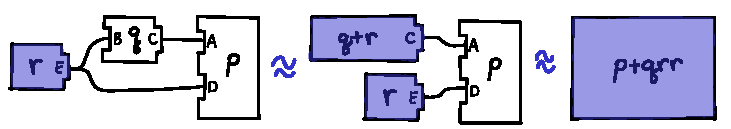
\includegraphics{figures/unit-identifier-improvement.pdf}
\end{figure}

\section{Modifications to GHC}

As far as possible, the typechecking rules described in
\cref{sec:compiler} are a faithful rendering of our
actual implementation of \Backpack{} in GHC\@: each rule
is in direct correspondence to some functionality in
GHC\@.  To help readers interested in perusing \Backpack{} in GHC's
source code, \cref{table:semantic-objs} gives a correspondence
between a semantic object and its corresponding type name in GHC\@;
similarly, \cref{table:judgments} gives a correspondence between
our judgments and their implementations in GHC\@.

In our primary \Backpack{} patch (not counting subsequent bugfix
patches, as well as some preliminary support for signatures that we had
committed previously), we modified 40 files in the compiler (out of 513
source files in the \verb|compiler| directory), adding 4375 lines and
deleting 588 lines.  In this respect, we think that our \Backpack{}
patch is quite well-contained: by and large, we were able to implement
\Backpack{} with minimal changes to the renamer and typechecker.
However, there is one major complication, related to GHC's lack
of \emph{symbol tables}, which we discuss in the next section.

\begin{table}
\centering
\begin{tabular}{llllll}
Semantic entity & & GHC type & Defined In \\
\midrule
Module name & $m$ & \verb|ModuleName| & \verb|Module| \\
Component identifier & $p$ & \verb|ComponentId| & \verb|Module| \\
Module identifier & $M$ & \verb|Module| & \verb|Module| \\
Unit identifier & $P$ & \verb|UnitId| & \verb|Module| \\
Module type & $T$ & \verb|ModIface|/\verb|ModDetails| & \verb|HscTypes| \\
Type declaration & \I{decl} & \verb|IfaceDecl|/\verb|TyThing| & \verb|IfaceSyn|/\verb|TyCoRep| \\
Class instance & \I{inst} & \verb|IfaceClsInst|/\verb|ClsInst| & \verb|IfaceSyn|/\verb|InstEnv| \\
Family instance & \I{inst} & \verb|IfaceFamInst|/\verb|FamInst| & \verb|IfaceSyn|/\verb|FamInstEnv| \\
Occurrence name & $n$ & \verb|OccName| & \verb|OccName| \\
Original name & $N$ & \verb|Name| & \verb|Name| \\
Name substitution & $\USn$ & \verb|NameShape| & \verb|NameShape| \\
Haskell type/kind & $\tau, \kappa$ & \verb|IfaceType|/\verb|Type| & \verb|IfaceType|/\verb|TyCoRep| \\
External component type context & $\Gamma$ & \verb|ExternalPackageState| & \verb|HscTypes| \\
Local type context & $\Delta$ & \verb|HomePackageTable| & \verb|HscTypes| \\
\end{tabular}
\caption{Mapping from semantic objects in this thesis (\cref{fig:lcomponents} and \cref{fig:semantic-objects}) to their definitions
in GHC\@.  In some cases, a semantic object maps to two types in GHC\@; see \cref{sec:no-symbol-tables} for details.}
\label{table:semantic-objs}
\end{table}

\begin{table}
\centering
\begin{tabular}{llll}
Figure & Judgment & GHC Function & Defined In \\
\midrule

\Cref{typing:haskell} & Module/signature typechecking & \verb|tcRnModule| & \verb|TcRnDriver| \\
& Type/kind equality & \verb|eqType| & \verb|Type| \\
& Instance resolution & \verb|check_inst| & \verb|TcBackpack| \\

\Cref{typing:main} & Top-level typing & \verb|load| & \verb|GhcMake| \\
& \quad\textsf{exposes} & \verb|applyPackageFlag| & \verb|Packages| \\
& \quad\textsf{inherits} & \verb|collectHoles| & \verb|Packages| \\
& Declaration typing & \verb|hscTypecheck| & \verb|HscMain| \\
& Dependency typing & \verb|tcRnCheckUnitId| & \verb|TcBackpack| \\
& Declaration sequencing & \verb|upsweep| & \verb|GhcMake| \\

\Cref{typing:lookup} & Original name type lookup & \verb|importDecl| & \verb|LoadIface| \\
& Module type lookup & \verb|loadInterface| & \verb|LoadIface| \\
& Substitution & \verb|rnModIface| & \verb|RnModIface| \\
& Name substitution & \verb|rnIfaceGlobal| & \verb|RnModIface| \\
%& Orphan substitution & (implicit) & \\

\Cref{typing:merging} & Signature type merging & \verb|tcRnMergeSignatures| & \verb|TcBackpack| \\
& Export list merging & \verb|extendNameShape| & \verb|NameShape| \\
& Declaration list merging & \verb|mergeIfaceDecls| & \verb|TcIface| \\

\Cref{typing:top-subtyping} & Module subtyping & \verb|checkImplements| & \verb|TcBackpack| \\

\Cref{typing:subtyping} & Declaration subtyping & \verb|checkBootDecl| & \verb|TcRnDriver| \\
& Declaration pre-subtyping & \verb|checkBootTyCon| & \verb|TcRnDriver| \\
\end{tabular}
\caption{Mapping from typing judgments to implementations in GHC.}
\label{table:judgments}
\end{table}


\subsection{No symbol tables}
\label{sec:no-symbol-tables}

The most important aspect of the implementation not captured by
the rules in \cref{sec:compiler} is GHC's lack of traditional
symbol tables.
Traditionally, compilers have one or more data structures known as
\emph{symbol tables}, which are mappings from symbols to information
about the symbol: abstractly, the symbol table is represented by
the \emph{context} in which typechecking takes place.
Rather than look up information on symbols in a
context, GHC records all of the information about a symbol in
the symbol itself, forming an immutable cyclic data structure of
all symbols known to GHC\@.

For example, here are
some data types for the graph representation from GHC (simplified
and abbreviated):

\begin{lstlisting}
    data Type  = TyConApp TyCon [Type]  | ...
    data TyCon = SynonymTyCon Name Type | ...
    data ModDetails = ModDetails [TyCon] ...
\end{lstlisting}
%
A type may be an application of a type constructor to some arguments, in which
case it contains a type constructor \verb|TyCon|.  A type constructor
can be a type synonym, in which case it contains the type it expands
to.  A module \verb|ModDetails| consists of a list of type constructors
and other entities that are defined in it.  The ``graph'' is the graph of
heap objects which represent these data types.

This graph is very convenient to work with in a purely functional
language like Haskell, since queries can be answered by a direct field
access rather than a lookup in a symbol table.  For example, type
equality can be defined as a pure function \verb|Type -> Type -> Bool|
even in the presence of type synonyms, since the \verb|SynonymTyCon|
always carries along the expanded version of the synonym to compare
against.

On disk, GHC must serialize these direct references to indirect references
by names:

\begin{lstlisting}
    data IfaceType = IfaceTyConApp Name [IfaceType] | ...
    data IfaceDecl = IfaceSynonym OccName IfaceType | ...
    data ModIface = ModIface [IfaceDecl] ...
\end{lstlisting}

\noindent
Unlike the graph representation, the type constructor application
doesn't embed the definition of the type constructor---instead,
it records only a \verb|Name| reference to the constructor. To find out
more information about the type constructor, you would have to lookup
the \verb|IfaceDecl| from the appropriate symbol table; e.g., a module
local declaration would be found in the \verb|IfaceDecl| list in
\verb|ModIface|.

GHC uses a technique called tying the knot
to construct the graph representation from the interface
representation: any time we encounter a \verb|Name|, GHC instead
allocates a thunk to lookup the appropriate declaration later,
once all of the entities have been added to the environment;
this is referred to as ``typechecking'' the interface.

\paragraph{Consequences for \Backpack{}}
In \cref{sec:overview-compiler}, we informally described
types as graphs, with original names pointing to the corresponding
declaration.  In fact, this is an accurate representation of how
these operations are implemented in GHC\@!

One downside of the immutable graph representation is that it is
difficult to modify after the fact: in general, the only way to update
it is to rebuild the graph from scratch.  Modifications of this kind
frequently occur in \Backpack{}: for example, applying a name
substitution will change how the graph is wired.

To handle this, our implementation does most operations in two
phases:

\begin{itemize}
    \item We first perform any operations which would
    mutate the graph on the \emph{interface representation}.
    These operations includes both module and name substitutions, as well
    as signature merging.
    \item Then, we generate the \emph{graph representation} from
    the resulting interface representation, and then perform any
    operations which require consulting the context.  These
    operations include subtyping, which test equality on types
    and require the context.
\end{itemize}
%
Module type lookup is a good example of this two phase process: to
perform module type lookup, we first read in the un-substituted
\verb|ModIface| from the file system, apply the substitution according
to the substitution in the module identity, and \emph{then} typecheck
the interface into the graph representation for using during type
checking.

A more subtle example of this process occurs when performing
signature merging.  When we merge signatures, we eventually need
to check that the merged signature is a subtype of each of the
input signatures, with the \emph{merged} signature in the context.
This means that to perform this subtyping test, GHC first typechecks
each of the input \verb|ModIface|s for the signatures, wiring any
local \verb|Name|s to point to the merged signature, and then performs
the subtyping tests on the resulting graph.  In other words, the
informal description of signature merging in \cref{sec:signature-merging}
is actually quite close to what actually occurs in GHC proper!

\subsection{Miscellaneous differences}

There are a number of smaller differences between our formalization
and GHC's representation.

\begin{itemize}
    \item In our formulation of GHC Haskell's semantic objects, an
    instance directly records the type representing the constraint that
    the instance fills.  In GHC Haskell, an instance instead contains a
    reference to a \emph{dictionary function}, which is just a type of
    term declaration that is never exported.  The two presentations are
    equivalent, but embedding the dictionary function in the instance
    makes it easier to specify the rules for instance checking (indeed,
    refactoring GHC to adopt this representation would substantially
    simplify some aspects of the implementation).  Similarly,
    closed family instances are associated with a coercion axiom, but in
    our presentation they are embedded in \I{tfinfo}; because coercion axioms
    are always associated with another declaration, we omit them from the
    production $\Uty$.

    \item We simplified export specifications to just be a list of
    names, rather than names with children (which allows GHC to support
    import declarations like \verb|import Prelude (Eq(..))|).  We've
    implemented an extension to handle children as per Haskell'98; the
    tricky thing is handling the semantics of an export of a bare
    record selector (without the type it is bundled with):

    \begin{lstlisting}
        module A where
            data T = MkT { f :: Int }
        module B(f) where
            import A
        module C(T(..)) where
            import A (T)
            import B (f)
    \end{lstlisting}

    Haskell'98 specifies that \verb|T(..)| selects both \verb|T| and \verb|f|
    for export: a record selector always ``remembers'' what type is its
    parent.  In Haskell'98, a record selector or data constructor
    always comes from the same module as the parent, so when
    we apply a name substitution to \verb|f|, we can infer the new name of
    the parent with directly from the substituted name.

    There are two more features in GHC Haskell which affect export lists:
    \begin{itemize}

        \item Bundled pattern synonyms\footnote{\url{https://ghc.haskell.org/trac/ghc/wiki/PatternSynonyms/AssociatingSynonyms}} make it possible to declare a pattern synonym
            to be a child of a type: in this case, the child of a type may
            be defined in a different module than the type itself.
            \Backpack{} does not support pattern synonyms, so it's
            not possible to have nontrivial bundling between an abstract
            pattern synonym or abstract type in a signature file, but if it
            were to support pattern synonyms this interaction would need to
            be worked out.

        \item Duplicate record fields\footnote{\url{https://ghc.haskell.org/trac/ghc/wiki/Records/OverloadedRecordFields/DuplicateRecordFields}} augment
            every export with a set of associated ``field labels'', which are
            allowed to overlap with other field labels that are in scope.
            These are handled similarly to exported children.
        \end{itemize}

    \item In our formalization, the list of transitive orphan-defining
        modules includes the module itself; GHC stores this separately
        in another flag in the interface file.

    \item In the abstract grammar for module identifiers ($M$) and original
        names ($N$), we have separate cases for module holes and name
        holes.  In GHC, we avoid defining an extra constructor
        by instead defining a special unit identifier \cidl{hole}, and saying
        that a module hole $\hv{m}$ is represented as \Mod{\cidl{hole}}{m};
        similarly, a name hole  \nhv{m.n} is represented as $\Mod{\cidl{hole}}{m}.n$.

        Internally representing the holes this way was expedient as it
        allowed us to avoid having to add a lot of new pattern matches
        to GHC, but the tradeoff is that we have to be careful about how
        we go about performing substitutions.  If I have
        $\Mod{\cidl{hole}}{m}.n$ (i.e., $\nhv{m.n}$) and apply the
        substitution $m = M$ to it, I better not end up with $M.n$.

        For example, we must not apply
        a module substitution on the module identifier of an original name,
        if its top level module identity is a hole module.

    \item Modifications to GHC's \verb|UnitId| data type to support module
        substitutions.  We try to keep \uid{}s represented as plain
        strings as much as possible; see \cref{sec:opaque-uid} for
        more details.

    \item We applied a slight optimization when testing that an instantiated
        dependency is well-typed:
        rather than defer this type checking to the
        very end of compilation, we incrementally check dependencies for well-typedness
        as we finish typechecking all the local signatures for the dependency's
        requirements.

    \item Modules declared in \verb|other-modules| cannot be reexported,
        as \verb|ghc-pkg| verifies that a module is truly exposed
        (\verb|other-modules| are truly implementation details of the
        packages in question.)

\end{itemize}
%


\section{Modifications to Cabal}

Our implementation of \Backpack{} in Cabal also closely follows the description
from \cref{sec:overview}.  There are three primary phases in our
implementation:

\begin{enumerate}
    \item Given the original Cabal source file, we elaborate each
    component it defines into \emph{configured component},
    for which we've resolved all source-level dependencies
    (e.g., entries in \verb|build-depends|) to the specific
    \cid{}s representing them, incorporating in the information
    we learned from dependency resolution.

    \item We then perform mixin linking, producing \emph{linked component}
    where every \cid{} has been further elaborated into a \uid{}
    representing exactly how the dependencies are instantiated.
    Mixin linking is essentially a direct implementation of the
    description we gave in \cref{sec:mix-in}.

    \item Finally, we zip through all fully instantiated components
    and recursively instantiate their dependencies, producing one or
    more \emph{ready components} per source component.  Each ready
    component represents a component plus a complete instantiation,
    and represents a separate compilation we will do (with full
    knowledge of how the dependencies are instantiated).
\end{enumerate}
%
We did need to apply one nontrivial architectural change to Cabal.
Previously, Cabal was organized into two parts:

\begin{itemize}
    \item The \emph{build system}, e.g., Cabal, which is responsible for
    building a single package, and

    \item The \emph{package manager}, e.g., cabal-install, which is
    responsible for building multiple packages.
\end{itemize}
%
A single package may itself contain multiple components (beyond the library,
there may be test suites, executables, etc.). Historically, a package manager
invoked Cabal the build system once to build all the components at once.

This architecture causes problems for \Backpack, where a library may need
to be built multiple times because it was reinstantiated: in this case, we really want to
rebuild just the library (and not the executables, test suites, etc.).
So, instead, we added a new mode to the Cabal build system to operate
on a per-component basis:\footnote{https://github.com/ghc-proposals/ghc-proposals/pull/4}
the \emph{build system} builds a single \emph{component}, and
the \emph{package manager} builds multiple components.  For \Backpack{} to be
supported by Stack (an alternative package manager implementation), we'll have
to apply this architectural change as well.

%!TEX root = paper.tex

\chapter{Evaluation}
\label{sec:evaluation}

% Audience:
%   - Does Backpack work?
%   - Does it solve my problems?
%   - Should I use it?
%   - Is the extension maintainable?

How can we tell if \Backpack{} works?  The proof of the pudding is
in the eating: in this chapter, we describe some of the case studies
we've implemented using \Backpack{} to help validate our implementation.

\section{Parametrizing a library}

A number of well-known packages in the Haskell ecosystem are parametric over
implementations of certain core types.  To show \Backpack{} is sufficient
to handle real world examples, we used \Backpack{} to
reparametrize \verb|unix|, \verb|tagstream-conduit| and \verb|reflex| packages, replacing
the previous strategies these packages used to support multiple
implementations of core types.  We've chosen to showcase these three
packages as they ended up being Backpack'ed in quite different ways.

\subsection{Removing copy-pasted code from unix}

The \texttt{unix}\footnote{\smaller\url{https://github.com/haskell/unix}} package provides both \verb|String| and
\verb|ByteString| versions of modules by having multiple copies of the
module with slight modifications.  For example,  here are the \verb|String|
and \verb|ByteString| versions of the \verb|getEnv| function:

\begin{lstlisting}
    -- System.Posix.Env
    getEnv :: String -> IO (Maybe String)
    getEnv name = do
        litstring <- withFilePath name c_getenv
        if litstring /= nullPtr
            then liftM Just (peekFilePath litstring)
            else return Nothing
\end{lstlisting}

\begin{lstlisting}
    -- System.Posix.Env.ByteString
    getEnv :: ByteString -> IO (Maybe ByteString)
    getEnv name = do
        litstring <- B.useAsCString name c_getenv
        if litstring /= nullPtr
            then liftM Just (B.packCString litstring)
            else return Nothing
\end{lstlisting}
%
The structure of the code between for these modules is essentially identical,
except for a few identifiers: \verb|String| versus \verb|ByteString|,
\verb|withFilePath| versus \verb|B.useAsCString|, and \verb|peekFilePath|
versus \verb|B.packCString|.

To convert this function to use \Backpack{}, we created
a signature file which covers the identifiers which vary across the
two implementations:

\begin{lstlisting}
    signature Str where
        import Foreign.C.String (CString)
        data Str
        useAsOSString :: Str -> (CString -> IO a) -> IO a
        packOSString :: CString -> IO Str
        -- ... and more for other functionality
\end{lstlisting}
%
\ldots{}and then rewrote the modules to import the signatures and use
them instead:

\begin{lstlisting}
    import Str
    getEnv :: Str -> IO (Maybe Str)
    getEnv name = do
        litstring <- withOSString name c_getenv
        if litstring /= nullPtr
            then liftM Just (packOSString litstring)
            else return Nothing
\end{lstlisting}
%
There were five modules for which there were both \verb|String| and
\verb|ByteString| variants. We divided these modules into three packages based
on what functionality they needed:  \verb|unix-env| required \verb|Str|,
\verb|unix-fs| required \verb|FilePath|, and \verb|unix-process|, which
required both \verb|Str| and \verb|FilePath|.  We also added a new
package \verb|unix-common| to store functionality that did not depend
on strings or filepaths specifically.

Consequently, we were able to delete the five duplicates of these
modules---removing 954 lines of code including comments and white space.
The total savings are a bit less, because we added source code for the
signatures, implementations of the signatures and new Cabal files for
each of the new packages.  However, the signatures and implementations
can be reused over multiple packages, and the resulting packages are
\emph{more} flexible, in the sense that they can be instantiated with
any string implementation an end user wants.

\subsection{Removing dictionary-passing style from tagstream-conduit}

The \texttt{tagstream-conduit}
package\footnote{\smaller\url{https://hackage.haskell.org/package/tagstream-conduit}}
is an HTML tag parser that supports both \verb|Text| and
\verb|ByteString|, using a record of functions to parametrize over key
string manipulation functions.  For example, here is the implementation
of \verb|decodeEntitiesText|, which operates on the \verb|Text| type:

\begin{lstlisting}
-- | Decode the HTML entities e.g. @&amp;@ in some text into @&@.
decodeEntitiesText :: Monad m => Conduit Token m Token
decodeEntitiesText =
  decodeEntities
    Dec { decToS     = L.toStrict . B.toLazyText
        , decBreak   = T.break
        , decBuilder = B.fromText
        , decDrop    = T.drop
        , decEntity  = decodeEntity
        , decUncons  = T.uncons }
  where decodeEntity entity =
          CL.sourceList ["&",entity,";"]
          $= XML.parseText def { XML.psDecodeEntities = XML.decodeHtmlEntities }
          $= CL.map snd
          $$ XML.content
\end{lstlisting}
%
\verb|decodeEntities| is a parametric function which takes the
\verb|Dec| structure as an argument.  Its type signature is:

\begin{lstlisting}
    decodeEntities :: (Monad m, Monoid builder, Monoid string,
                       IsString string, Eq string)
                   => Dec builder string
                   -> Conduit (Token' string) m (Token' string)
\end{lstlisting}
%
\verb|Dec| in turn is a structure
that contains implementations for each of the operations:

\begin{lstlisting}
    -- | A decoder.
    data Dec builder string = Dec
      { decToS     :: builder -> string
      , decBreak   :: (Char -> Bool) -> string -> (string,string)
      , decBuilder :: string -> builder
      , decDrop    :: Int -> string -> string
      , decEntity  :: string -> Maybe string
      , decUncons  :: string -> Maybe (Char,string)
      }
\end{lstlisting}
%
In \Backpack{}, we monomorphized \verb|decodeEntities|, replacing
it with an implementation that utilized signatures for strings:

\begin{lstlisting}
    signature Str where
        import Data.String

        data Str

        instance Monoid Str
        instance IsString Str
        instance Eq Str

        drop         :: Int -> Str -> Str
        decodeEntity :: Str -> Maybe Str
        uncons       :: Str -> Maybe (Char, Str)
        break        :: (Char -> Bool) -> Str -> (Str, Str)
\end{lstlisting}
%
\ldots{}and string builders:

\begin{lstlisting}
    signature Builder where
        import Str

        data Builder
        instance Monoid Builder

        builderToStr :: Builder -> Str
        strToBuilder :: Str -> Builder
\end{lstlisting}
%
Additionally, the \verb|Text| and \verb|ByteString|
modules also had some copy-pasted code for miscellaneous parsing
functionality; we extended the string signature with seven more
functions and added a signature for parsers:

\begin{lstlisting}
    signature Parser where

    import Control.Applicative
    import Str

    data Parser a
    instance Functor Parser
    instance Applicative Parser
    instance Monad Parser
    instance Alternative Parser

    anyChar :: Parser Char
    takeTill :: (Char -> Bool) -> Parser Str
    char :: Char -> Parser Char
    satisfy :: (Char -> Bool) -> Parser Char
    string :: Str -> Parser Str
    skipSpace :: Parser ()
    takeRest :: Parser Str
    parseOnly :: Parser a -> Str -> Either String a
\end{lstlisting}
%
With this refactor, we removed 258 lines of duplicated implementation
code and also eliminated the indirection in the implementation
of \verb|decodeEntities|, making it possible for GHC to inline
these functions---in the old version of the code, this would only
be possible if \verb|decodeEntities| was inlined at its call-sites
in \verb|decodeEntitiesText| and \verb|decodeEntitiesBS|.  (GHC
may not do this if \verb|decodeEntities| is a large function.)

\subsection{Removing type class indirection from Reflex}

Reflex is a framework for high-performance functional reactive
programming.  It has two implementations of its core ``timeline'' (the core
engine responsible for scheduling and dispatching events):
a pure but inefficient reference implementation, and a fast
Spider timeline based on mutable state.  Most real world users
will only make use of the Spider timeline, but the test suite
uses the reference implementation to check the correctness of the
more complicated Spider timeline.

Ordinarily, these implementations are abstracted over the \verb|Reflex|
type class:

\begin{lstlisting}
    class ( MonadHold t (PushM t)
          , MonadSample t (PullM t)
          , MonadFix (PushM t)
          , Functor (Dynamic t)
          , Applicative (Dynamic t)
          , Monad (Dynamic t)
          ) => Reflex t where
      data Behavior t :: * -> *
      data Event t :: * -> *
      data Dynamic t :: * -> *
      data Incremental t :: * -> *
      type PushM t :: * -> *
      type PullM t :: * -> *
      pull :: PullM t a -> Behavior t a
      -- 19 more methods
\end{lstlisting}
%
Compiled na\"\i{}vely, code that makes use of this type class know nothing
about the underlying implementation of these methods, thwarting GHC's
inliner and optimizer. This is a big loss, since most of the time you
only needed the Spider timeline implementation.  In fact, even when
the implementation is statically known via the type a method is used
at, GHC will still occasionally fail to specialize\footnote{\url{https://ghc.haskell.org/trac/ghc/ticket/12791}
and \url{https://mail.haskell.org/pipermail/ghc-devs/2016-October/013170.html}},
causing a huge slowdown.

With Reflex, we investigated using \Backpack{} to eliminate all uses of
the \verb|Reflex| type class, thus eliminating dictionaries altogether.
Backpack'ing Reflex posed some unique problems:

\begin{itemize}
    \item The Spider timeline's type is not \verb|SpiderTimeline|
        but \verb|SpiderTimeline x|---in particular, it takes a phantom
        type parameter similar to the \verb|s| of the \verb|ST|
        monad~\cite{Launchbury:1994:LFS:773473.178246} that is used to
        distinguish between different running instances of the Spider
        timeline.

        This is not a problem for the \verb|Reflex| type class:
        if we declare an instance of \verb|Reflex| for \verb|SpiderTimeline x|
        we get the following type signature for the method \verb|pull|:

        \begin{lstlisting}
        pull :: PullM (SpiderTimeline x) a -> Behavior (SpiderTimeline x) a\end{lstlisting}
        Here, the signature states that if we call pull on a \verb|PullM|
        from a Spider timeline, we will get a \verb|Behavior|
        from the very same Spider timeline.

        However, if in \Backpack{} we existentially quantify
        the type variable \verb|x| to create a well formed
        top-level type declaration, we will end up with the
        following types:

        \begin{lstlisting}
        data Timeline = forall x. SpiderTimeline x
        pull :: PullM Timeline a -> Behavior Timeline a\end{lstlisting}
        This doesn't have the intended semantics: here, \verb|pull|
        accepts a \verb|PullM| from some timeline, and then gives
        you a \verb|Behavior| from another timeline, but doesn't tell
        you if they are the same or not, making it impossible to tell
        statically if you are mixing up two different timelines or not.

    \item Unlike the previous two case studies, we wanted to build
        the \Backpack{} interfaces on top of the existing Reflex
        library without modifying it at all, so that clients could
        choose between the old-style type-class based interface, or
        the new-style \Backpack{} interface.  This meant, as much
        as possible, we wanted to reuse types and classes from
        Reflex, as long as they did not depend on the \verb|Reflex|
        type class.  (We can't reuse declarations which depend
        on \verb|Reflex|, since our intention is to specialize the
        type class away.)

%   \item Reflex defines a large number of type classes which mention
%       the associated types of \verb|Reflex|.  These type classes
%       cannot be easily eliminated via \Backpack{} (classes like
%       \verb|MonadHold| and \verb|MonadSample| are for allowing
%       users to use functions on arbitrary monad transformer stacks),
%       but must be defined
\end{itemize}
%
Here is an excerpt for the signature we wrote for Reflex:

\begin{lstlisting}
    data Timeline t
    class HasTimeline t

    type Event          t = C.Event         (Timeline t)
    type Dynamic        t = C.Dynamic       (Timeline t)
    type Behavior       t = C.Behavior      (Timeline t)
    type Incremental    t = C.Incremental   (Timeline t)
    type EventSelector  t = C.EventSelector (Timeline t)

    data PushM t a
    data PullM t a

    instance HasTimeline t => MonadHold     (Timeline t) (PushM t)
    instance HasTimeline t => MonadSample   (Timeline t) (PullM t)
    instance HasTimeline t => MonadFix      (PushM t)
    instance HasTimeline t => Functor       (Dynamic t)
    instance HasTimeline t => Applicative   (Dynamic t)
    instance HasTimeline t => Monad         (Dynamic t)
    -- Instances for the superclasses

    pull :: HasTimeline t => PullM t a -> Behavior t a
\end{lstlisting}
%
There are a number of things to point out about this signature:

\begin{itemize}
    \item The abstract type representing timelines is
        \verb|data Timeline t|, taking a phantom type parameter
        which will be used to track timelines.
        Reflex also associates this phantom type parameter with
        a class constraint \verb|HasSpiderTimeline|, so we need
        an abstract class \verb|HasTimeline| to abstract over
        this extra constraint (we can implement this class using
        a constraint synonym).

    \item Rather than define abstract types for \verb|Event|,
        \verb|Dynamic| and the other associated data families,
        we instead require them to be type synonyms of the
        appropriate data family for our abstract type \verb|Timeline|.
        The benefit of doing things this way is that we can
        reuse the existing \verb|MonadHold| and \verb|MonadSample|
        type classes which don't use the \verb|Reflex|
        type class directly, but do refer to the associated
        data families it defines.

        In contrast, the type synonym families get abstract
        types, because we need to declare instances on them,
        and Haskell unconditionally forbids type family applications in
        instances.\footnote{GHC Haskell should relax its rule
        to forbid type family applications which contain free
        variables, which would be sufficient to avoid undecidability
        of instance resolution.  See also
        \url{https://ghc.haskell.org/trac/ghc/ticket/13262}}

    \item In a signature, a user is required to declare
        instances not only for any classes they want to support,
        but also all of the superclasses of those classes.  For
        brevity, we've
        omitted those superclasses.

    \item Inside the module parametrized over this signature,
        we defined some instances which overlapped with existing
        instances from the Reflex library.  For example, Reflex
        defines an instance \verb|instance Reflex t => Behavior t|,
        which makes use of the \verb|Reflex| type class to provide
        operations,
        while we define \verb|instance Behavior (Timeline t)|, which
        directly makes use of operations from the signature.
        Fortunately, the second specialized instance is more specific
        than the first instance, so it is preferred during instance
        resolution.
\end{itemize}
%
Reflex also has a separate interface, \verb|ReflexHost|, for listening
to events, which is only supported by the Spider implementation.
To accommodate this, we created another library which mixed in
the basic Reflex functionality and extended the signature with the
extra requirements that were needed.

\section{Replacing build-depends with signatures}

One of the future applications we envision for \Backpack{} is subsuming
traditional version bounds in packages.  To show that \Backpack{} is up
to the task, we took a few packages in the public Hackage repository and
rewrote them to deprecate some of their \verb|build-depends| in favor of
signatures instead:

\begin{itemize}
    \item We rewrote \texttt{binary-0.8.0.0}\footnote{\smaller\url{https://hackage.haskell.org/package/binary-0.8.0.0}}
          to have signatures
          for \texttt{byte\-string}, \texttt{containers} and \texttt{array},
          demonstrating that GHC's core libraries can be modularized
          over. (23 signatures)

    \item We rewrote \texttt{ghc-simple-0.3}\footnote{\smaller\url{https://hackage.haskell.org/package/ghc-simple-0.3}} to have signatures
          for \texttt{ghc}, demonstrating that the GHC API (a very
          complicated API) can be modularized over. (57 signatures)
\end{itemize}
%
For example, here is the signature we wrote for
\texttt{Data.\allowbreak{}Array.\allowbreak{}IArray} in \texttt{binary},
exercising many of Haskell's features including type classes:

\begin{verbatim}
    {-# LANGUAGE RoleAnnotations #-}
    {-# LANGUAGE FlexibleInstances #-}
    {-# LANGUAGE MultiParamTypeClasses #-}
    {-# LANGUAGE KindSignatures #-}
    {-# LANGUAGE ExplicitForAll #-}
    module Data.Array.IArray (
        module Data.Array.IArray,
        module Data.Ix
        ) where

    import Data.Ix

    type role Array nominal representational
    data Array i e
    class IArray (a :: * -> * -> *) e
    instance IArray Array e
    bounds :: (IArray a e) => forall i. Ix i => a i e -> (i, i)
\end{verbatim}
%
Adding signatures to packages is a straightforward (if a little tedious)
process.  However, we made two interesting observations.

First, there is a certain amount of human judgment that needs to be
exercised when writing these signatures, because of the convention in
Haskell where a type may be defined in an ``internal'' module, and then
reexported by a more public module.  Consider these two situations:

\begin{itemize}
    \item The \verb|Map| type is publicly exported by \verb|Data.Map|
    but originally defined in \verb|Data.Map.Internal|.

    \item The strict \verb|ByteString| type is publicly exported by
    \verb|Data.ByteString| but originally defined in
    \verb|Data.ByteString.Internal|.
\end{itemize}
%
We ended up placing \verb|Map| in \verb|Data.Map|,
but \verb|ByteString| in \verb|Data.ByteString.Internal|, as
\verb|binary| used both \verb|Data.ByteString| and \verb|Data.ByteString.Internal|
to manipulate \verb|ByteString|s (we can't define the type in both locations,
since then they won't be the same type!).  In other cases, if a type is exported by
many modules, it may make sense to refactor the imports of the modules
so that we may declare it in a single signature.

Second, the lack of
\emph{recursively dependent signatures}~\cite{crary+:recmod-pldi}
(\ie, signatures that form an import cycle)
sometimes caused problems when a
dependency was implemented using \texttt{hs-boot} files to implement
recursion.  However, this could be easily worked around by adding
a ``synthetic'' signature which collected all of the mutually dependent
data types together, and then have the real signatures reexport
from this signature;  the synthetic signature is then implemented using
a dummy module.  Here is an example of such a synthetic signature
from \texttt{ghc-simple}'s signatures for GHC\@:

\begin{verbatim}
    module RecTypes where

    import ConLike  (ConLike)
    import CoAxiom  (Branched, CoAxiom)
    import OccName  (OccName)

    data Id      -- from Id,   imports Name
    data Name    -- from Name, imports Type
    data TyCon   -- from Type
    data TyThing -- from Type, imports Id
        = AnId Id
        | AConLike ConLike
        | ATyCon TyCon
        | ACoAxiom (CoAxiom Branched)
\end{verbatim}
Without this synthetic signature, the signatures for \texttt{Id}, \texttt{Name},
and \texttt{Type} would form a cycle.

We also have a negative result to report: we were unable to parametrize
the \verb|array| package over \verb|base|.  The difficulty is that
many language features are implemented by selecting a \emph{specific}
implementation from \verb|base|, bypassing the import mechanism.
This means that it's not possible to overload their
implementation merely by changing what module names are in scope.  This
affected a number of things:

\begin{itemize}
    \item Deriving type class instances,
    \item Rebindable syntax (e.g., do notation, integer literals
          and string literals),
    \item Foreign call marshalling, and
    \item Built-in types (e.g., \verb|Integer| for \verb|[0..n]|
          syntax, and booleans for pattern guards).
\end{itemize}
%
As \verb|base| is quite a large package, we think it would be beneficial
if users could write signatures for it; probably the most practical
way forward is to refactor \verb|base| into two packages, one that
contains wired-in entities, and one that does not.

%   \section{A signature for strings}

%   One of the motivating applications of \Backpack{} is handling the
%   so-called ``string problem'', where the Haskell ecosystem has
%   many implementations of string-like data types, and it is difficult
%   to write code that is parametric over the implementation of strings.
%   Indeed, both of the example parametrizations from the previous section
%   are dealing with strings of one form or another.

%   While a package can write a signature for all the functions on strings they
%   require from scratch, it is also useful to be able to reuse signatures
%   between packages.  To this effect, I created a string signature which
%   represented the union of the APIs provided for:

%   \begin{itemize}
%       \item \verb|String| from \verb|base|,
%       \item Strict/lazy ASCII/binary \verb|ByteString| from \verb|bytestring|,
%       \item Strict/lazy UTF-8 \verb|ByteString| from \verb|utf8-string|,
%       \item Strict/lazy \verb|Text| from \verb|text|, and
%       \item \verb|String| from \verb|foundation|
%   \end{itemize}

%   \Red{finish this section}

\section{An alternate package language}
\label{sec:alternative-package-language}

A benefit of having a separation between mixin linking and typechecking
is that it is a simple matter to swap the frontend language with
something else.  To assist in testing Backpack, we implemented a simple
alternate frontend that operates on mixed components (i.e.\ post mixin
linking):

\begin{verbatim}
    unit p where
        dependency base
        signature H where
            data T
        module M where
            import H
    unit q where
        dependency p[H=<H>]
        module N where
            import M
\end{verbatim}
%
The above source code can be run using the \verb|--backpack| major mode
in GHC\@.  This frontend language is used extensively in our test suite
(of over a hundred test cases): in particular, the inline module and
signature syntax is extremely convenient.  This format is not intended
for real world use, since it is difficult to get accurate recompilation
avoidance when source code is all in one file.

\chapter{Limitations and future directions}
\label{sec:limitations}

\section{Metatheory}
\label{sec:metatheory}

We have not rigorously done proofs on \Backpack{}'s metatheory; as such,
we can only conjecture that in the fragment of Haskell \emph{without type
classes and type families}, successful separate typechecking of
components implies successful linking as well.  Conventionally,
soundness proofs for module systems are done by elaboration to an
appropriate internal language; however, it is difficult to say what an
internal language which supports all of GHC Haskell's features would
look like, and in any case, a proof about this elaboration would say
little about the actual typechecking algorithm that GHC
implements.  \OldBackpack{}'s proof
of soundness gives evidence that \Backpack{} is sound, but we leave
an actual formalization to future work.

Note that the soundness of \emph{compiled} \Backpack{} code reduces to
the soundness of GHC Haskell, because we retypecheck and compile every
instantiation of a component. Thus, at the end of the day, compilation
of \Backpack{} code reduces to ordinary Haskell
compilation.\footnote{This is similar to the situation with Java
generics, where erasure at the JVM level means that an unsound type
checking algorithm for generics will only result in an invalid cast
exception at runtime; unlike Java, any errors in \Backpack{} are caught
at instantiation-time.}  However, one should still ask tough questions
about the soundness of recursive modules, which is a feature in its own
right; and indeed, there is at least one known bug where \verb|hs-boot|
files can cause
unsoundness.\footnote{\url{https://ghc.haskell.org/trac/ghc/ticket/9562}}

\subsection{Type classes and type families}

Note that we stated that \Backpack{} is sound \emph{without} type classes
and type families.  The soundness result we desire is not true for full
Haskell, and in fact, it cannot be made to be true as Haskell exists today.
Ordinary proofs of soundness rely on weakening: the ability of a signature
to hide information about its implementation.
Open type families~\cite{schrijvers+:typefamilies}
introduce axioms to Haskell which cannot be hidden by signatures:

\begin{lstlisting}
    signature A where
        f :: F Bool

    module B where
        import A
        type instance F Bool = Int -> Bool
        x = f 2
\end{lstlisting}
%
Now, should the following module be a permissible implementation of the
signature?

\begin{lstlisting}
    module A where
        type instance F Bool = Int
        f :: F Bool
        f = 42
\end{lstlisting}
%
Comparing only the signature and the module, it might seem that, yes,
the module is a permissible implementation, as it provides all of the
declarations required in the signature.  But if we do allow it,
then \verb|B| is clearly type unsafe, attempting to use an integer
as a function.

Is this problem fixable?  One ``fix'' is to require signatures to
specify every type family instance that an implementation could possibly provide:
but it should be clear that such signatures would contain many ``irrelevant''
instances to the parametrization at hand.  Another fix is to change the rules for
permissible type family instances, so that instances defined in separate
modules are guaranteed not to conflict, no matter what.  But this would
constitute a fundamental change to how open type families work in
Haskell and rule out existing Haskell code.

So, why isn't the lack of modularity with respect to type classes a
total disaster for \Backpack{}?  Why won't Haskell programmers riot in
the streets when their programs typecheck separately, but fail to link
together?  Based on our experiences writing programs with
\Backpack{}, there are two reasons:

\begin{itemize}
    \item By in large, the Haskell ecosystem tries very hard to
    \emph{not} have conflicting instances in the modules we define,
    eschewing \emph{orphan instances} which are the primary mechanism
    by which conflicts can arise.\footnote{A non-orphan instance is one that
    is defined along side the type or class it corresponds to, and can
    be thought of as an ``intrinsic'' property of the type/class it was
    deifned with, making it difficult---though not impossible---to
    create a conflict.}
    Generally, instantiating a \Backpack{} package with a module will
    not result in an instance conflict, in the same way that adding an
    import to a module will not result in an instance conflict.

    \item Assuming that there are no conflicting instances (a \emph{big}
    assumption, but one that seems to be true in practice), the only thing
    that a parametrized package must do is ensure that it is indifferent
    to the addition of new instances (rather than assert that we can thin
    them out.)  In practice, these means following the same best practices
    which prevent conflicts from occurring---e.g., avoiding orphan
    instances:

\begin{lstlisting}
    signature A where
        data T
    module B where
        import A
        instance Show T where ... -- bad!
\end{lstlisting}
%
    This is not difficult to do!
\end{itemize}
%
Thus, while we cannot give \emph{technical} rules which ensure the modularity
of \Backpack{}, the \emph{social} rules of Haskell allow us to maintain
modularity and separate compilation.

One final word: there is an unrelated gotcha related to type refinement
and instance declarations:

\begin{lstlisting}
    signature A where
        data T
        data S
    module B where
        import A
        class K a
        instance K T
        instance K S
\end{lstlisting}
%
This could fail to typecheck if T and S refine to the same type.  Arguably,
GHC should be able to tell when an overlap could occur, but it does not today.
To fix the code, you can either newtype T and S, or hoist K out of the
parametrized package.

%   The upshot is that, without changing how open type families work, we
%   must allow for the possibility that linking can fail, even if the
%   components typechecked separately.

% Trouble: declaring a local QuickCheck instances


% First thrust:
%   - Define appropriate orphanhoodness check sufficient to
%     prevent conflicting instances from being defined
%   - Trouble:
%       signature A where
%       module M where
%           import A
%           f = show True
%     Then suppose that A is implemented with a module which has
%     incoherent instances for Show Bool.  Need to *eagerly*
%     report conflict. But now you're in the same situation
%     as applying the eagerness globally (effectively)
%   - Suppose that "somehow conflicts don't happen" (this is
%     the case for type families.)  You can still get in trouble
%     if instantiation causes incompatible universes to collide:
%       signature A where
%       module M where
%           import Inst1
%           -- ... use instance
%     if A is filled with something using (incompatible) Inst2,
%     once again we blow up when we instantiate

\section{Mutually recursive packages}

We have not described how to handle mutual recursion in \Backpack{},
although we believe that \Backpack{} can be extended to accommodate it,
based off of GHC's existing support for \verb|hs-boot| files.
Indeed, we showed in Section~\ref{sec:recursive-uids} that recursive
\uid{}s can be handled in the same way as they were done in \OldBackpack{}.

One challenge that we face is how to handle the ``double vision
problem'' in the presence of type synonyms.  \OldBackpack{} solved the
double vision problem for original names via  shaping pass; however,
languages like MixML which permit transparent type synonyms also have
required a type pre-computation pass to to solve double-vision at the
type level.

Interestingly, GHC's type checking algorithm is already designed in
such a way that it can solve the double vision problem in the following
way: an abstract type is opaque except within the \emph{implementing
module} (and any module which imports this module) at which point one
sees the value of the type synonym.

\begin{lstlisting}[language=Haskell]
    -- A.hs-boot
    module A where
        data T
        f :: T -> T
    -- B.hs
    module B(f) where
        import {-# SOURCE #-} A
    -- A.hs
    module A(T, f) where
        import qualified B
        type T = Int
        f :: Int -> Int
        f x = B.f x
\end{lstlisting}
%
When typechecking \verb|A.hs|, GHC resolves the type \verb|T| within
\verb|B.f| to be the type synonym \verb|type T = Int|, \emph{in the very
same module it is typechecking}.  In a sense, GHC has ``solved'' the
double vision problem, though it's worth noting that systems like RMC
and MixML address a stronger version of the double vision problem which
is inapplicable to Haskell due to the lack of sealing (see
Appendix~\ref{sec:double-vision}).  (In reality, GHC rejects \verb|A.hs|
because it does not allow abstract data to be implemented with type
synonyms, but in principle this restriction could be relaxed.)

\section{The signature language}

It is reasonably well understood how to reuse \emph{code}: functions and
values that need to be used multiple times are bundled into modules, and then
used by their downstream clients.  Less clear is how one goes about
reusing \emph{signatures}.

In \Backpack{}, we offer some limited facilities for signature reuse.
The most basic, essential form of signature reuse in a package language
based on mix-ins is \emph{signature merging}; this functionality is
essential for composing libraries with requirements, since without it,
we would have to manually rewrite the signature every time we put two
such libraries together.  In degenerate form, this allows us to place a
signature in a ``signature package'', to be reused by other packages
which depend on this package.

However, we have noticed that there are other operations on signatures
which end users might find useful:

\begin{enumerate}

    \item Given an implementation of a library, we might like to \emph{infer}
    the signature representing the API provided by this library,
    without having to copy paste the signatures of the library into a
    signature package of their own.

    \item A signature package may provide more functions than a client
    needs.  In this case, the client would prefer to \emph{thin} the
    functions from the signature package, rather than have to copy paste
    the subset they need into a signature of their own (especially if
    some of the types are quite large!)

    \item There might be multiple implementations of a particular
    interface; a client might be interested in taking the
    \emph{intersection} of these signatures, using only functionality
    that is available from all implementations.

\end{enumerate}
%
Each of these operations poses design questions which I do not have
satisfactory answers to.  For example, what should the syntax for signature
thinning be?  We might turn to the module export mechanism in Haskell today
for some ideas.  For example, here is the syntax for reexporting all the
exports of \verb|B|, except \verb|f|:

\begin{lstlisting}
    module A (module B) where
        import B hiding (f)
\end{lstlisting}
%
But this cannot be straightforwardly be adapted to signatures, where the
``reexports'' of inherited signatures happens implicitly: there is no
import statement to reexport!  Additionally, if a type is thinned from a
signature, we must transitively thin out any declarations which refer to
that type, and so forth.  Should this thinning occur automatically, or
should the user be obligated to explicitly thin them out?

We think there is an opportunity to design a more sophisticated language
of signatures, and we leave this as future work for \Backpack{}.

\label{sec:relaxed-matching}
\section{Relaxing signature matching}

When the type signature \verb|[Char] -> Bool| is written in a signature,
the type of the implementing function must be exactly \verb|[Char] -> Bool|;
a more polymorphic function (e.g., \verb|[a] -> Bool|) will be rejected
by \Backpack{}.
In practice, this can be an annoying limitation; for example, \verb|null|
is a polymorphic function in the standard library that can be used
perfectly well on \verb|[Char]|, but it cannot be used directly; instead,
a user must first monomorphize the function to the correct type in the
implementing module.

How might we go about relaxing this restriction?  One plausible rule is
that we should accept an implementation with type $\tau$ for a signature
type $\tau'$, so long as there exists a \emph{coercion} from $\tau$ to
$\tau'$ and augment our subtyping relation accordingly.  However, this will
not work with our merging rules as stated in Figure~\ref{typing:merging}.
Presently, merging picks an arbitrary type to add to the context; the reasoning
is that if all the types were actually type equal, it doesn't matter which
one we pick.  With subtyping on Haskell level type definitions, this no
longer holds: we must at least pick the most general type.  Even then,
merging would be terribly incomplete without the ability to compute
greatest lower bounds of the types in question.

In short, merging signatures at the Haskell type signature level is difficult
when the source language was not designed with the subtyping lattice (grestest
lower bounds) in mind.  Perhaps there may be more limited fixes which can
alleviate the annoyance described above (for example, only allow relaxed
matching when instantiating a signature).

%!TEX root = paper.tex
\chapter{Related Work}

\section{Comparison with \OldBackpack{}}

The inspiration for this
work was the original Backpack paper~\cite{backpack}.  Backpack was
first to pose the problem of retrofitting Haskell with interfaces, and
many of its design ideas, such as mixin packages, applicativity and
module identities have been preserved in this paper.  The primary contribution
of this paper is an actual \emph{implementation} of the
Backpack design, by refactoring of these ideas into a form that can be
implemented in two stages: mixin linking handled by the package manager,
and typechecking and compilation handled by the compiler.  However,
there are also some other points where \Backpack{} diverges from
\OldBackpack{}, which we elaborate on below.

\paragraph{No shaping pre-pass}

Because \Backpack{} does not support mutual recursion, it is not
necessary to perform a shaping pass to precompute the identities of all
of the exports in a library.  \Backpack{} \emph{does} have a miniature
shaping step, which occurs during signature merging when we merge export
lists (\textsc{MExport} in Figure~\ref{typing:merging}), which
produces a names substitution (the ``shape''); unlike \OldBackpack{},
however, we can perform this
shaping process incrementally.  This is good from an implementation
perspective, since it reduces the amount of work which needs to be done
when we recompile: a pre-pass would require us to shape all of the modules
in a package before doing any work.

\paragraph{Unordered syntax}

\Backpack{}, unlike most existing module systems (including \OldBackpack{}
and most ML variants) has an \emph{unordered} module language.  This was
motivated by the existing Cabal package language, which was unordered.

When designing an unordered language, we must design our semantics so
that there is only one behavior which makes sense under any ordering.
One way to solve this problem is to precompute type information
(as in \OldBackpack{}) before typechecking proper.  However, as we've mentioned previously,
\Backpack{} does \emph{not} do a pre-pass in the interest of
separate compilation.  Fortunately, the absence of recursive modules
allows us to avoid addressing the issue in some cases: since it is not possible
for a \Backpack{} signature to import a module that transitively
depends on the very same signature, we don't have to say whether or not
a signature is typechecked before or after the inherited signatures from
dependencies are added to the context.

Being unordered takes away some expressivity from \Backpack{}: for example, module
signatures (\verb|hsig| files) no longer subsume \verb|hs-boot| files
(GHC's current mechanism for supporting mutually recursive modules).
Within an unordered package, there is no way to tell if \verb|import A|
was intended to refer to a signature or a module.  (\verb|hs-boot| files
do not have this problem, as imports to the \verb|hs-boot| file are
explicitly disambiguated using a \verb|{-# SOURCE #-}| pragma).

\paragraph{Per-package modularity}

In \OldBackpack{}, type equality was based on a per-module computed
\emph{module identity}.  In effect, every defined module separately kept
track of the set of signatures that it transitively imported.
\Backpack{} posed the design constraint that mixin linking should not
inspect source code. Thus, \Backpack{} needs a coarser notion of
identity. In \Backpack{}, \emph{\uid{}s} record \emph{all} of the
requirements in the component, so that every module in a component
depends on the choice of implementation for every signature in the
component.  This can be inconvenient at times, as it means that if you
want a module to depend on fewer signatures, you must move it to a
separate package, but this restriction allows us to preserve the
abstraction barrier between the package manager and compiler.

\paragraph{Type classes}

While \OldBackpack{} did not tackle the problem of type classes in their
formalized work, they suggested that type classes could be handled
\emph{soundly} by introducing the capability of explicitly naming instances
in the intermediate language.  They were specifically concerned with the
following case:

\begin{figure}[H]
\begin{lstlisting}
    A :: [ data T ]
    B = [ import A; instance Eq T ]
    A = [ data T = MkT; instance Eq T where ... ]
\end{lstlisting}
\end{figure}

\noindent
Without the ability to hide A's declaration of an \verb|Eq| instance
from \verb|B|, \verb|B| would fail to typecheck due to a duplicate
instance declaration.

As we observed in Section~\ref{sec:metatheory}, while such instance
hiding would work for ordinary type class instances, it would not work
for associated types, as type equality axioms cannot be hidden in any
meaningful way.  Furthermore, Haskell users generally expect there
to be only one instance of a type class for a type \emph{globally} (for
example, data types like \verb|Map| and \verb|Set| rely on being used
with only one \verb|Ord| instance; if this is not the case, internal
invariants in the data type may be broken).

Thus motivated, \Backpack{} takes a different approach of not hiding
instances at all.  This is an ``unsound'' (in the sense that typechecking
against a signature does not guarantee that you will link successfully
with the module) but practical solution to the type classes problem
and does not seem to cause issues in practice.

\section{Comparison with MixML}

Many of the original points of comparison between \OldBackpack{} and
MixML still hold for \Backpack{}: like \OldBackpack{}, we do not support
first-class or higher-order units, nor do we support hierarchical
modules (Haskell's ``hierarchical'' module namespace is merely a method
for organizing a flat namespace of module names) or translucent sealing
(one of the defining characteristics of ML module systems).

One new point of comparison between \Backpack{} and MixML is \emph{type lookup}
in the presence of transparent type synonyms (which were not supported
by \OldBackpack{}).  In MixML, the combination of transparent type
synonyms and mixin linking necessitates the use of \emph{bidirectional lookup}, where
type lookup of abstract types is performed in both directions simultaneously.
Here is the bidirectional lookup example from MixML, transcribed to Haskell:

\begin{tabular}{p{0.30\textwidth} p{0.30\textwidth} p{0.30\textwidth}}
\begin{verbatim}
signature A where
    type T = Int
    data U
    f :: Int -> U
\end{verbatim}
&
\begin{verbatim}
signature A where
    data T
    type U = Bool
    f :: T -> Bool
\end{verbatim}
&
\begin{verbatim}
signature A where
    type T = Int
    type U = Bool
    f :: Int -> U
\end{verbatim}
\end{tabular}
%
MixML operates by typechecking the first signature, then performing
a \emph{type computation} on the second signature (determining its types
but not type checking its functions), and then backpatching
the types from the second to the first before properly typechecking
the second signature and merging them together.

Because \Backpack{} does not have to deal with the double vision problem
(because it lacks mutual recursion), a simpler strategy suffices: we can
assume that each signature has already been typechecked, pick the most
defined types and then check for compatibility.

%   This would resolve
%   the MixML issue above, since we would now be obligated to propagate
%   knowledge that \verb|type t = int| no matter where that declaration
%   occurred in the program.  

%   As \Backpack{} supports type synonyms where \OldBackpack{} did not,
%   it is instructive to do a detailed comparison of how \Backpack{} handles
%   many of the problems associated with transparent type declaration
%   which \OldBackpack{} sidesteps by only considering the \emph{names}
%   of language entities (rather than their computed types).

%   It's worth recapping what has \emph{not} changed since \OldBackpack{}.
%   As before, \Backpack{} does not attempt to implement all of the features
%   of ML module systems.  We do not support first-class and higher order
%   units; indeed, from an implementation perspective, it is difficult to
%   see how these features would be implemented without compromising on
%   \Backpack{}'s promise that programming with signatures will be no less
%   efficient than programming against the implementing module directly.
%   Similarly, we do not support hierarchical linking or translucent
%   sealing.

%   Compare
%   to MixML, where the ordering of linking matters, even in the absence
%   of binding constructs:

%   \begin{figure}[H]
%   \begin{tabular}{p{0.45\textwidth} p{0.45\textwidth}}
%   \begin{lstlisting}[language=ML,escapechar=@]
%   (* REJECTED by paper MixML *)
%   { type t,
%     val f : t -> t,
%     val x = f 2 }
%   with
%   { type t = int }
%   \end{lstlisting}
%   &
%   \begin{lstlisting}[language=ML]
%   (* ACCEPTED by paper MixML *)
%   { type t = int }
%   with
%   { type t,
%     val f : t -> t,
%     val x = f 2 }
%   \end{lstlisting}
%   \end{tabular}
%   \caption{Order matters in MixML\@.  Note that mixml 0.2.1 accepts both programs, as it has a more general template pass which differs from the journal version of MixML.}
%   \label{fig:order-matters-in-mixml}
%   \end{figure}

%   In the first example, the first module is typechecked without knowledge
%   that \verb|type t = int|, and so the application \verb|f 2| fails to
%   typecheck.  In the second example, the results of bidirectional type
%   lookup are applied to \verb|t| before the module is typechecked,
%   causing us to accept the module.

\section{Modularity in the package manager}

While there is far more
literature on module systems that can be implemented entirely by a
compiler, there has been some work which has looked at the problem of
modular development at the package level.

One such system
is the Functoria DSL\footnote{\smaller\url{https://mirage.io/blog/introducing-functoria}}
of MirageOS~\cite{mirageos}.  MirageOS is a library operating system
written in OCaml, which provides modules and functors for constructing
unikernels.  Rather than manually instantiate these functors,
users write in the Functoria DSL, which describes what
dependencies to install (via the OCaml package manager) and how the ML
functors should be assembled.  Unlike \Backpack{}, their DSL follows
the model of explicit functor applications rather than mixin linking.

The Nix package manager~\cite{dolstra:thesis} is a
system for enabling reproducible builds of packages. Nix defines a (pure, functional) language of component
\emph{derivations}---\ie{} the source code and configuration
needed to build the derived component---%
functorized over configuration parameters and derivations of
depended-upon components.  Components are linked together with explicit
functor application, albeit with some of the syntactic convenience of
mixin linking.  However, there is no type system for components,
and thus the Nix output hashes (similar to our \cid{}s) only serve
the role of uniquely identifying derivations.

The SMLSC extension to Standard ML~\cite{swasey+:smlsc}, while
primarily intended as a mechanism to support separate compilation in
Standard ML, also has some similarities to \Backpack{}.  Like
Backpack, SMLSC operates at the level of \emph{units} (our
components), and defines interfaces between units to allow them to be
separately typechecked.  Unlike \Backpack{}, SMLSC does not support
reusing units with different
implementations of their interfaces: dependencies in SMLSC are always
\emph{definite references}, and signatures are used purely to permit
separate compilation.  In SMLSC, if you want multiple instantiations,
you are expected to use ML functors.

An unusual case of \emph{not} using a package manager when it would be
useful occurs in C++ templates.\footnote{\smaller%
  \url{https://gcc.gnu.org/onlinedocs/gcc/Template-Instantiation.html}}
C++ templates are
applicative, in the sense that two occurrences of \verb|vector<int>| refer to the
same type.  However, the C++ compiler must generate code when a
template is instantiated. Implemented naively, this could result in a
lot of duplicate copies of code.  One early method of handling this
problem, ``Cfront model'', involved a template database where
instances of templates were maintained.  However, it was too
complicated for most C++ compilers to handle this database, and so the
usual ``Borland model'' (implemented by GCC, among others) is to just
recompile every template instantiation and deduplicate them at link
time.  With Backpack, we already have a package manager, Cabal, which
administers its own installed package database, so we can offload the
caching of instantiated components to it.  (This technique would not
work for C++ templates, whose type based dispatch must be deeply
integrated with the compiler.)

\section{ML functors}

The original Backpack language distinguished
itself from ``functors'' in (variants of) the ML module system
\cite{milner+:def-of-sml-revised,ocaml} by the fact that it supported
separate type checking for recursive modules under applicative
instantiation.  Additionally, by being a mixin system, it is a
better fit for the package language and avoids the need for
sharing constraints.

As this paper does not address mutual recursion, one may wonder
if the \unit{} language is not simply just a stylized applicative
functor language. In fact, it is!  The reason our technical presentation
is done in the way it is done here is because our primary goal
was integrating with the existing compiler infrastructure.

\section{Mixin linking}

There is a rich literature in the mixin
linking world, which both Backpack and \Backpack{} draw heavily from
\cite{ancona+:cms,flatt+:units,rossberg+:mixml}.  Indeed,
the relationship to this literature is even clearer in \Backpack{}, as
the mixin linking step is factored out and is independent of the
Haskell language.  For example, the basic algorithm for linking in
Cardelli's \emph{linksets} calculus~\cite{cardelli:linksets}, at a
high level, is essentially the same algorithm as our mixin linking.
The difference, however, is that we must keep track of the structure
of the ``wiring diagram'', as this structure will be used to establish
the identities of types at the Haskell level.  In contrast, Cardelli
gave no account of the interaction between module-level linking and
core-level user-defined abstract data types.

The object oriented community has also studied mixin-style composition
in their designs.  However, these mechanisms are organized around
dynamic binding and objects; whereas in Backpack-style systems,
the emphasis is on packages.  Users of \Backpack{} pay no performance
penalty switching from a direct dependency to an indirect dependency
via a signature, because we don't do separate compilation of \Backpack{}.








%%% Local Variables:
%%% mode: latex
%%% TeX-master: "paper"
%%% End:

\input{conclusion}
\appendix

\chapter{Notes}

\section{Mixins help reduce sharing constraints}
\label{sec:mixins-reduce-sharing-constraints}

The goal of this appendix is to explain why mixins help ``avoid the
preponderance of sharing constraints that occur with ML functors.''
(as claimed in Section~\ref{sec:intro})  For concreteness, the ML
examples in this section will be written in OCaml.

\paragraph{What is a sharing constraint?}
Ordinarily, an abstract type in a signature is not equal to any other type.  A
sharing constraint \verb|with type t = u| asks the compiler to expose
the fact that the abstract type \verb|t| is equal to some other type \verb|u|.%
\footnote{For the language lawyers out there, SML also defined a
construct \texttt{sharing type} which is a specialized signature
refinement operator for specifying that two abstract type components
inside a signature are transparently equal (the \texttt{with type} construct
doesn't suffice for this case, since an abstract type defined inside
the signature is not a valid type outside the signature.) We'll use
the colloquial meaning of sharing constraints to refer to both constructs.}
In ML, sharing constraints are needed most commonly in two situations:

\begin{enumerate}
    \item When a module is \emph{sealed} by some signature, a sharing
    constraint may be used to reveal some types which would otherwise
    be opaque. For example, consider these modules for maps with arbitrary
    keys:

\begin{lstlisting}[language=ML]
        module IntMap =
          struct
            type key = int
            type 'a t = ...
            let insert k v m = ...
          end
        module type MAP =
          sig
            type key
            type 'a t
            val insert : key -> 'a -> 'a t -> 'a t
          end
        module SealedIntMap = (IntMap : MAP)
\end{lstlisting}

    \noindent In this example, the resulting \verb|SealedIntMap| has
    an opaque \verb|key| and \verb|t| type, because it was sealed
    with the signature for \verb|MAP|.  However, there is a problem
    with \verb|SealedIntMap|: we don't
    know anything about the type of \verb|key|, and thus cannot actually
    use \verb|insert| (because we can't produce a value of type \verb|key|).

    A sharing constraint allows us to add a constraint to the signature \verb|MAP|
    saying, ``And actually, \verb|key| is an \verb|int|'':

\begin{lstlisting}
    module BetterSealedIntMap = (IntMap : MAP with type key = int)
\end{lstlisting}

    \noindent We won't say much about this use case, because \Backpack{} does
    not support sealing, so there isn't a point of comparison.

    \item A sharing constraint may be used to relate types between multiple
    signatures, which specify arguments to a functor.  For example:

\begin{lstlisting}[language=ML,escapechar=@]
    module type A = sig type t;; val f : t -> t end
    module type B = sig type t;; val g : t      end
    module F (X : A) (Y : B with type t = X.t) = struct let z = @\fbox{X.f Y.g}@ end
\end{lstlisting}

    Here, \verb|X.t| and \verb|Y.t| are not type equal without the
    sharing constraint \verb|with type t = X.T| on \verb|B|; without
    the sharing constraint, the boxed \verb|X.f Y.g| would not typecheck.

\end{enumerate}

\noindent
In fact, \Backpack{} also supports sharing constraints: for example,
if an inherited signature defines an abstract type \verb|data T|, we
can define a local signature at this name with the declaration \verb|type T = Int|
to refine the abstract type \verb|T| into \verb|Int|.

\paragraph{How does Backpack eliminate sharing constraints?}  In a mixin
module system like \Backpack{}, a sharing constraint is implicitly generated
whenever two types are brought into scope under the same name.  For example,
if I depend on two packages which both require an implementation of
\verb|Str|, the two signatures will be merged together, so that \verb|Str|
from the signature of the first package and \verb|Str| from the signature
of the second package are treated as the same type.

An analogous situation in ML occurs when I have two functors,
which I would like to instantiate with the same module:

\begin{lstlisting}[language=ML,escapechar=@]
    module type A1 = sig type t;; val f : t -> t end
    module type A2 = sig type t;; val g : t      end
    module F1 (X : A1) = struct ... end
    module F2 (X : A2) = struct ... end
    module F (X : @\fbox{???}@) = struct
        module M1 = F1(X)
        module M2 = F2(X)
        ...
    end
\end{lstlisting}

\noindent
What signature can we can we give here?  Unlike in \Backpack{}, we must
specify the signature.  One possibility is to write the merged signature
by hand:

\begin{lstlisting}[language=ML,escapechar=@]
    module type A =
      sig type t
          val f : t -> t
          val g : t
      end
\end{lstlisting}

\noindent
This may be tiresome if the signatures are large.  Fortunately,
ML also supports the \verb|include| construct, which textually includes
the contents of a signature into a new signature, which can be used to
construct the merged signature by including both signatures.  However, there is a twist:

\begin{lstlisting}[language=ML,escapechar=@]
    module type A =
      sig include A1
          include A2 with t := t
      end
\end{lstlisting}

\noindent
We must relate the \verb|t| from \verb|A1| with the type \verb|t| from
\verb|A2|. In OCaml, we can
declare this relationship with a \emph{destructive substitution}.
The destructive substitution \verb|type t := t| says, ``Find all occurrences
of \verb|t| inside \verb|A2|, replace them with the \verb|t| that is in
scope (from \verb|A1|), and delete \verb|type t| from \verb|A2|.''
The final signature is equivalent to the one we wrote out by hand.

Destructive substitution only works for types, so if two signatures
define the same functions or values, your only recourse is to write the
merged signature by hand, or pass in two modules, one for each signature,
with the necessary sharing constraints to witness the necessary type equalities
(as seen in the example functor with two module arguments).

\paragraph{Summary}
\Backpack{} doesn't eliminate all cases where sharing constraints might be
useful; for example, a user of \Backpack{} may still find it useful to
declare \verb|type Key = Int| to refine the type of an abstract map
to be a map with integer keys.  However, it does eliminate one important
class of sharing constraints which arise when there are multiple signatures
describing the same types and functions.

%   \begin{tabular}{p{0.45\textwidth} p{0.45\textwidth}}
%   \begin{lstlisting}[language=ML]
%   module type A1 = sig
%       type t = int
%       type u
%       val f : int -> u
%   end
%   \end{lstlisting}
%   &
%   \begin{lstlisting}[language=ML]
%   module type A2 = sig
%       type t
%       type u = bool
%       val f : t -> bool
%   end
%   \end{lstlisting}
%   \end{tabular}


%   Sharing constraints in ML permit users to specify that two modules
%   specify the same abstract type.
%   Here is an example application of
%   sharing constraints in OCaml adapted from the OCaml FAQ\footnote{\url{https://caml.inria.fr/resources/doc/faq/module.en.html}}:
%   \begin{lstlisting}[language=ML,escapechar=@]
%       module type S1 = sig type t
%                            val x : t
%                        end
%       module type S2 = sig type t
%                            val f : t -> t
%                        end
%       module F (X : S1) (Y : S2 with type t = X.t) =
%         struct
%           let g = Y.f X.x
%         end
%   \end{lstlisting}
%   %
%   In this example, the signatures \verb|S1| and \verb|S2| both define
%   an abstract type \verb|t| and some values which operate on this type.
%   When we define a functor \verb|F| which takes a module of type \verb|S1|
%   and a module of type \verb|S2|, it is \emph{not} automatically the case
%   that the \verb|t| from \verb|X| and the \verb|t| from \verb|Y| are the same.
%   To declare that these types are the same, we specify a sharing constraint
%   \verb|with type t = X.t| which declares the equality between \verb|X.t|
%   and \verb|Y.t|.

\chapter{Recursive linking}
\label{sec:recursive-linking}

In this section, we sketch how to add support for recursive linking to
\Backpack{}, allowing us to mix-in link libraries which recursively
depend on each other.  Even though \Backpack{} as described in this
thesis does not support recursive linking, many aspects of its design
(e.g., mix-ins) were inherited from systems which did support recursive
linking (notably, \OldBackpack{} and MixML).

%   We will first informally describe how to make use of recursive
%   linking in \Backpack{}, pointing out some subtleties that arise
%   in the presence of recursive linking.  Then we will sketch semantics
%   for recursive linking, and 

\section{A simple example}

Suppose that you have modules implementing logging and database access,
with the following interfaces:

\begin{lstlisting}
    signature Logging where
        data LogHandle
        log :: LogHandle -> String -> IO ()

    signature Database where
        data DbHandle
        data Query a
        query :: DbHandle -> Query a -> IO a
\end{lstlisting}
%
A cyclic dependency may arise if the database service logs queries with
the logging API, but you have a database-backed logger which is
implemented using the database API\@.\footnote{Let us not consider the
wisdom of logging to a database or structuring the API this way.}  In
conventional Haskell, we can place these in separate modules and break
the cyclic imports with an \verb|hs-boot| file:

\begin{lstlisting}
    -- Database.hs-boot
    module Database where
        data DbHandle
        data Query a
        query :: DbHandle -> Query a -> IO a

    -- Logging.hs
    module Logging where
        import {-# SOURCE #-} Database
        data LogHandle = ...
        log :: LogHandle -> String -> IO ()
        log = ...

    -- Database.hs
    module Database where
        import Logging
        data DbHandle = ...
        data Query a = ...
        query :: DbHandle -> Query a -> IO a
        query = ...
\end{lstlisting}
%
If you want to place \verb|Database| and \verb|Logging| in separate
packages, \verb|hs-boot| files are insufficient---\Backpack{} with
recursive linking, however, will get the job done:

\begin{lstlisting}[language=Cabal]
    -- database.cabal
    name: database
    library
      exposed-modules: Database
      signatures: Logging

    -- logging.cabal
    name: logging
    library
      exposed-modules: Logging
      signatures: Database
\end{lstlisting}
%
If a package depends on both \verb|database| and \verb|logging|,
\verb|database|'s \verb|Logging| requirement will be filled with \verb|logging|,
and vice versa.  Alternately, \verb|database| can have a direct
dependency on \verb|logging|, filling \verb|logging|'s requirement with a module
it defines locally.

\begin{lstlisting}[language=Cabal]
    -- logging.cabal as before

    -- database.cabal
    name: database
    library
      build-depends: logging
      exposed-modules: Database
\end{lstlisting}

\paragraph{Comparison with \OldBackpack{}}
In \OldBackpack{}, signatures subsume \verb|hs-boot| files, because a signature
and a module can be defined in the same package:

\begin{lstlisting}
    package p where
        Database :: [ ... ]
        Logging  = [ import Database; ... ]
        Database = [ import Logging; ... ]
\end{lstlisting}
%
Although we briefly attempted to implement this design, we eventually
decided to keep \verb|hs-boot| and \verb|hsig| files as distinct
concepts.  The big problem is that \OldBackpack{} assumes an explicit
user-specified ordering on the modules and signatures in a package,
while Haskell code written in the wild today assumes an implicit
ordering specified by the import statements in modules.  There is no
convenient way to specify how a module and its signature should be
ordered relative to other modules, without adopting an \verb|hs-boot|
style \verb|{-# SOURCE #-}| import syntax.

\section{Challenges}

The presence of recursive linking introduces new complications for
type checking.

\paragraph{Cyclic exports}  Consider the following recursive module
definition:

\begin{lstlisting}
    -- package b
    signature A where
        x :: Int
    module B(x) where
        import A(x)
    -- package a, which depends on b
    module A(x) where
        import B(x)
\end{lstlisting}

In Haskell, an implementation cycle isn't necessarily a problem,
because a binding like \verb|x = x| can simply be compiled into a thunk
which infinite loops when forced.  However, what should be the original
name of this \verb|x|?  There is no appropriate name, because there
isn't any module (not signature) which ever defines \verb|x|.  Thus,
recursive \Backpack{} must reject this implementation.

(\verb|hs-boot| files do not suffer from this problem, because GHC
Haskell does not permit entities in an \verb|hs-boot| file to be implemented
using a reexport.)

\paragraph{No backwards propagation}
GHC is an incremental compiler: if you edit a module of a previously
compiled project, only modules which transitively import it need to be
recompiled.  For this strategy to be correct, it must not be the case
that a downstream module can affect the compilation of an upstream one.
Unfortunately, the \emph{shaping pass} of \OldBackpack{}---used to
prevent the double vision problem---is a pre-pass
which can cause information to propagate backwards.  Consider the
following example:

\begin{lstlisting}[escapechar=@]
    package p where
        A :: [ data T ]
        B = [ import A; f (x :: T) = x ]
    package q where
        include p
        I = [ data T = MkT ]
        C = [ import B; import I; y = @\fbox{f MkT}@ ]
        A = [ exports (T); import C; import I(T) ]
\end{lstlisting}
%
Here, the shaping pass determines that the abstract \verb|T| from
\verb|A| and the concrete \verb|T| from \verb|I| coincide, ensuring that
the enboxed \verb|f MkT| will typecheck.  We can see that if we
modify the implementation of \verb|A| (last line) to define a different
\verb|T|, this equality would no longer hold, and \verb|C| would
fail to typecheck.  Thus, information propagates backwards from
the implementation of \verb|A| to \verb|C|.

In \Backpack{}, we propose that \verb|f MkT| should \emph{not}
typecheck, in order to preserve incremental compilation.  More
generally, only the implementor of a module and any modules which
transitively import it should be affected by any refinements to original
names that occur due to exports in the implementation of a module.
Consequently, we refine the original names of a forward reference only
immediately before we typecheck the implementation of this forward
reference.

%   Lack of backwards propagation also causes a technical difficulty in
%   implementation: after type checking modules, we may need to write out
%   references to as yet to be resolved hole variables (which will later be
%   recursively defined), on faith that they will be backpatched to the
%   correctly values later.

%   This change also allows us to sidestep some infelicities with
%   \OldBackpack{}'s shaping pass:

%   \begin{lstlisting}[escapechar=@]
%       package p where
%           A :: [ data T ]
%           B = [ exports (T); import A ]
%       package q where
%           include p
%           I = [ data T = MkT ]
%           C = [ @\fbox{exports (T)}@; import B; import I ]
%           A = [ exports (T); import I(T) ]
%   \end{lstlisting}

%   Under \OldBackpack{}'s backwards propagating semantics,
%   we might say that \verb|C|'s export of \verb|T|
%   is unambiguous (because of the implementation of \verb|A|).
%   However, \OldBackpack{} will reject \verb|C| during
%   shaping, because at the time of shaping, we must resolve the export of
%   \verb|T|, but it is not known that \verb|I.T| and \verb|B.T| coincide
%   (that's what shaping is trying to figure out!)  In principle, this
%   problem could be solved by a more sophisticated shaping algorithm,
%   but this is 

\paragraph{Translucency}  A feature not supported in \OldBackpack{}
but supported in \Backpack{} is
the ability to use a type synonym to implement an abstract data type.
This introduces a form of ``translucency'', where the abstract data type
is opaque while the implementation is unknown, and transparent afterwards.
For example, in Section~\ref{sec:instantiating-the-matcher}, we demonstrated
how we could instantiate a generic regular expression matcher to match on strings.
Inside the implementation of the matcher, we knew nothing about the abstract
type \verb|Str|; after instantiating it, the \verb|accept| function
transparently accepts \verb|String| arguments.

Translucency introduces yet another variant of the \emph{double vision}
problem.  In systems like RMC and MixML, double vision is solved by
introducing a type precomputation pass, which means that we end up
with same kind of backwards propagation we described in \OldBackpack{}.
Here is the analogous example, rewritten to use translucency rather than
exports:

\begin{lstlisting}[escapechar=@]
    -- package p
    signature A where
        data T
    module B where
        import A
        f (x :: T) = x
    -- package q, which depends on p
    module C where
        import B
        y = @\fbox{f 2}@
    module A where
        import C
        type T = Int
\end{lstlisting}
%
Here, we provide a forward declaration of \verb|A| which
declares \verb|T| abstractly, which is eventually declared to be
a type synonym of \verb|Int|.  The key expression is boxed: does \verb|f 2|
in module \verb|C| typecheck?

Just as we argued previously, we think \verb|f 2| should \emph{not}
typecheck.  If we were to move the definition of \verb|y| to \verb|A|
(or any module that imports \verb|A|) it should typecheck in all cases.
This is in contrast to the behavior of MixML\@:

\begin{figure}[H]
\begin{tabular}{p{0.40\textwidth} p{0.50\textwidth}}
\begin{lstlisting}[language=ML,escapechar=@]
link X = { type t }
with ( { val f (x : X.t) = x,
         val y = @\fbox{f 2}@ }
           with
       { type t = int } )
\end{lstlisting}
&
\begin{verbatim}
(* mixml 0.2.1 passes with type: *)
it : {f : [int -> int]+,
      t : [= int : #],
      y : [int]+}
\end{verbatim}
\end{tabular}
\caption{Backwards propagating type information in MixML}
\label{fig:double-vision-backwards-propagating-mixml}
\end{figure}

\noindent
Although we have very loosely translated the example (a more
faithful example would actually construct \verb|f|, \verb|y| and
\verb|t| in substructures representing each Haskell level
module), the same basic pattern holds: when typechecking \verb|f 2|,
\verb|X.t| is already known to be equal to \verb|int|.

\section{Recursive \uid{}s}
\label{sec:recursive-uids}

%   **Warning:** The extension described in this section is not implemented
%   in GHC 8.2.  It can be skipped upon a first reading.

\Backpack{} with recursive linking requires generalizing unit
identifiers to be infinite regular trees.  As was the case
in \OldBackpack{}, these trees can be
represently finitely using $\mu$-binders (ala recursive types),
with the following abstract syntax (where $\alpha$ ranges over
unit identity variables):

\[
\begin{array}{rcll}
  \UP &::=& \mu\alpha.\, \icid{\Up}{S} & \text{\Uid} \\
      & | & \alpha \\
\end{array}
\]

%   A more parsimonious extension to the concrete syntax is to
%   have every ``ComponentId`` "constructor" implicitly introduce
%   a μ-binding, and represent the variables with de Bruijn indexes.
%   Let ``UnitIdVar`` range over natural numbers, then:

%   ::

%       UnitId ::= ComponentId "[" ModuleSubst "]"
%                | UnitIdVar

Pictorially, recursive components simply relax the acyclicity restriction on
the component graph:

\begin{figure}[H]
\center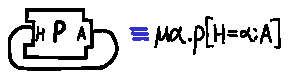
\includegraphics{figures/recursive-unit-identifier.pdf}
\end{figure}

These graphs are equivalent up to unfoldings (i.e., unrolling the
cycles).
As observed in \OldBackpack{}, infinite trees of this form
can be tested for equivalence using Huet's unification algorithm.
However, for an implementation, it is more convenient to compute the canonical form
of a \uid{}, so equality can be checked syntactically.  This can be
computed by Moore machine minimization.  Canonicalization can be achieved
in three steps:

\begin{enumerate}
\item Convert the unit identifier into a Moore machine,
\item Minimize the Moore machine (the procedure is similar to DFA
   minimization, except that states with differing outputs are
   initialized to be in separate equivalence classes initially), and
\item Convert the Moore machine back into a unit identifier.
\end{enumerate}
%
Intuitively, the Moore machine of a unit identifier recognizes paths
(from right to left) through the component graph, outputting the
component identifiers of the component boxes it traverses.

\begin{figure}[H]
\center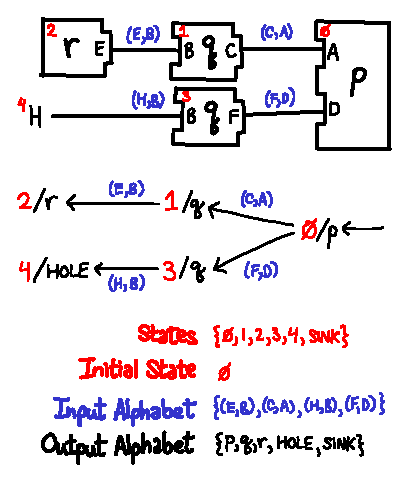
\includegraphics{figures/moore-description.pdf}
\end{figure}

\noindent
Formally, we define the partial Moore machine corresponding to a unit
identifier as follows:

\begin{enumerate}
\item The state set ranges over component boxes and hole modules in the
   graph (in the diagram above, we simply assigned a number to each
   box/hole).
\item The input alphabet is the Cartesian product of output module names
   and input module names.  Intuitively, each member of the alphabet
   corresponds to a wire labeled with the name of the input and output
   ports it is wired to.
\item The output alphabet is the set of component identifiers, as well
   as a distinguished element \verb|HOLE| for hole modules.
\item The inital state is the state corresponding to the component box of
   the unit identifier we want to denote.
\item A transition from $q$ to $q'$ on the input $(m, m')$ exists
   if there is a wire from the input port $m'$ of $q$ to the output
   port $m$ of $q'$ (or a hole module $\hv{m}$, if $q'$ corresponds to a hole
   module).
\item The output of a state is the component identifier of its component
   box, or \verb|HOLE| if it is a hole module.
\end{enumerate}
%
We can complete the partial Moore machine into a total Moore machine by
adding a new sink state \verb|SINK|, which outputs a new output value
\verb|SINK|, and directing all undefined transitions to it (not depicted on
the diagram).

Here are two examples of recursive components expressed as Moore
machines:

\begin{figure}[H]
\center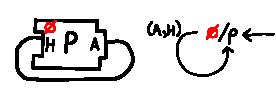
\includegraphics{figures/moore-p.pdf}
\hspace{3em}
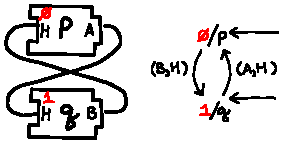
\includegraphics{figures/moore-pq.pdf}
\end{figure}

\noindent
The \uid{} corresponding to a Moore machine is defined by
recursively traversing the Moore machine, creating unit identifiers
whose component identifier is the output at a state, and module
substitution is all of the outgoing transitions to non-sink states. During
this traversal, we maintain a stack of seen states:  when we reach a
state that is already on our stack, we emit a variable bound
for that state on the stack.  This traversal
is guaranteed to terminate as the size of the state set is finite.

\section{Mix-in linking}

Mix-in linking can be straightforwardly adapted to a recursive
setting: the algorithm proceeds as before, but we remove the
occurs check from unification, allowing our unification to
produce infinite trees (as describe above.)  Pictorially,
this simply corresponds to allowing loops when we wire up provisions
to requirements in our component shapes.

\section{Type checking}

The primary complexity of handling recursive linking during type
checking comes down to handling the double vision problem.  To avoid
double vision, typechecking rules must be organized so that the
types/identities of a forward declaration are not used until we finish
computing them.  \OldBackpack{}, MixML and RMC engineer this by
literally separating out this computation as a separate pre-pass.  In
this sketch of recursive linking for \Backpack{}, we'll take a different
approach, taking advantage of the natural staging that occurs in Haskell
typechecking to achieve a similar effect.

\paragraph{Type lookup}
Before we discuss renaming and typechecking for Haskell proper,
it is worth describing how the presence of recursive unit identifiers
affects the type lookup process.  Suppose we're the type of
$\mu\alpha.\, \Mod{\icid{p}{ \subst{A}{\Mod{\alpha}{M}} }}{M}$.
Naively, if we recursively lookup the module types of the modules
in this substitution, so as to construct the required name
substitution, we will suffer from infinite regress.

Fortunately, matters are different if we \emph{lazily} lookup the
original name of a name hole post substitution.  In this situation,
if the original name is well-defined, we will eventually bottom out
with the correct answer.  To detect if an infinite loop has occurred,
we can simply keep track of module identities which we are performing
this lookup for: if a module recurs, we know that we are in an
infinite loop.

Here is a particularly complicated example which demonstrates this
principle:

\begin{lstlisting}
    module A where
        data T = MkT
    signature B where
        data T
    module C(T) where
        import B(T)
    signature D where
        data T
    module E(T) where
        import D(T)
\end{lstlisting}

Suppose this we recursively instantiate this package as per the
following wiring diagram (call this unit identifier $P$):

\begin{figure}[H]
\center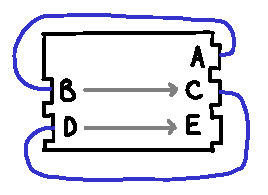
\includegraphics{figures/recursive-uid-example.pdf}
\end{figure}

Suppose we want to look up the original name of the export \verb|T| from
$\Mod{P}{E}$.  We can see in the interface of \verb|D| that,
uninstantiated, \verb|E| exports $\nhv{D.T}$.  By the substitution, this
means we must lookup $\Mod{P}{C}$.  Once again, uninstantiated, \verb|C|
exports $\nhv{B.T}$.  By the substitution, we lookup $\Mod{P}{A}$ and
finally get the true original name of \verb|T|.  If instead \verb|B| was
instantiated with $\Mod{P}{C}$, we would once again lookup $\Mod{P}{C}$
and bail out, as we have discovered an infinite loop.

\paragraph{Renaming}
During renaming, it is necessary to look up the export specifications of
modules we have imported in order to compute the original names of any
reexported entities.  Thus, the key cases in a recursive setting are
handling cases when we are required to look up the export specification
of the module/signature we are currently renaming, or possibly even an
export of a local module/signature which transitively imports the
current module/signature.

In the first case, matters are relatively simple: in a well-typed
module/signature, it is impossible to reexport a forward reference of
this very module/signature, as that would immediately result in a cycle
(reexports cannot rename, and there is always a unique export for any
occurrence name.)

In the second case, there is no way to lookup the export specification
of the local module/signature in question, as it would be a violation of the
no backwards propagation principle to look at the source.  Instead, we
lookup the merged export specification of our dependencies (sans the local
module/signature.)  When the local module/signature is finally typechecked,
we simply need to update the identities in question.

\paragraph{Typechecking}
Handling recursive linking in type checking is easier than with
renaming, because GHC Haskell is already equipped to handle mutually
recursive type definitions within a single module.  In Haskell typechecking,
we first kind-check all type declarations and add them to the environment
(applying any updated definitions to the context), before typechecking
any value declarations.  This means that we never typecheck a value
declaration (the only situation where type-based double vision can
occur) before we have computed the types of all forward declared type
declarations.  One minor complication, as in the renaming case, is that
if we attempt to lookup a type which is not locally defined (either
because it was inherited from a signature, or it comes from a module/signature
which transitively imports us), we should instead defer to the type
from the merge of only the dependencies.

One final remark: one reason why handling double vision in Haskell is so
simple is because we have no mechanism for post-facto \emph{sealing}, unlike
many ML module systems.  Without sealing, we can always compute the types
first, and then handle the values.  With sealing, things are far more complicated:
you must be able to vary which types are transparent and which are opaque when your
have sealed mutually recursive modules.



\bibliographystyle{plain}
\bibliography{references}
\end{document}
